\documentclass[]{usiinfthesis}
\usepackage{lipsum}

% TODO remove this
\usepackage{comment}

%% from the book %%%%%%%%%%%%%%%%%%%%%%%%%%%%%%%%%%%%%%%%%%%%
%\usepackage{amsthm}

\newcommand{\ml}       {\textsc{Matlab}}
\newcommand{\blas}       {\textsc{Blas}}
\newcommand{\lapack}       {\textsc{Lapack}}
\newcommand{\nl}{\scriptstyle{0}}
\newcommand{\mmd}       {\textsc{Mmd}}
\newcommand{\amd}       {\textsc{Amd}}
\newcommand{\cC}{\mathcal{C}}
\newcommand{\cI}{\mathcal{I}}
\newcommand{\cK}{\mathcal{K}}
\newcommand{\cM}{\mathcal{M}}
\newcommand{\colamd}       {\textsc{Colamd}}
\newcommand{\rcm}       {\textsc{Rcm}}
\newcommand{\metis}     {\textsc{Metis}}
\newcommand{\parmetis}     {\textsc{ParMetis}}
\newcommand{\mtmetis}     {\textsc{MT-Metis}}
\newcommand{\scotch}     {\textsc{Scotch}}
\newcommand{\mat}[1]{\left(\begin{array}{#1}}
\newcommand{\rix}{\end{array}\right)}
\newcommand{\R}{\mathbb{R}}
\newcommand{\circn}[1]{{\large$\bigcirc\mkern-18.7mu$}$#1\;\mkern\medmuskip$}
% bold math and symbol, e.g. for vector
%\newcommand{\bm}[1]{\textbf{#1}}
%\newcommand{\bs}[1]{\boldsymbol{#1}}
%
%\newcommand{\mctwo}[1]{\multicolumn{2}{c}{#1}}
%\newcommand{\mltwo}[1]{\multicolumn{2}{l|}{#1}}
%
%\newcommand{\nxlnz}{xl}
%\newcommand{\nlnz}{l}
%\newcommand{\nindx}{id}
%\newcommand{\nxindx}{xid}
%\newcommand{\nr}{r}
%\newcommand{\ntemp}{t}
%
%\newcommand{\vxlnz}{\texttt{\nxlnz{}}}
%\newcommand{\vlnz}{\texttt{\nlnz}}
%\newcommand{\vxindx}{\texttt{\nxindx}}
%\newcommand{\vindx}{\texttt{\nindx}}
%\newcommand{\vr}{\texttt{\nr}}
%\newcommand{\vtemp}{\texttt{\ntemp}}
%
%\newcommand{\cyw}{\text{cy}}
%\newcommand{\mv}[1]{\textbf{#1}}
%
%\newcommand{\bi}{\begin{itemize}}
%\newcommand{\ei}{\end{itemize}}
%
%\newcommand{\be}{\begin{equation}}
%\newcommand{\ee}{\end{equation}}
%%%%%%%%%%%%%%%%%%%%%%%%%%%%%%%%%%%%%%%%%%%%%%

%% I hope this works %%%%%%%%%%%%%%%%%%%%%%%%%
%\usepackage{amsthm}
%\theoremstyle{definition}
%\newenvironment{definition}[1][section]{Definition: #1}
\newtheorem{theorem}{Theorem}[section]
\newtheorem{definition}{Definition}[section]
\newtheorem{remark}{Remark}[section]
%\theoremstyle{definition}

\def\formtmp#1#2{{\vskip12pt\noindent\fboxsep=0pt\colorbox{#1}{\vbox{\vskip3pt\hbox to \textwidth{\hskip3pt\vbox{\raggedright\noindent\textbf{#2\vphantom{Qy}}}\hfill}\vspace*{3pt}}}\par\vskip2pt%
\noindent\kern0pt}}

\RequirePackage[x11names]{xcolor}
\definecolor{example}{gray}{0.85}
%\newenvironment{example}[1]{\ignorespaces\def\stmtopen##1{##1}%
%\formtmp{example}{#1}}{\par\noindent\textcolor{example}{\rule{\columnwidth}{1pt}}\vskip2pt\par\addvspace{\baselineskip}}%
\newenvironment{example}[1]{\ignorespaces\def\stmtopen##1{##1}%
\formtmp{example}{#1}}{\par\noindent\textcolor{example}{\rule{\columnwidth}{1pt}}\vskip2pt\par\addvspace{\baselineskip}}%

\definecolor{programcode}{gray}{0.65}
\newenvironment{programcode}[1]{\ignorespaces\def\stmtopen##1{##1}%
\formtmp{programcode}{#1}}{\noindent\textcolor{programcode}{\rule{\columnwidth}{1pt}}\vskip2pt\par\addvspace{\baselineskip}}%

\usepackage{multirow}

\usepackage{algorithm}
\usepackage{algorithmicx}
\usepackage{algpseudocode}


%4-class OrRd Tokyo SIAM PP18
\definecolor{mycolor0}{HTML}{2B83BA}
\definecolor{mycolor1}{HTML}{D7301F}
\definecolor{mycolor2}{HTML}{FC8D59}
\definecolor{mycolor3}{HTML}{abdda4}
\definecolor{mycolor4}{HTML}{e9a3c9}
\definecolor{mycolor5}{HTML}{FEF0D9}


\usepackage{wrapfig}


\usepackage{graphicx}
\usepackage[caption=false]{subfig}
\usepackage{sidecap}

%\newcommand{\panelsize}{s}

\usepackage{algorithm}
\usepackage{algpseudocode} % part of the algorithmicx package
  % Indent each nesting level only by 1em 
  \algrenewcommand\algorithmicindent{1em}%
  
  
%\usepackage[
%  debug,
%  a4paper, 
%  colorlinks=true, 
%  linkcolor=blue, 
%  citecolor=blue, 
%  urlcolor=blue, 
%  bookmarksopen=true, 
%  bookmarksnumbered=true
%]{hyperref}

\newcommand{\xximg}[3]{%
  \subfloat[#2]{%
    \includegraphics[height=3cm,clip=true]{{{images/perf/p-80/p-#1-#3}}}%
  } \,%
}

\newcommand{\perfimages}[1]{
  \xximg{#1}{lapl1}{n-40-b-4}
  \xximg{#1}{lapl2}{n-70-b-1}
  \xximg{#1}{omen1}{omen-rgf-tc2.5-lc160}
  \xximg{#1}{omen2}{omen-rgf-tc3.5}
  \xximg{#1}{omen3}{omen-rgf-tc4.5}
}

\newcommand{\ximg}[3]{%
  \subfloat[#1]{%
    \includegraphics[height=3cm,clip=true]{{{images/perf/p-80/p-#3-#2}}}%
  } \,%
}

\newcommand{\pimages}[2]{
  \ximg{#1}{#2}{emmy}%
  \ximg{#1}{#2}{hasep1}%
  \ximg{#1}{#2}{woody-hsw}%
  \ximg{#1}{#2}{meggie}%
  \ximg{#1}{#2}{knightmare1}%
  \ximg{#1}{#2}{summitridge1}%
  \ximg{#1}{#2}{sxace}

}

\newcommand{\mv}[1]{\textbf{#1}}

\newcommand{\bi}{\begin{itemize}}
\newcommand{\ei}{\end{itemize}}

\newcommand{\be}{\begin{equation}}
\newcommand{\ee}{\end{equation}}

\newcommand{\todo}[1]{ {\quad\color{red}!!!#1!!!\quad} }

%\newcommand{\doiurl}[2][]{#1\href{http://dx.doi.org/#2}{\nolinkurl{#2}}}
%%\newcommand{\bibdoiurl}[1]{\doiurl[doi:]{#1}}
%\newcommand{\bibdoiurl}[1]{DOI:#1}

\newcommand{\arxurl}[2][]{#1\href{http://arxiv.org/abs/#2}{\nolinkurl{#2}}}
% \newcommand{\bibarxurl}[1]{\arxurl[arXiv:]{#1}}
\newcommand{\bibarxurl}[1]{arXiv:#1}

% bold math and symbol, e.g. for vector
\newcommand{\bm}[1]{\textbf{#1}}
\newcommand{\bs}[1]{\boldsymbol{#1}}

\newcommand{\mymat}[1]{\textit{#1}}

\newcommand{\mctwo}[1]{\multicolumn{2}{c}{#1}}
%\newcommand{\mltwo}[1]{\multicolumn{2}{l|}{#1}}
\newcommand{\mltwo}[1]{\multicolumn{2}{l}{#1}}
\newcommand{\mlfour}[1]{\multicolumn{4}{l}{\scriptsize #1}}
\newcommand{\mcct}[1]{\multicolumn{3}{c}{#1}}

\usepackage{ulem} % sout uwave


\newcommand{\nxlnz}{xl}
\newcommand{\nlnz}{l}
\newcommand{\nindx}{id}
\newcommand{\nxindx}{xid}
\newcommand{\nr}{r}
\newcommand{\ntemp}{t}

\newcommand{\vxlnz}{\texttt{\nxlnz{}}}
\newcommand{\vlnz}{\texttt{\nlnz}}
\newcommand{\vxindx}{\texttt{\nxindx}}
\newcommand{\vindx}{\texttt{\nindx}}
\newcommand{\vr}{\texttt{\nr}}
\newcommand{\vtemp}{\texttt{\ntemp}}

\newcommand{\cyw}{\text{cy}}
\newcommand{\Bw}{\text{B}}

% Symbol used to denote the panel size.
\newcommand{\panelsize}{s}

\setlength{\tabcolsep}{1pt}
\setcounter{tocdepth}{1}


\usepackage{algorithmicx}

\usepackage{adjustbox}


\usepackage{tikz}
\usepackage{pgfplots}
\pgfplotsset{compat=1.8}
%\usetikzlibrary{automata}
\usetikzlibrary{patterns}
\usepackage{float}
\usepackage{listings}

% fix missing "*" in listings
\renewcommand{\textasteriskcentered}{\ensuremath{*}}

\usepackage{array}

\usepackage{color}
\newcommand{\todol}[1]{\textbf{\textcolor{red}{[[#1]]}}}
\newcommand{\todop}[1]{\noindent\textbf{\textcolor{red}{[[#1]]}}\\}

\newcommand{\doiurl}[2][]{#1\href{http://dx.doi.org/#2}{\nolinkurl{#2}}}
\newcommand{\bibdoiurl}[1]{\doiurl[doi:]{#1}}

%\usepackage[draft]{fixme}

%change 'sl' to 'bf' for bold, or 'normalfont' for no special
%formatting
\captionsetup{labelfont={sl,sf}}

\lstdefinelanguage{algebra}
{morekeywords={import,sort,constructors,observers,transformers,axioms,if,
else,end},
sensitive=false,
morecomment=[l]{//s},
}


\title{Node-Level Performance Modeling \\of Sparse Factorization Solver} %compulsory
%\subtitle{Subtitle: Reinventing the World} %optional 
\advisor{Prof. Olaf Schenk} %compulsory
\committee{%
  %\committeeMember{Alonzo Church}{University of California, Los Angeles, USA}
  %\committeeMember{Alan M. Turing}{Princeton University, USA}
  \committeeMember{Prof. Illia Horenko}{Universit\`a della Svizzera italiana, Switzerland}
  \committeeMember{Prof. Igor Pivkin}{Universit\`a della Svizzera italiana, Switzerland}
  \committeeMember{Prof. Harald K\"ostler}{Friedrich-Alexander University Erlangen-Nurnberg, Germany}
  \committeeMember{Prof. Tom\'a\v{s} Kozubek}{Technical University of Ostrava, Czech Republic}
  %there can as many members as you like
} %the committee is compulsory
\author{Radim Janal\'ik} %compulsory
%\coadvisor{Co-Advisor} %optional
\Day{\todol{TBD}} %compulsory
\Month{August} %compulsory
\Year{2021} %compulsory, put only the year
\place{Lugano} %compulsory
%\programDirector{Prof. Olaf Schenk \emph{pro tempore}} %compulsory
\programDirector{Prof. Walter Binder\\ & \textbf{Prof. Silvia Santini}} %compulsory

%\dedication{To my beloved} %optional
%\openepigraph{Someone said \dots}{Someone} %optional

\makeindex %optional, also comment out \theindex at the end

\begin{document}

\maketitle %generates the titlepage, this is FIXED

\frontmatter %generates the frontmatter, this is FIXED

\begin{abstract}
Solving large sparse linear systems is at the heart of many application problems arising from scientific and engineering problems. These systems are often solved by direct factorization solvers, especially when the system needs to be solved for multiple right-hand sides or when a high numerical precision is required.
Direct solvers are based on matrix factorization, which is then followed by forward and backward substitution to obtain a precise solution. The factorization is the most computationally intensive step, but it has to be computed only once for a given matrix. Then the system is solved with forward and backward substitution for every right-hand side.
Performance modeling of algorithms involved in solving these linear systems reveals the computational bottlenecks, which can guide node-level performance optimizations and shows the best performance that can be achieved.
The Berkeley roofline model is widely used to predict the upper bound of a code based on processor peak performance and memory bandwidth. Modification of the Roofline model allows us to model performance of forward and backward substitution codes, which are a combination of sequential and parallel execution. The model predictions are compared with various measurements for a representative set of sparse matrices on different x86\_64 processors.
\end{abstract}

\begin{acknowledgements}
\todop{\lipsum} 
\end{acknowledgements}

\tableofcontents 
%\listoffigures %optional
%\listoftables %optional

\mainmatter

\chapter{Overview of State-of-The-Art Sparse Direct Solvers}

%\begin{chapter_preamble}
This chapter presents an overview of combinatorial algorithms in sparse elimination methods.
Beside well-established techniques that have been developed in the last twenty years a modern
viewpoint of sparse $LU$ and $LDL^T$ decomposition is presented that illustrates how the
evolution of techniques in the last decade improved the performance of sparse direct solvers by
three to four orders of magnitude. Some parts of this chapter have been published as an invited
overview paper on parallel sparse direct methods in \cite{Bollhofer2020}.
%\end{chapter_preamble}

\section{Introduction}
\label{sec:intro}
Solving large sparse linear systems is at the heart of many application
problems arising from computational science and engineering applications.
Advances in combinatorial
methods in combination with modern computer architectures have massively
influenced the design of state-of-the-art direct solvers
that are feasible for solving  larger systems efficiently
in a computational environment with rapidly increasing memory resources
and cores. Among these advances are 
novel combinatorial algorithms for improving diagonal dominance which
pave the way to a static pivoting approach, thus improving the 
efficiency of the factorization
phase dramatically. Besides, partitioning and reordering the system
such that a high level of concurrency is achieved, the objective is to 
simultaneously achieve the reduction of fill-in and the parallel concurrency.
While these achievements already significantly improve the factorization
phase, modern computer architectures require one to compute as many operations
as possible in the cache of the CPU. This in turn can be achieved when
dense subblocks that show up during the factorization can be grouped
together into dense submatrices which are handled
by multithreaded and cache-optimized 
dense matrix kernels using level-3 BLAS and LAPACK
(\cite{AndBBDDDGHMOS95}).

This chapter will review some of the basic technologies together
with the latest developments for sparse direct solution methods that have led to
state-of-the-art $LU$ decomposition methods.
The paper is organized as follows. In Section \ref{sec:mwm}
we will start with maximum weighted matchings which is one of the key
tools in combinatorial optimization to dramatically improve the diagonal dominance
of the underlying system.
Next, Section \ref{sec:reordering} will review multilevel nested dissection
as a combinatorial method to reorder a system symmetrically
such that fill-in and parallelization are improved simultaneously, once
pivoting can be more or less ignored.
After that, we will review established graph-theoretical approaches
in Section \ref{sec:lu}, in particular the elimination tree, from which
most of the properties of the $LU$ factorization can be concluded. Among
these properties is the prediction of dense submatrices in the
factorization. In this way several subsequent
columns of the factors $L$ and $U^T$ are collected in a single dense block. 
This is the basis for the use of dense matrix kernels using optimized
level-3 BLAS as well to exploit fast computation using the cache hierarchy which 
is discussed in Section~\ref{sec:parallel}.
%Finally, we show in Section~\ref{sec:appl} how the ongoing developments in parallel sparse direct solution methods have advanced integrated circuit simulations.
We assume that the reader
 is familiar with some elementary knowledge from
graph theory, see; e.g., \cite{DufER86,GeoL81} and some simple
computational algorithms based on graphs \cite{AhoHU83}.

\section{Maximum weight matching to enable static data structures}
\label{sec:mwm}
In modern sparse elimination methods the key to success 
is ability to work with efficient data structures and their underlying
numerical templates. If we can increase the size of the diagonal entries
as much as possible in advance, pivoting during Gaussian elimination can often 
be bypassed and we may work with static data structures and
the numerical method will be significantly accelerated. 
A popular method to achieve this goal is the
maximum weight matching method~(\cite{DufK99S,olschowka:1996})
which permutes (e.g.) the rows of a given
nonsingular matrix $A\in\R^{n,n}$ by a permutation matrix $\Pi\in\R^{n,n}$ 
such that $\Pi^TA$
has a non-zero diagonal. Moreover, it maximizes
the product of the absolute diagonal values  and yields diagonal
scaling matrices $D_r, D_c\in\R^{n,n}$ such that $\tilde A=\Pi^TD_rAD_c$ satisfies
$|\tilde a_{ij}|\leqslant 1$ and $|\tilde a_{ii}|=1$ for all $i,j=1,\dots,n$.
The original idea on which these nonsymmetric permutations and scalings are
based is to find a maximum weighted matching of a
bipartite graphs. Finding a maximum weighted matching is a well
known assignment problem in operation research and combinatorial
analysis.
\begin{definition}\label{def:bipartite}
A graph $G=(V,E)$ with vertices $V$ and edges $E\subset V^2$ 
is called bipartite
if $V$ can be partitioned into two sets  $V_r$ and  $V_c$, such that no edge
$e=(v_1,v_2) \in E$ has both ends $v_1,v_2$ in $V_r$ or both ends $v_1,v_2$ 
in $V_c$. In this case we denote $G$ by $G_b=(V_r,V_c,E)$.
\end{definition}
%\begin{definition}
%For $A\in\R^{n,n}$ its associated graph is given $G(A)=(V,E)$,
%where $V=\{1,\dots,n\}$ and $E=\{(i,j)|\; a_{ij}\not=0\}$.
%\end{definition}
\begin{definition}\label{def:bipartite-graph}
Given a matrix $A$, then we can associate with it a canonical
bipartite graph $G_b(A)=(V_r,V_c,E)$ by assigning the 
labels of $V_r=\{r_1,\dots,r_n\}$ 
with the row indices of $A$ and 
$V_c=\{c_1,\dots,c_n\}$ being labeled by the column indices.
In this case $E$ is defined via $E=\{(r_i,c_j)|\; a_{ij}\not=0\}$.
\end{definition}
For the bipartite graph $G_b(A)$ we see immediately that 
If $a_{ij}\not=0$, 
then we have that $r_i \in V_r$ from the row set
is connected by an edge $(r_i,c_j) \in E$ to the column $c_j \in V_c$,
but neither rows are connected with each other nor do the columns have
inter connections.
\begin{definition}\label{def:matching}
A matching $\cM$
of a given graph $G= (V,E)$ is a subset of edges
$e\in E$ such that no two of which share the same vertex. 
\end{definition}
If $\cM$ is a
matching of a bipartite graph $G_b(A)$, then each edge $e=(r_i,c_j) \in \cM$ 
corresponds to a row $i$ and a column $j$ and there exists no other edge 
$\hat e=(r_k,c_l) \in \cM$ 
that has the same vertices, neither $r_k=r_i$ nor $c_l=c_j$. 
\begin{definition}\label{def:maxmatching}
A matching $\cM$ of $G=(V,E)$ is called
maximal, if no other edge from $E$ can be added to $\cM$.
\end{definition}
If, for an $n \times n$ matrix $A$ a matching $\cM$ of $G_b(A)$ with
maximum cardinality $n$ is found, then by definition the edges 
must be $(i_1,1),\dots,(i_n,n)$ with $i_1,\dots,i_n$ being the 
numbers $1,\dots,n$ in a suitable order and therefore we obtain
$a_{i_1,1}\not=0$, \dots
$a_{i_n,n}\not=0$. In this case 
we have established that the
matrix $A$ is at least structurally nonsingular and we can use a 
row permutation matrix $\Pi^T$ associated with row ordering $i_1,\dots,i_n$ 
to place a nonzero entry on each diagonal location of $\Pi^TA$.
\begin{definition}\label{def:perfect-matching}
A perfect matching is a maximal matching with cardinality $n$.
\end{definition}
It can be shown that for a structurally nonsingular matrix $A$ there always
exists a perfect matching $\cM$.
%\begin{theorem}\label{hopcraft}
%When $A\in\R^{n,n}$ is structurally nonsingular, then 
%there always exists  a perfect
%matching for $G_b(A) = (V_r, V_c, E)$. The perfect matching $\cM$ defines
%an $n \times n$ permutation matrix with
%\[
%\Pi^T = (p_{ij}) =  \left\{ 
%\begin{array}{cc} 
%p_{ij} = 1 & e_{ij} \in M \\
%p_{ij} = 0 & e_{ij} \not \in M  
%                          \end{array} \right.
%\]
%\end{theorem}
\begin{example}{Perfect Matching}\label{exm:perfect_matching}
In Figure \ref{fig:unsym_perm}, the set of edges $\cM= \{(1,2), (2,4),
(3,5), (4,1), (5,3), (6,6) \}$ represents a perfect maximum matching
of the bipartite graph $G_b(A)$.
\end{example}
\begin{figure}
% \sidecaption
\begin{minipage}{.33\textwidth}
 \begin{center}
 Original Matrix $A$
    $\left(
%
        \begin{array}{cccccc}
         % 1 & 3 & \nl &  2 & \nl & \nl \\
         1 & 3 & \nl & \nl & \nl & \nl \\
          3  & \nl & \nl & 4 & \nl & 1 \\
        \nl & \nl & \nl & \nl &  3  & \nl \\
        % 2 &  4  & \nl & \nl & 1 & \nl \\
        2 &  \nl  & \nl & \nl & 1 & \nl \\
        \nl & \nl &  3  & 1 & \nl & \nl \\
        \nl & 1 & \nl & \nl & \nl &  2
        \end{array}
    \right) $ 
 \end{center}
\end{minipage}
\begin{minipage}{.32\textwidth}
 \begin{center}
$G_b(A): \;$ 
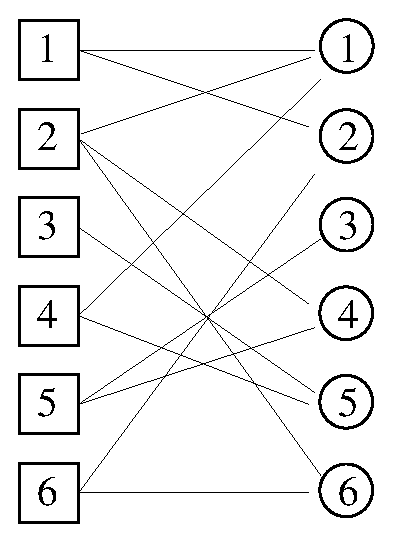
\includegraphics[width=0.43\textwidth]{figures/matching1} 
%
%\medskip
%
\hspace{0.5cm}$\cM: \;$ 
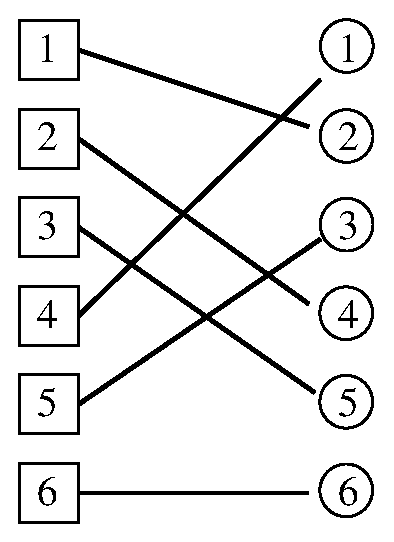
\includegraphics[width=0.43\textwidth]{figures/matching2} 
 \end{center}
\end{minipage}
\begin{minipage}{.32\textwidth}
  \begin{center}
Reordered Matrix $\Pi^TA$

    $\left(
        \begin{array}{cccccc}
        % 2 &  4  & \nl & \nl & 1 & \nl \\
        2 &  \nl  & \nl & \nl & 1 & \nl \\
        % 1 & 3 & \nl &  2 & \nl & \nl \\
         1 & 3 & \nl &  \nl & \nl & \nl \\
        \nl & \nl &  3  & 1 & \nl & \nl \\
         3  & \nl & \nl & 4 & \nl & 1 \\
        \nl & \nl & \nl & \nl &  3  & \nl \\
        \nl & 1 & \nl & \nl & \nl &  2
        \end{array}
    \right) $ 
% \medskip
 \end{center}  
\end{minipage}
    \caption{Perfect matching. Left side: original
      matrix $A$. Middle: bipartite representation $G_b(A) = (V_r, V_c, E)$
      of the matrix $A$ and perfect matching $\cM$. Right side: permuted matrix
      $\Pi^TA$.}
    \label{fig:unsym_perm}
\end{figure}

The most efficient combinatorial methods for finding maximum matchings
in bipartite graphs make use of an augmenting path. We will
introduce some graph terminology for the
 construction of perfect
matchings. 
\begin{definition}\label{def:path}
If an edge $e=(u,v)$ in a graph $G=(V,E)$
joins a vertices $u,v\in V$, then we denote it as $uv$. 
A path then consists of edges $u_1u_2,u_2u_3,u_3u_4 \ldots,u_{k-1}u_k$, where 
each $(u_i,u_{i+1})\in E$, $i=1,\dots,k-1$.
\end{definition}
If $G_b=(V_r,V_c,E)$ is a bipartite graph, then by definition of a path, 
any path is alternating between the vertices of $V_r$ and $V_c$, e.g.,
paths in $G_b$ could be such as $r_1c_2,c_2r_3,r_3c_4,\dots$.
\begin{definition}\label{def:various-paths}
Given a graph $G=(V,E)$, a 
vertex is called free if it is not
incident to any other edge in a matching $\cM$ of $G$. 
An alternating path relative to a matching $\cM$ is a path
$P = u_1u_2,u_2u_3, \ldots,u_{s-1}u_s$ where its edges are alternating 
between $E \setminus \cM$ and $\cM$. An
augmenting path relative to a matching $\cM$ is an alternating
path of odd length and both of it vertex endpoints are free. 
\end{definition}
\begin{example}{Augmenting Path}\label{exm:augmenting_path}
Consider Figure \ref{fig:unsym_perm}.
To better distinguish between row and column vertices we use
$\fbox{$1$},\fbox{$2$},\dots,\fbox{$6$}$ for the rows and \circn{1},\circn{2},\dots,\circn{6} for the
columns.
A non-perfect but maximal matching is given by
$M= \{(\fbox{$4$},$\circn{5}$), (\fbox{$1$},$\circn{1}$), (\fbox{$6$},$\circn{2}$),\\ (\fbox{$2$},$\circn{6}$), (\fbox{$5$},$\circn{4}$) \}$.
We can easily see that an augmenting path 
alternating between rows and columns is given by \fbox{$3$}\circn{5} , \circn{5}\fbox{$4$} , \fbox{$4$}\circn{1} , \circn{1}\fbox{$1$} , \fbox{$1$}\circn{2}~, \circn{2}\fbox{$6$} , \fbox{$6$}\circn{6} , \circn{6}\fbox{$2$} , \fbox{$2$}\circn{4} , \circn{4}\fbox{$5$} , \fbox{$5$}\circn{3}. Both endpoints \fbox{$3$} and \circn{3}
of this augmenting path are free.
\end{example}

In a bipartite
graph $G_b= (V_r, V_c, E)$ one vertex endpoint of any
augmenting path must be in $V_r$ whereas the other one must be in $V_c$. 
The symmetric
difference, $A \oplus B$ of two edge sets $A$, $B$ is defined to be $(A
\setminus B) \cup (B \setminus A)$.

Using these definitions and notations,
the following theorem (\cite{Berge}) gives a
constructive algorithm for finding perfect matchings in bipartite
graphs.

\begin{theorem}\label{theo:Berge}
If $\cM$ is non-maximum matching of a bipartite graph $G_b= (V_r, V_c,E)$, 
then there exists an augmenting path $P$ relative to $\cM$ such that
 $P=\tilde{\cM} \oplus \cM$ and $\tilde{\cM}$
is a matching with cardinality $|\cM|+1$.
\end{theorem}
According to this theorem, a combinatorial method of finding perfect
matching in a bipartite graph is to seek augmenting paths. 

The
perfect matching as discussed so far only takes the nonzero structure
of the matrix into account. 
For their use as static pivoting methods prior to the $LU$ decomposition
one requires in addition to
maximize the absolute value of the product of the diagonal entries. 
This is referred to as
maximum weighted matching. In this case a permutation
$\pi$ has to be found, which maximizes
\begin{equation}
  \prod_{i=1}^n |a_{\pi(i)i}|. \label{eq:1}
\end{equation}
The maximization of this product is transferred into a minimization of a sum as follows. We define a matrix $C = (c_{ij})$ via
\[
  c_{ij} = 
  \begin{cases}
    \log a_i - \log |a_{ij}| & a_{ij} \neq 0 \\
    \infty                     & \text{otherwise},
  \end{cases}
\]
where $a_i = \max_j |a_{ij}|$  is the maximum element in row $i$ of
matrix $A$. A permutation $\pi$ which minimizes the sum 
\[
  \label{eq:4}
  \sum_{i=1}^n c_{\pi(i)i} 
\]
also maximizes the product~(\ref{eq:1}). The minimization problem is
known as linear-sum assignment problem or bipartite weighted matching
problem in combinatorial optimization.  The problem is solved by a
sparse variant of the Hungarian method. The complexity is
 $\mathcal{O}(n \tau \log n )$ for
sparse matrices with $\tau$ entries. For matrices, whose associated
graph fulfill special requirements, this bound can be reduced further
to $\mathcal{O}(n^\alpha (\tau + n \log n))$ with $\alpha < 1$.  All graphs
arising from finite-difference or finite element discretizations meet
the conditions~(\cite{gupta:99}). As before, we finally get a perfect
matching which in turn defines a nonsymmetric permutation.

When solving the assignment problem, two dual vectors $u = (u_i)$ and
$v = (v_i)$ are computed which satisfy
\begin{align}
  u_i + v_j & = c_{ij} \qquad  (i,j) \in \cM, \label{eq:11} \\
  u_i + v_j & \leq c_{ij} \qquad \text{otherwise}. \label{eq:12}
\end{align}
Using the exponential function these vectors can be used to scale the 
initial matrix. To do so define
two diagonal matrices $D_r$ and $D_c$ through
\begin{align}
  D_r & = \text{diag}(d_1^r,d_2^r,\dots,d_n^r), \qquad d_i^r = \exp(u_i),\\ 
  D_c & = \text{diag}(d_1^c,d_2^c,\dots,d_n^c), \qquad d_j^c = \exp(v_j)/a_j.
\end{align}
Using equations (\ref{eq:11}) and (\ref{eq:12}) and the definition of $C$, 
it immediately follows that $\tilde A = \Pi^T D_r A D_c$ satisfies
\begin{align}
  |\tilde a_{ii}| & = 1, \label{eq:13}\\
  |\tilde a_{ij}| & \le 1. \label{eq:14}
\end{align}
The permuted and scaled system $\tilde A$ has been observed to
have significantly better numerical properties when being used
for direct methods or for preconditioned iterative methods, cf. e.g. 
\cite{benzi:2000:phi,DufK99S}. \cite{olschowka:1996} introduced these scalings and
permutation for reducing pivoting in Gaussian elimination of full
matrices. The first implementation for sparse matrix problems was
introduced by \cite{DufK99S}. For symmetric
matrices $|A|$, these nonsymmetric matchings can be converted
to a symmetric permutation $P$ and a symmetric scaling $D_s=(D_rD_c)^{1/2}$
such that $P^TD_sAD_sP$ consists mostly of diagonal blocks of size $1\times 1$
and $2\times 2$ satisfying a similar condition as (\ref{eq:13}) and (\ref{eq:14}),
where in practice it rarely happens that  $1\times 1$ blocks are identical 
to $0$~(\cite{dupr:04a}).
Recently, successful parallel approaches to compute maximum weighted matchings have
been proposed~(\cite{LanPM11,LanAM14}).

\begin{example}{Maximum Weight Matching}\label{exm:west0479-match}
To conclude this section we demonstrate the effectiveness of maximum weight matchings using a simple sample matrix ``west0479'' from the SuiteSparse Matrix Collection.
The matrix can also directly be loaded in \ml{} using \texttt{load west0479}.
In Figure \ref{fig:mwm} we display the matrix before and after applying maximum
weighted matchings. To illustrate the improved diagonal dominance we further
compute $r_i=|a_{ii}|/\sum_{j=1}^n|a_{ij}|$ for each row of $A$ and $\tilde A=\Pi^TD_rAD_s$, $i=1,\dots,n$. $r_i$ can be read as relative diagonal dominance of row $i$ 
and yields a number between $0$ and $1$. Moreover, whenever $r_i>\frac12$, the row
is strictly diagonal dominant, i.e., $|a_{ii}|>\sum_{j:j\not=i}|a_{ij}|$.
In Figure \ref{fig:mwm} we display for both matrices $r_i$ by sorting its values
in increasing order and taking $\frac12$ as reference line. We can see the
dramatic impact of maximum weighted matchings in improving the diagonal dominance
of the given matrix and thus paving the way to a static pivoting approach
in incomplete or complete $LU$ decomposition methods.
\end{example}
\begin{figure}
% \sidecaption
\begin{minipage}{.45\textwidth}
 \begin{center}
% Original Matrix $A$
%
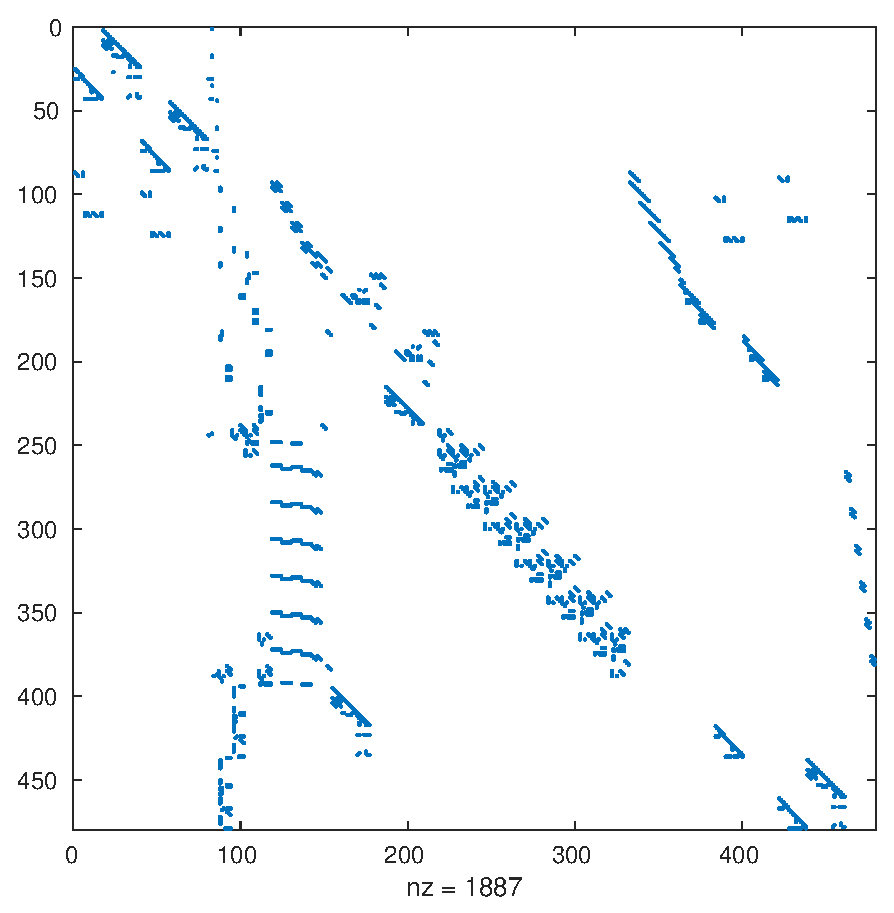
\includegraphics[width=0.8\textwidth]{figures/west0479} 
 \end{center}
\end{minipage}
~
\begin{minipage}{.45\textwidth}
  \begin{center}
%Reordered and Rescaled Matrix 
%
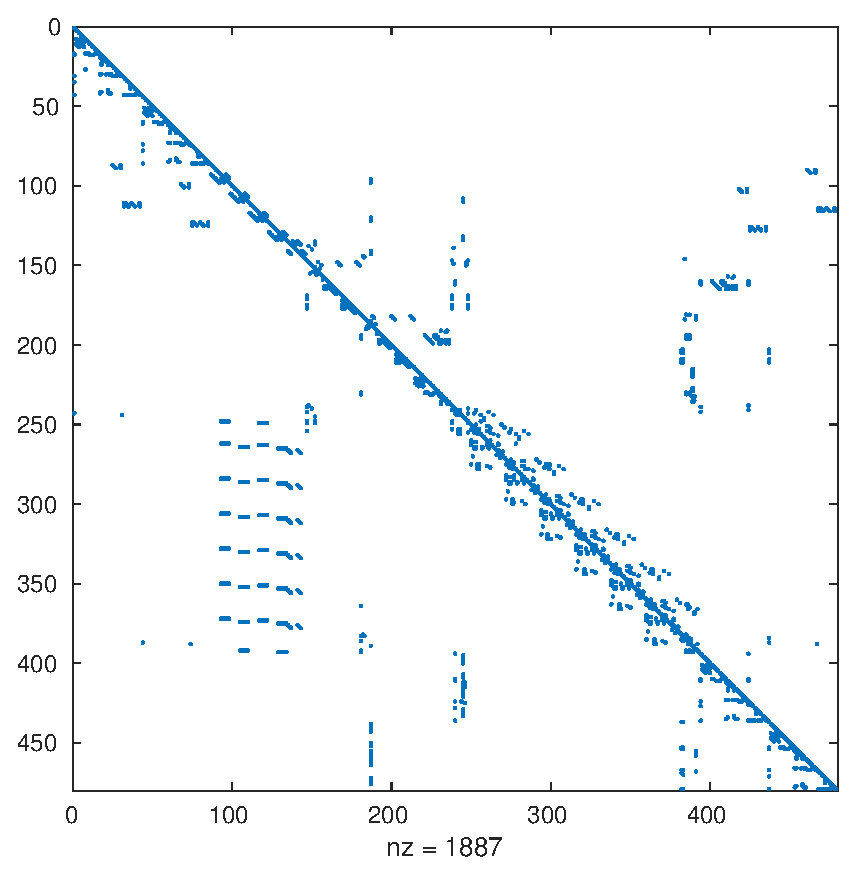
\includegraphics[width=0.8\textwidth]{figures/west0479-match} 
 \end{center}  
\end{minipage}
    \caption{Maximum weight matching. Left side: original
      matrix $A$. Right side: permuted and rescaled matrix
      $\tilde A=\Pi^TD_rAD_c$.}
    \label{fig:mwm}
\end{figure}
\begin{figure}
% \sidecaption
\begin{minipage}{.48\textwidth}
 \begin{center}
% Original Matrix $A$
%
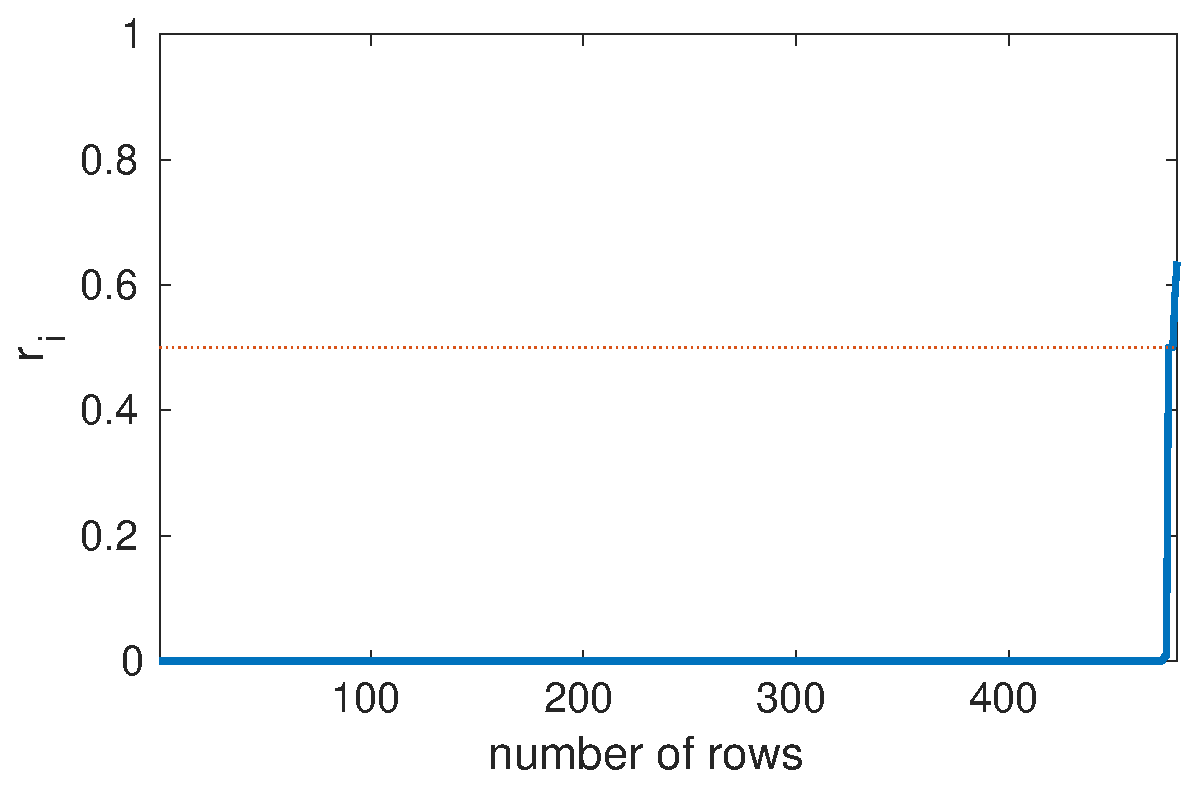
\includegraphics[width=0.95\textwidth,height=0.5\textwidth]{figures/west0479-dd} 
 \end{center}
\end{minipage}
~
\begin{minipage}{.48\textwidth}
  \begin{center}
%Reordered and Rescaled Matrix 
%
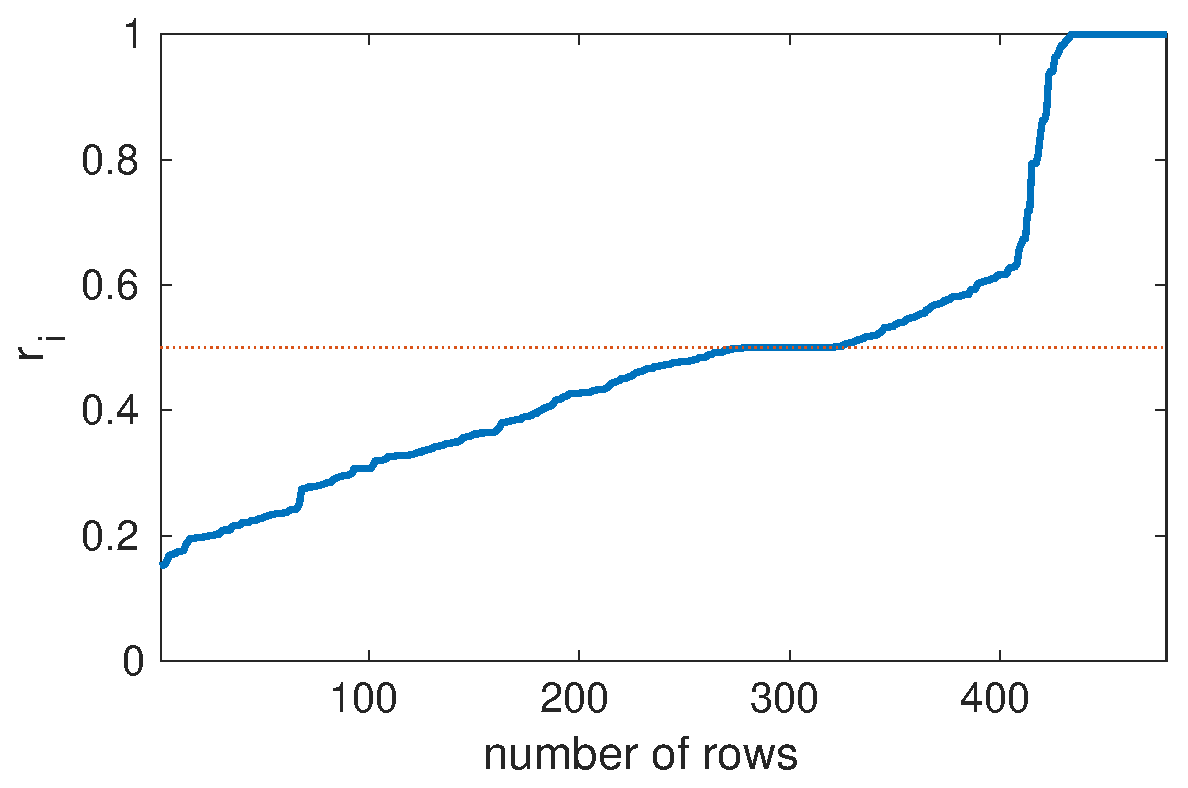
\includegraphics[width=0.95\textwidth,height=0.5\textwidth]{figures/west0479-match-dd} 
 \end{center}  
\end{minipage}
    \caption{Diagonal dominance. Left side: $r_i$ for $A$. Right side: $r_i$  $\tilde A=\Pi^TD_rAD_c$.}
    \label{fig:mwm-dd}
\end{figure}

\section[Symbolic reordering techniques based on nested dissection]{Symbolic reordering techniques based on Multilevel nested dissection} 
\label{sec:reordering}
When dealing with large sparse matrices a crucial factor that determines
the computation time is the amount of fill that is produced during the
factorization of the underlying matrix. To reduce the complexity there
exist many mainly symmetric reordering techniques that attempt to reduce
the fill-in heuristically. Here we will demonstrate only one of these
methods, the so-called nested dissection method. The main reason for selecting
this method is that it can be easily used for parallel computations.

%\subsection{Multilevel nested dissection}
\label{subsec:mnd}
Recursive multilevel nested dissection methods for direct
decomposition methods were first introduced in the context of
multiprocessing. If parallel direct methods are used to solve a sparse
system of equations, then a graph partitioning algorithm can be used
to compute a fill reducing ordering that leads to a high degree of
concurrency in the factorization phase. 
\begin{definition}\label{def:matrix-graph}
For a matrix $A\in\R^{n,n}$ we
 define the associated (directed) graph $G_d(A)=(V,E)$, where 
$V=\{1,\dots,n\}$ and the set of edges 
$E=\left\{(i,j)|\, a_{ij}\not=0\right\}$.
The (undirected) graph is given by  $G_d(|A|+|A|^T)$ and is denoted
simply by $G(A)$.
\end{definition}
In graph terminology for a sparse matrix $A$ we simply have a directed
edge $(i,j)$ for any nonzero entry $a_{ij}$ in $G_d(A)$ whereas the 
orientation of the edge is ignored in $G(A)$.

The research on graph-partitioning
methods in the mid-nineties has resulted in high-quality software
packages, e.g. \metis {} (\cite{karypis:98}).
These methods often compute orderings that on the one hand lead to small fill-in 
for (incomplete) factorization methods while on the other hand they
provide a high level of concurrency.
We will briefly review the main idea of multilevel nested dissection in
terms of graph-partitioning.
\begin{definition}\label{def:partitioning-and-separator}
Let $A\in\R^{n,n}$
and consider its graph $G(A)=(V,E)$. 
A $k$-way graph partitioning consists of
partitioning $V$ into $k$ disjoint subsets
$V_1, V_2, \ldots, V_k$ such that $V_i \cap V_j = \emptyset$ for $i
\ne j$, $\cup_i V_i=V$.
The subset $E_s = E\cap \bigcup_{i\not=j} (V_i\times V_j)$ is called 
edge separator.
\end{definition}
Typically we want a $k$-way partitioning to be balanced, i.e., 
each $V_i$ should satisfy $|V_i|\approx n/k$. The edge separator $E_s$
refers to the edges that have to be taken away from the graph
in order to have $k$ separate
subgraphs associated with $V_1,\dots,V_k$ and the number of elements of
$E_s$ is usually referred to as edge-cut. 

\begin{definition}\label{def:vertex-separator}
Given $A\in\R^{n,n}$,
    a vertex separator $V_s$ of $G(A)= (V,E)$ is a
    set of vertices such that there exists a $k$-way partitioning 
    $V_1, V_2, \ldots, V_k$ of $V \setminus V_s$ having no edge
    $e\in V_i\times V_j$ for $i\ne j$. 
\end{definition}
A useful vertex separator $V_s$ should not only separate $G(A)$ into
$k$ independent subgraphs associated with $V_1,\dots,V_k$, it is 
intended that the numbers of edges 
$\cup_{i=1}^{k} |\{ e_{is} \in V_i, s \in V_s\}| $ is also small.



Nested dissection recursively splits a graph $G(A)= (V,E)$ into almost
equal parts by constructing a vertex separator $V_s$ 
until the desired number $k$ 
of partitionings are obtained. If $k$ is a power of $2$, then a natural
way of obtaining a vertex separator
is to first obtain a $2$-way partitioning of the graph, a so called
graph bisection with its associated edge separator $E_s$.
After that a vertex separator $V_s$ is computed from $E_s$, which
gives a $2$-way partitioning $V_1,V_2$ of $V\setminus V_s$.
This process is then repeated separately
for the subgraphs associated with $V_1,V_2$ until eventually a
$k=2^l$-way partitioning is obtained. For the reordering of the
underlying matrix $A$, the vertices associated with $V_1$ are taken first
followed by $V_2$ and $V_s$. This reordering is repeated similarly during
repeated bisection of each $V_i$. In general, vertex separators
of small size result in low fill-in.

\begin{example}{Vertex Separators}\label{exm:vsep}
To illustrate vertex separators, we consider the reordered matrix $\Pi^TA$
from Figure \ref{fig:unsym_perm} after a  matching is applied.
In Figure \ref{fig:matrixvertex} we display its graph $G(\Pi^T A)$ ignoring
the orientation of the edges. A 
$2$-way partitioning is obtained with $V_1 = \{3,5\}$, $V_2 = \{2,6\}$ and
a vertex separator $V_s = \{1,4\}$. The associated reordering
refers to taking the rows and the columns of $\Pi^T A$ in the order
$3,5,2,6,1,4$.
\end{example}
\begin{figure}%[t]
%\sidecaption
%\fbox
{
\begin{minipage}{7.0cm}
%\fbox
{
\begin{minipage}{.6\textwidth}
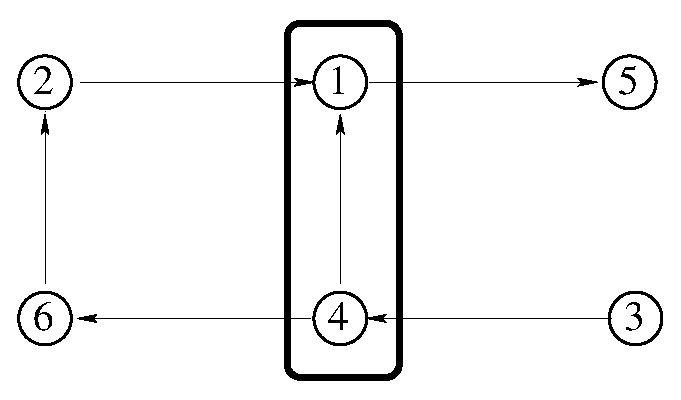
\includegraphics[width=\textwidth]{figures/matrixvertex}
% \caption{This is the second picture.}
% \label{fig:4}
\end{minipage}
}
\hfil
%\fbox
{
\begin{minipage}{.3\textwidth}
    $\left(
        \begin{array}{cc|cc|cc}
        3   & \nl & \nl & \nl & \nl   &  1  \\
        \nl & 3   &  \nl& \nl & \nl & \nl   \\ \hline
        \nl &  \nl& 3   & \nl &  1 & \nl \\
        \nl & \nl &  1 &  2  & \nl   & \nl \\ \hline
        \nl  & 1  & \nl & \nl & 2   & \nl   \\
        \nl   & \nl & \nl & 1   & 3 & 4   
        \end{array}
    \right)$
\end{minipage}
}
\end{minipage}
}
\caption{A $2$-way partition with vertex separator $V_s=\{1,4\}$
and the associated reordered matrix placing the two rows and columns associated 
with $V_s$ to the end.}\label{fig:matrixvertex}
\end{figure}

Since a naive approach to compute a recursive graph bisection is 
typically computationally expensive,
combinatorial multilevel graph bisection has been used to
accelerate the process. The basic structure is simple. The multilevel approach
consists of three phases: at first there is a coarsening phase
which compresses the given graph successively
level by level by about half of its size. When the coarsest graph with about
a few hundred vertices is reached, the second phase,  namely the so-called
bisection is applied. This is a high quality partitioning algorithm.
After that, during the uncoarsening phase, the given
bisection is successively refined as it is prolongated towards the original
graph. 

\subsubsection*{Coarsening Phase}
The initial graph $G_0=(V_0,E_0)=G(A)$ of $A\in\R^{n,n}$ is transformed during
the coarsening phase
into a sequence of graphs $G_1, G_2, \ldots, G_m$ of decreasing size 
such that $|V_0|\gg|V_1|\gg|V_2|\gg\cdots\gg|V_m|$. 
Given the graph $G_i=(V_i,E_i)$, the
next coarser graph $G_{i+1}$ is  obtained from $G_i$ by collapsing adjacent
vertices. This can be done e.g. by using a maximal matching $\cM_i$ of $G_i$ (cf. Definitions \ref{def:matching} and \ref{def:maxmatching}).
Using $\cM_i$, the next  coarser graph $G_{i+1}$ is 
constructed from $G_i$ collapsing the vertices 
being matched into multinodes, i.e., the elements of  $\cM_i$ together with the
unmatched vertices of $G_i$ become the new vertices $V_{i+1}$ of $G_{i+1}$. 
The new edges $E_{i+1}$ are the remaining edges from $E_i$ 
connected with the collapsed vertices. 
There are various differences in the construction of maximal matchings
(\cite{karypis:98,CheP08}).
One of the most popular and efficient methods is heavy edge
matching (\cite{karypis:98}).

\subsubsection*{Partitioning Phase}
At the coarsest level $m$,
a $2$-way partitioning $V_{m,1}\dot{\cup}V_{m,2}=V_m$ of $G_m=(V_m,E_m)$ is computed,
each of them containing about half of the vertices of $G_m$.
This specific partitioning of $G_m$ can be obtained by using various
algorithms such as spectral bisection (\cite{fiedler:75}) or
combinatorial methods based on Kernighan-Lin variants
(\cite{KerL70,FidM97}). It is demonstrated in \cite{karypis:98} that
for the coarsest graph, combinatorial
methods typically compute smaller edge-cut separators compared with
spectral bisection methods. However, since
the size of the coarsest graph $G_m$ is small (typically $|V_m|<100)$, this
step is negligible with respect to the total amount of computation time.

\subsubsection*{Uncoarsening Phase}
Suppose that at the coarsest level $m$, an edge separator $E_{m,s}$ 
of $G_m$ associated with the  $2$-way partitioning has been computed 
that has lead to a sufficient edge-cut of $G_m$ with $V_{m,1}$, $V_{m,2}$
of almost equal size.
Then $E_{m,s}$ is prolongated to $G_{m-1}$ by reversing the process of
collapsing matched vertices. This leads to an initial edge separator
$E_{m-1,s}$ for $G_{m-1}$. But since $G_{m-1}$ is finer, $E_{m-1,s}$ is 
sub-optimal and one usually decreases the edge-cut of the partitioning
by local refinement heuristics such as the
Kernighan-Lin partitioning algorithm (\cite{KerL70})
or the Fiduccia-Mattheyses method (\cite{FidM97}).
Repeating this refinement procedure level-by-level we obtain a sequence
of edge separators $E_{m,s},E_{m-1,s},\dots,E_{0,s}$ and eventually and
edge separator $E_{s}=E_{0,s}$ of the initial graph $G(A)$ is obtained.
If one is seeking for a vertex separator $V_s$ of $G(A)$, then one usually 
computes $V_s$ from $E_s$ at the end.

There have been a number of methods that are used for graph partitioning,
e.g. \metis{}~(\cite{karypis:98}), a parallel MPI version \parmetis{}~(\cite{KarSK99}),
or a recent multithreaded approach \mtmetis~(\cite{LasK13}).
Another example for a parallel partitioning algorithm is \scotch~(\cite{CheP08}).

\begin{example}{Multilevel Nested Dissection}\label{exm:west0479-metis}
We will continue Example \ref{exm:west0479-match} using the matrix
$\tilde A=\Pi^TD_rAD_s$ that has been rescaled and permuted using
maximum weight matching. We illustrate in Figure \ref{fig:metis} 
how multilevel nested dissection changes the pattern $\hat A=P^T \tilde A P$,
where $P$ refers to the permutation matrix associated with the partitioning
of $G(\tilde A)$.
\end{example}
\begin{figure}
%\sidecaption
\begin{minipage}{.55\textwidth}
  \begin{center}
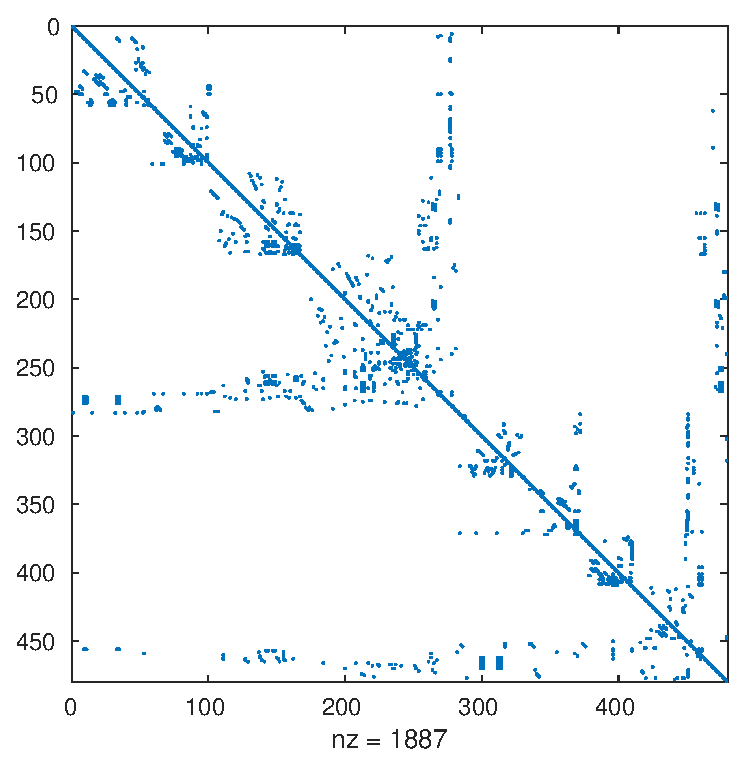
\includegraphics[width=0.95\textwidth]{figures/west0479-match-metis} 
 \end{center}  
\end{minipage}
    \caption{Application of multilevel
nested dissection after the matrix is already rescaled and permuted using maximum weight matching.}
    \label{fig:metis}
\end{figure}

%\subsection{Other reordering methods}
%One of the first methods to reorder the system was the
%reverse Cuthill-McKee (\rcm)  methods \cite{cm:69,LiuS76} which attempts
%to reduce the bandwidth of a given matrix. Though this algorithm is still 
%attractive for sequential methods and incomplete factorization methods, its use
%for direct solvers is considered as obsolete. An attractive alternative to 
%nested dissection as reordering method for direct factorization methods is
%the minimum degree algorithm (\mmd) \cite{Ros72,GeoL89} and its recent variants,
%in particular the approximate minimum degree algorithm (\amd) \cite{AmeDD96,Dav06} 
%with or without constraints. The main objective of the minimum degree algorithm
%is to simulate the Gaussian elimination process symbolically by investigating
%the update process $a_{ij}\to a_{ij}-a_{ik}a_{kk}^{-1}a_{kj}$ by means of graph
%theory, at least in the case of the undirected graph. 
%The name-giving degree refers to the number of edges connected to a vertex and 
%how the graph and therefore the degrees of its vertices change during the 
%factorization process.
%Over the years this
%has lead to an evolution of the underlying minimum degree algorithm
%using the so-called \emph{external degree} for selecting vertices as pivots
%and  
%further techniques like \emph{incomplete degree update}, 
%\emph{element absorption} and \emph{multiple elimination} 
%as well as data structures based on cliques. 
%For an overview see \cite{GeoL89}.
%One of the most costly parts in the minimum degree algorithm  is to update
%of the degrees. Instead of computing the exact external degree, in
%the approximate minimum degree algorithm
%\cite{AmeDD96} an approximate external degree is computed that significantly
%saves time while producing comparable fill in the $LU$ decomposition.
%
%We like to conclude this section by mentioning that if nested dissection is computed
%to produce a vertex separator $V_s$ and a related $k$-way partitioning $V_1,\dots,V-k$ for the remaining vertices of $V\setminus V_s$ of $G(A)=(V,E)$ 
%which allow for parallel
%computations, then the entries of each $V_i$, $i,\dots,k$ could be taken in
%any order. Certainly, inside $V_i$ one could use nested dissection as well, which
%is the default choice in multilevel nested dissection methods. However, as soon
%as the coarsest graph $G_m$ is small enough (typically about $100$ vertices),
%not only the separator is computed, but in addition the remaining entries of
%$G_m$ are reordered to lead to a fill-reducing ordering. In both cases, for
%$G_m$ as well as $V_1,\dots,V_k$ one could alternatively use different reordering
%methods such as variants of the minimum degree algorithm. Indeed, for
%$G_m$ this is what the \metis software is doing. Furthermore, a reordering
%method such as the constrained approximate minimum degree algorithm is also
%suitable as local reordering for $V_1,\dots,V_k$ as alternative to nested 
%dissection, taking into account the edges connected with $V_s$ (also referred to
%as HALO structure), see e.g. \cite{PelRA00}.


\section{Sparse $LU$ Factorization \todol{ldl instead}}
\label{sec:lu}
In this section we will assume that the given matrix $A\in\R^{n,n}$ is nonsingular and that it can be factorized as $A=LU$, where $L$ is a lower triangular matrix with unit diagonal and
$U$ is an upper triangular matrix. 
It is well-known (\cite{GeoL81}), if $A=LU$, where $L$ and $U^\top$ are lower
triangular matrices, then in the generic case we will have
$G_d(L+U)\supset G_d(A)$, i.e., we will only get additional edges unless some
entries cancel by ``accident'' during the elimination. In the sequel
we will ignore cancellations. Throughout this section we will always assume
that the diagonal entries of $A$ are nonzero as well. We also assume that $G_d(A)$
is connected.


In the preceding sections we have argued that
maximum weight matching often leads to a rescaled and reordered matrix such that
static pivoting is likely to be enough, i.e., 
pivoting is restricted to some dense blocks inside the $LU$ factorization.
Furthermore, reordering strategies such as multilevel nested dissection have 
further symmetrically permuted the system such that the fill-in that occurs
during Gaussian elimination is acceptable and even parallel approaches could
be drawn from this reordering. Thus assuming that $A$ does not need further
reordering and a factorization $A=LU$ exists 
is a realistic scenario in what follows.




%We begin with some basic terminology. 
%For a matrix $A=\left(a_{ij}\right)_{i,j=1,\dots,n}\in\R^{n,n}$ we denote by $A_{k:l,p:q}$ the submatrix $\left(a_{ij}\right)_{i=k,\dots,l, j=p,\dots,q}$ of $A$. Here we always assume that $1\leqslant k\leqslant l\leqslant n$ and $1\leqslant p\leqslant q\leqslant n$. 
% Next we introduce some definitions from graph theory associated with a given matrix $A\in\R^{n,n}$.
%\begin{definition}
%For a matrix $A\in\R^{n,n}$ we
% define the associated graph $G(A)$ by the pair $(V,E)$, where 
%$V=\{1,\dots,n\}$ and the set of edges 
%$E=\left\{(i,j):\, a_{ij}\not=0\right\}$.
%\end{definition}
% Whenever we refer to an \emph{undirected} graph we mean that $(i,j)\in G(A)$ if and only if $(j,i)\in G(A)$. In this case we may also use $\{i,j\}$ instead of $(i,j)$.


\subsection{The Elimination Tree}
\label{subsec:etree}
% We assume that our matrix $A$ possesses an $LU$ decomposition (see e.g \cite{GolV96}). 
The basis of determining the fill-in in the triangular factors 
$L$ and $U$ as by-product of the Gaussian elimination can be characterized
as follows (see \cite{Gil94} and the references therein). 

\begin{theorem}\label{thr:gilbert}
Given $A=LU$ with the aforementioned assumptions, 
there exists an edge $(i,j)$ in $G_d(L+U)$ if and only if there exists a path
\[
ix_1, x_2x_3, \dots, x_kj
\]
in $G_d(A)$ such that $x_1,\dots,x_k<\min(i,j)$.
\end{theorem}
In other words, during Gaussian elimination we obtain a fill edge $(i,j)$ for
every path from $i$ to $j$ through vertices less than $\min(i,j)$.

\begin{example}{Fill-in}\label{exm:fill}
We will use the matrix $\Pi^TA$ from Example \ref{exm:vsep}  and sketch
the fill-in obtained during Gaussian elimination   in Figure \ref{fig:fill}.
\end{example}
\begin{figure}
%\sidecaption
\begin{minipage}{.45\textwidth}
    $\left(
        \begin{array}{cc|cc|cc}
        3   & \nl & \nl & \nl & \nl   &  1  \\
        \nl & 3   &  \nl& \nl & \nl & \nl   \\ \hline
        \nl &  \nl& 3   & \nl &  1 & \nl \\
        \nl & \nl &  1 &  2  & \times   & \nl \\ \hline
        \nl  & 1  & \nl & \nl & 2   & \nl   \\
        \nl   & \nl & \nl & 1   & 3 & 4   
        \end{array}
    \right)$
\end{minipage}
    \caption{Fill-in with respect to $L+U$ is denoted by $\times$.}
    \label{fig:fill}
\end{figure}

% As usual we will denote directed edges $(i,j)$ by an arrow whereas if $(i,j)$ and $(j,i)$ exist we omit the arrow and just draw a line (see Figure \ref{matrixpattern}). 
%\begin{definition}
%Let $A\in\R^{n,n}$. For an edge $(i,j)$ in $G(A)$ we will write 
%$i\stackrel{G(A)}{\to} j$ or simply  $i{\to} j$ if the graph is
%clear from the context. Likewise we will write
%$i\stackrel{G(A)}{\Rightarrow} j$ or simply  $i{\Rightarrow} j$ if the
%exists a path from $i$ to $j$ in $G(A)$.
%\end{definition}

The fastest known method for predicting the filled graph $G_d(L+U)$ is Gaussian elimination. 
The situation is simplified if the
 graph is undirected. 
In the sequel we ignore the orientation of the edges and simply consider
the undirected graph $G(A)$ and $G(L+U)$, respectively.

\begin{definition}\label{def:filled-graph}
The undirected graph $G(L+U)$ that is derived from the undirected graph 
$G(A)$ by applying Theorem \ref{thr:gilbert} is called the filled graph
and it will be denoted by $G_f(A)$.
\end{definition}


%\begin{example}{Fill-in with respect to the undirected graph}\label{exm:symfill}
%When we consider the undirected graph $G(A)$ in Example \ref{exm:fill},
%the pattern of $|\Pi^TA|+|\Pi^TA|^T$ and its filled graph $G_f(A)$ now equals 
%$G(A)$ up to positions $(5,4)$ and $(4,5)$
%(cf. Figure \ref{fig:symfill}).
%\end{example}
%\begin{figure}
%%\sidecaption
%\begin{minipage}{.45\textwidth}
%    $\left(
%        \begin{array}{cc|cc|cc}
%         \bullet & \nl     &  \nl    &   \nl   &  \nl    & \bullet \\
%         \nl     & \bullet &  \nl    &   \nl   & \bullet & \nl     \\ \hline
%         \nl     & \nl     & \bullet & \bullet & \bullet & \nl     \\
%         \nl     & \nl     & \bullet & \bullet & \times  & \bullet \\ \hline
%         \nl     & \bullet & \bullet & \times  & \bullet & \bullet \\
%         \bullet & \nl     &  \nl    & \bullet & \bullet & \bullet   
%        \end{array}
%    \right)$
%\end{minipage}
%    \caption{Entries of $G(A)$ are denoted by $\bullet$, fill-in is denoted by $\times$.}
%    \label{fig:symfill}
%\end{figure}
%
%The key tool to predict the fill-in easily for the undirected graph is the
%\emph{elimination tree} \cite{Liu90}. 
%
%Recall that an undirected and connected
%graph is called a \emph{tree}, if it does not contain any cycle.
%Furthermore, one vertex is identified as \emph{root}.
%As usual we call a vertex $j$ \emph{parent} of $i$, if there exists an edge
%$(i,j)$ in the tree such that $j$ is closer to the root. In this case
%$i$ is called \emph{child} of $j$. The subtree rooted at vertex $j$ is denoted
%by $T(j)$ and the vertices of this subtree 
%are called \emph{descendants} of $j$ whereas $j$ is called their \emph{ancestor}.
%%
%Initially we will define the elimination tree algorithmically 
%using the depth-first-search algorithm \cite{AhoHU83}. Later we will
%state a much simplified algorithm. 
%\begin{definition}\label{def:etree}
%Given the filled graph $G_f(A)$ the
%\emph{elimination tree} $T(A)$ is defined by the following algorithm.\\
%Perform a depth-first-search in $G_f(A)$ starting
%from vertex $n$.\\  
%When vertex $m$ is visited, choose
%from its unvisited neighbors $i_1,\dots,i_k$ the index
%$j$ with the largest number $j=\max\{i_1,\dots,i_k\}$ and
%continue the search with $j$. \\
%A leaf of the tree is reached, 
%when all neighbors have already been visited.
%\end{definition}
%We like to point out that the application of the 
%depth-first-search to $G_f(A)$ starting at vertex $n$ behaves
%significantly different from other graphs.
%By Theorem \ref{thr:gilbert} it follows that
%as soon as we visit a vertex $m$, all its neighbors $j>m$ must have been 
%visited prior to vertex $m$. Thus  the labels of the vertices are strictly 
%decreasing until we reach a leaf node.
%% maybe another simple examples for graphs which cannot be G_f(A)
%% 1-2-3 ok, 2-1-3 not ok,  1-2 not ok
%%                          | |
%%                          4-3
%
%\begin{example}{Depth-first-search}\label{exm:dfs}
%We illustrate the depth-first-search using the (filled) graph in
%Figure \ref{fig:matrixpattern} and the pattern from Example \ref{exm:symfill}.
%The extra fill edge is marked by a bold line. 
%
%The ongoing depth-first search visits the vertices in the order
%$6\to5\to4\to 3$. Since at vertex $3$, all neighbors of $3$ are visited (and indeed have a larger number), the algorithm backtracks to $4$ and to $5$ and continues the search in the order
%$5\to2$. Again all neighbors of vertex $2$ are visited (and have larger number), 
%thus the algorithm backtracks to $5$ and to $6$ and continues by $6\to1$. Then the
%algorithm terminates.
%% Note that vertex $3$ is isolated and if the graph of $A$ is not connected one has to proceed for each connected component separately.
%\end{example}
%\begin{figure}[htb]
%%\sidecaption
%%\fbox
%{
%\begin{minipage}{.35\textwidth}
%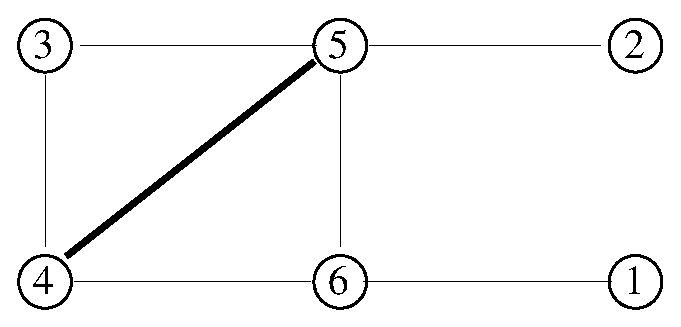
\includegraphics[width=\textwidth]{figures/filledgraph}
%\end{minipage}
%}
%~~~~\hfil~~~~
%%\fbox
%{
%\begin{minipage}{.5\textwidth}
%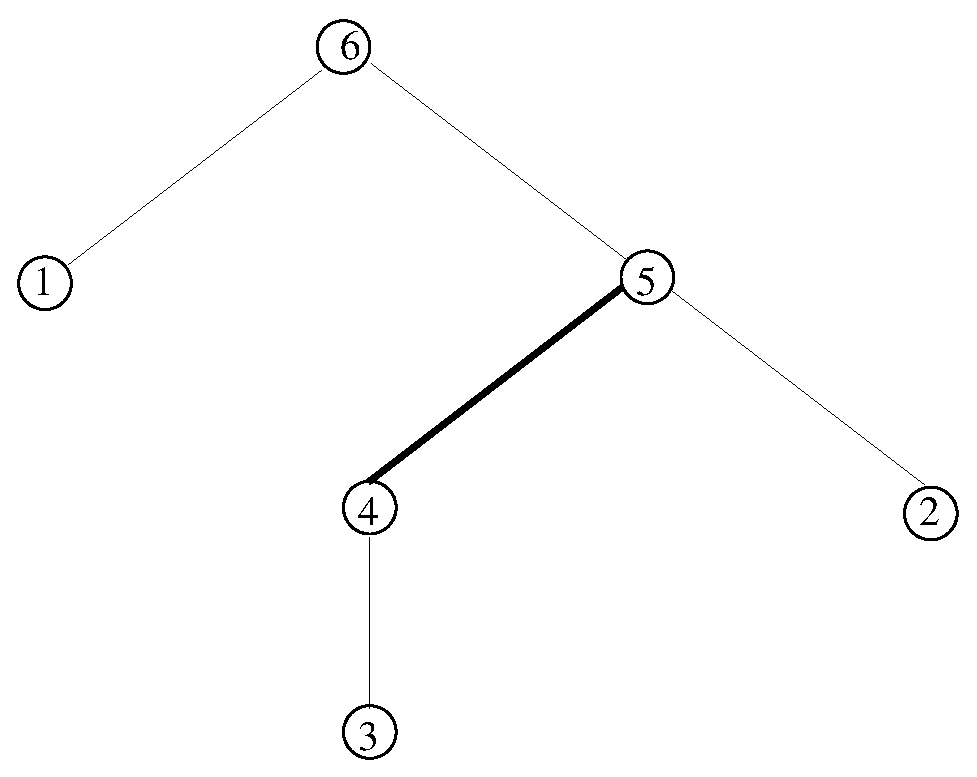
\includegraphics[width=\textwidth]{figures/etree}
%\end{minipage}
%}
%\caption{Filled graph (left) and elimination tree (right).}\label{fig:matrixpattern}
%\end{figure}
%

\begin{remark}\label{rem:cross-edges}
It follows immediately from the construction of elimination tree $T(A)$ and Theorem
\ref{thr:gilbert}
that additional edges of $G_f(A)$ which are not covered by the elimination
tree can only show up between a vertex and some of its ancestors (referred to as ``back-edges''). In contrast to that, ``cross-edges'' between unrelated vertices
do not exist.
\end{remark}

\begin{remark}\label{rem:dependence}
One immediate consequence of Remark \ref{rem:cross-edges} is
that triangular factors can be computed independently starting from the
leaves until the vertices meet a common parent, i.e.,
column $j$ of $L$ and $U^T$ only depend on those columns $s$
of $L$ and $U^T$ such that $s$ is a descendant
of $j$ in the elimination tree $T(A)$.
\end{remark}

\begin{example}{Elimination tree}\label{exm:etree}
We use the matrix ``west0479'' from Example \ref{exm:west0479-metis},
after maximum weight matching and multilevel nested dissection have
been applied. We use \ml's \texttt{etreeplot} to display its elimination
tree (see Figure \ref{fig:etreeplot}). The elimination tree displays the high
level of concurrency that is induced by nested dissection, since 
by Remark \ref{rem:dependence} the computations can be executed independently
at each leaf node towards the root until a common parent vertex is reached.
\end{example}
\begin{figure}
%\sidecaption
%\fbox
{
\begin{minipage}{.99\textwidth}
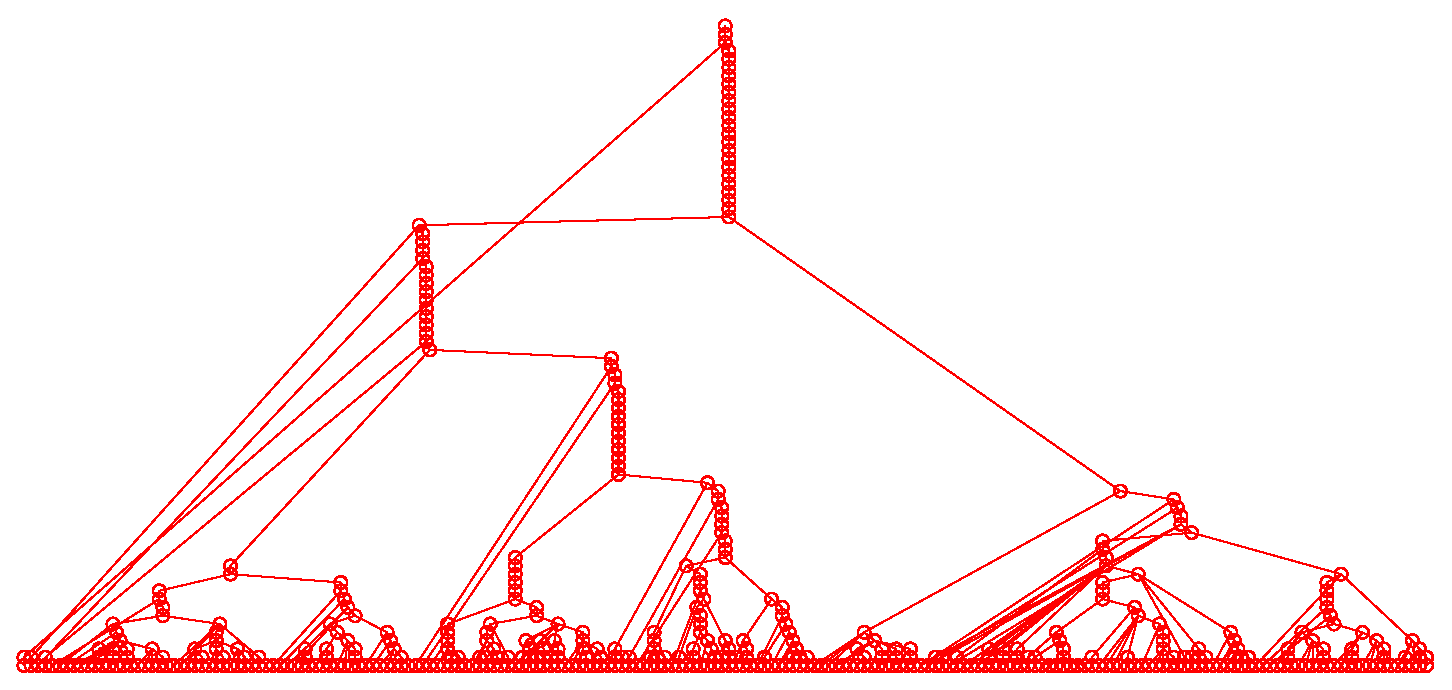
\includegraphics[width=\textwidth,height=0.3\textwidth]{figures/west0479-match-metis-etree}
\end{minipage}
}
\caption{Elimination tree of ``west0479'' after maximum weight matching and nested dissection are applied.}\label{fig:etreeplot}
\end{figure}





Further conclusions can be easily derived
from the elimination tree, in particular
Remark   \ref{rem:dependence} in conjunction with Theorem \ref{thr:gilbert}.
\begin{remark}\label{rem:path-compression}
Consider some $k\in\{1,\dots,n\}$. Then there exists a (fill) edge $(j,k)$
with $j<k$ if and only if there exists a common
descendant $i$ of $k,j$ in $T(A)$ such that $a_{ik}\not=0$.
This follows from the fact that once $a_{ik}\not=0$, by Theorem \ref{thr:gilbert}
this induces (fill) edges $(j,k)$ in the filled graph $G_f(A)$ for all nodes
$j$ between $i$ and $k$ in the elimination tree $T(A)$, i.e., for all ancestors
of $i$ that are also descendants of $k$. This way, $i$ propagates fill-edges
along the branch from $i$ to $k$ in $T(A)$ and the information $a_{ik}\not=0$ can be
used as path compression to advance from $i$ towards $k$ along the elimination
tree.
\end{remark}
%\begin{example}{Path compression}\label{exm:pc}
%Consider the graph and the elimination tree from 
%Figure \ref{fig:matrixpattern}. Since there exists the edge $(3,5)$ in $G(A)$,
%therefore another (fill) edge $(4,5)$ must exist. Similarly, the same conclusion can be drawn
%from the existence of the edge $(4,6)$ (here not a fill edge, but a regular edge).
%\end{example}
%
%
%The elimination tree itself can be easily described by a vector $p$ of length
%$n$ such that for any $i<n$, $p_i$ denotes the parent node while $p_n=0$
%corresponds to the root. 
%Consider some step $k$ with $a_{ik}\not=0$, for some $i<k$. 
%By Remark \ref{rem:path-compression}, $i$ must be a descendant of $k$
%and there could be further ancestors $j$ of $i$ which are also descendants of $k$.
%Possibly not all ancestors of $i$ have been assigned a parent node so far.
%Thus we can replace $i$ by $j=p_i$ until we end up with $p_j=0$ or $p_j\geqslant k$.
%This way we traverse $T(A)$ from $i$ towards to $k$ until we have found the child 
%node $j$ of $k$. If the parent of $j$ has not been assigned to $j$ yet, 
%then $p_j=0$ and $k$ must be the parent of $j$. If some $l<k$ were the parent of 
%$j$, then we would have assigned $l$ as parent of $j$ in an earlier step $l<k$.
%In this case we set $p_j\leftarrow k$. Otherwise, if $p_j\geqslant k$, then we have already
%assigned $j$'s parent in an earlier step $l<k$.
%
%\begin{example}{Computation of parent nodes}\label{exm:parent_nodes}
%Consider the elimination tree $T(A)$ from Figure \ref{fig:matrixpattern}.
%Unless $k=4$, no parents have been assigned, i.e. $p_i=0$ for all $i$.
%
%Now for $k=4$ we have 
%$a_{34}\not=0$ and using the fact that $p_3=0$ implies that we have to set
%$a_3=p_3\leftarrow 4$.
%
%For $k=5$, 
%$a_{25}\not=0$ and again $p_2=0$ requires to set $a_2=p_2\leftarrow 5$.
%Next, $a_{35}\not=0$, path compression enables $a_3\leftarrow 5$ and
%after another loop we obtain $a_4=p_4\leftarrow 5$.
%
%Finally, if $k=6$, we have $a_{16}\not=0$
%and immediately obtain $a_1=p_1\leftarrow 6$.
%Since $a_{46}\not=0$,  a path compression is applied  which yields
%$a_4\leftarrow 6$ and in the next step we set $a_5=p_5\leftarrow 6$.
%At last $a_{56}\not=0$ does not cause further changes.
%
%In total we have $p=[6, 5, 4, 5, 6, 0]$ which perfectly reveals the parent
%properties of the elimination trees in  Figure \ref{fig:matrixpattern}.
%\end{example}
%
%By Remark \ref{rem:path-compression} (cf. \cite{Tar83,Dav06}), 
%we can also make use of path compression.
%Since our goal is to traverse the branch of the elimination tree from $i$ to $k$
%as fast as possible, any ancestor $j=a_i$ of $i$ would be sufficient. With the
%same argument as before, an ancestor $a_j=0$ would refer to a vertex that does
%not have a parent yet. In this case we can again set $p_j\leftarrow k$. Moreover,
%$k$ is always an ancestor of $a_i$.
%
%
%
%
%The algorithm including path compression can be summarized as follows 
%(see also  \cite{Liu90,Dav06}).
%\begin{programcode}{Computation of the elimination tree}\label{alg:etree}
%\begin{algorithmic}[1]
%  \Require $A\in\R^{n,n}$ such that $A$ has the same pattern as $|A|+|A|^T$.
%  \Ensure vector $p\in\R^n$ such that $p_i$ is the parent of $i$, $i=1,\dots,n-1$,
%except $p_n=0$.
%  \State let $a\in\R^n$ be an auxiliary vector used for path compression.
%  \State $p\leftarrow 0, a\leftarrow 0$
%    \For{$k=2,\dots,n$}
%        \For{all $i<k$ such that $a_{ik}\not=0$}
%            \While{$i\not=0$ and $i<k$}
%                  \State $j\leftarrow a_i$
%                  \State $a_i\leftarrow k$
%                  \If{$j=0$} 
%                     \State $p_i\leftarrow k$
%                  \EndIf   
%                  \State $i\leftarrow j$
%            \EndWhile
%        \EndFor
%    \EndFor
%\end{algorithmic}
%\end{programcode}




\subsection{The supernodal factorization approach}
We have already seen that the elimination tree reveals information about
concurrency. It is further useful to determine the fill-in $L$ and $U^T$.
This information can be computed from the elimination tree $T(A)$ together
with $G(A)$. The basis for determining the fill-in in each column is 
again Remark \ref{rem:path-compression}. Suppose we are interested in the
nonzero entries of column $j$ of $L$ and $U^T$. Then for all descendants of $j$,
i.e. the nodes of the subtree $T(j)$ rooted at vertex $j$, a nonzero entry
$a_{ik}\not=0$ also implies $l_{kj}\not=0$. Thus, starting at any leaf $i$,
we obtain its fill by all $a_{ik}\not=0$ such that $k>i$ and when we move forward
from $i$ to its parent $j$, vertex $j$ will inherit the fill from node $i$ for
all $k>j$ plus the nonzero entries given by $a_{jk}\not=0$ such that $k>j$.
When we reach a common parent node $k$ with multiple children, the same argument
applies using the union of fill-in greater than $k$ from its children together
with the nonzero entries $a_{kl}\not=0$ such that $l>k$.
We summarize this result in a very simple algorithm
\begin{programcode}{Computation of fill-in}\label{alg:compute_pattern}
\begin{algorithmic}[1]
  \Require $A\in\R^{n,n}$ such that $A$ has the same pattern as $|A|+|A|^T$.
  \Ensure sparse strict lower triangular pattern $P\in\R^{n,n}$ with
  same pattern as $L$, $U^T$.
  \State compute parent array $p$ of the elimination tree $T(A)$
  \For{$j=1,\dots,n$}
      \State supplement nonzeros of column $j$ of $P$ with all $i>j$ such that $a_{ij}\not=0$ 
      \State $k=p_j$
      \If{$k>0$} 
         \State supplement nonzeros of column $k$ of $P$ with nonzeros of column $j$ of $P$ greater than $k$
      \EndIf   
  \EndFor
\end{algorithmic}
\end{programcode}



Algorithm \ref{alg:compute_pattern} only deals with the fill pattern. 
One additional aspect that allows to raise efficiency
and to speed up the numerical factorization significantly 
is to detect dense submatrices in the factorization.
Block structures  allow to collect parts
of the matrix in dense blocks and to treat them commonly using 
dense matrix kernels such as level-3 BLAS and LAPACK (\cite{DodL85,DonDHH88}).

Dense blocks can be read off from the elimination tree employing
Algorithm \ref{alg:compute_pattern}.
\begin{definition}\label{def:supernode}
Denote by $\mathcal{P}_j$ the nonzero indices of column $j$ of $P$
as computed by Algorithm \ref{alg:compute_pattern}.
A sequence $k,k+1,\dots,k+s-1$ is called supernode of size $s$
if the columns of $\mathcal{P}_{j}=\mathcal{P}_{j+1}\cup \{j+1\}$
for all $j=k,\dots,k+s-2$.
\end{definition}
In simple words, Definition \ref{def:supernode} states that for a supernode
$s$ subsequent columns can be grouped together in one dense block with a triangular
diagonal block and a dense subdiagonal block since they perfectly match the 
associated trapezoidal shape. We can thus easily supplement 
Algorithm \ref{alg:compute_pattern} with a supernode detection.
\begin{programcode}{Computation of fill-in and supernodes}\label{alg:compute_supernode}
\begin{algorithmic}[1]
  \Require $A\in\R^{n,n}$ such that $A$ has the same pattern as $|A|+|A|^T$.
  \Ensure sparse strict lower triangular pattern $P\in\R^{n,n}$ with
  same pattern as $L$, $U^T$ as well as column size $s\in\R^m$ of each supernode.
  \State compute parent array $p$ of the elimination tree $T(A)$
  \State $m\leftarrow0$ 
  \For{$j=1,\dots,n$}
      \State supplement nonzeros of column $j$ of $P$ with all $i>j$ such that $a_{ij}\not=0$ 
      \State denote by $r$ the number of entries in column $j$ of $P$
      \If{$j>1$ and $j=p_{j-1}$ and $s_m+r=l$}
         \State $s_m\leftarrow s_m+1$ \Comment{continue current supernode}
      \Else
         \State $m\leftarrow m+1$, $s_m\leftarrow 1$, $l\leftarrow r$ \Comment{start new supernode}
      \EndIf
      \State $k=p_j$
      \If{$k>0$} 
         \State supplement nonzeros of column $k$ of $P$ with nonzeros of column $j$ of $P$ greater than $k$
      \EndIf   
  \EndFor
\end{algorithmic}
\end{programcode}





\begin{example}{Supernode Computation}\label{exm:supernode_computation}
To illustrate the use of supernodes, we consider the matrix pattern
from Figure \ref{fig:symfill} and illustrate the underlying
dense block structure in Figure \ref{fig:supernode}.
Supernodes are the columns $1$, $2$, $3$ as scalar columns as well as columns
$4$-$6$ as one single supernode.
\end{example}
\begin{figure}
   \centering
   \subfloat[Undirected graph $G(A)$ represented as a matrix.]{
      $\left(
      \begin{array}{cc|cc|cc}
         \bullet & \nl     &  \nl    &   \nl   &  \nl    & \bullet \\
         \nl     & \bullet &  \nl    &   \nl   & \bullet & \nl     \\ \hline
         \nl     & \nl     & \bullet & \bullet & \bullet & \nl     \\
         \nl     & \nl     & \bullet & \bullet & \times  & \bullet \\ \hline
         \nl     & \bullet & \bullet & \times  & \bullet & \bullet \\
         \bullet & \nl     &  \nl    & \bullet & \bullet & \bullet
      \end{array}
      \right)$
      %\caption{Entries of $G(A)$ are denoted by $\bullet$, fill-in is denoted by $\times$.}
      \label{fig:symfill}
   } \, \hspace{0.5cm}
   \subfloat[Supernodes in the triangular factor.]{
      $\left(
      \begin{array}{cccccc}
         \\[-1.8ex]\cline{1-1}
         \multicolumn{1}{|c|}{\bullet}&       &       &       &       &         \\ \cline{1-2}
         \nl    &\multicolumn{1}{|c|}{\bullet}&       &       &       &         \\ \cline{2-3}
         \nl    &\nl    &\multicolumn{1}{|c|}{\bullet}&       &       &         \\ \cline{4-4}
         \nl    &\nl    & \multicolumn{1}{|c|}{\bullet}   &\multicolumn{1}{|c|}{\bullet}&       &         \\ \cline{2-2}\cline{5-5}
         \nl    &\multicolumn{1}{|c|}{\bullet}& \multicolumn{1}{|c|}{\bullet}   &\multicolumn{1}{|c}{\times}&\multicolumn{1}{c|}{\bullet}&         \\ \cline{1-3}\cline{6-6}
         \multicolumn{1}{|c|}{\bullet}&\nl& \nl   &\multicolumn{1}{|c}{\bullet}&\bullet& \multicolumn{1}{c|}{\bullet}\\
         \cline{1-1}\cline{4-6}
      \end{array}
      \right)$
      %\caption{Supernodes in the triangular factor.}
      \label{fig:supernode}
   }
   \caption{Matrix representation of an undirected graph $G(A)$ and supernodes in its triangular factor. Entries of $G(A)$ are denoted by $\bullet$, fill-in is denoted by~$\times$.}
   %\label{fig:supernode}
\end{figure}

Supernodes form the basis of several improvements, e.g.,
a supernode can be stored as one or two dense matrices. 
Beside the storage scheme as dense matrices, the nonzero row indices
for these blocks need only be stored once.
Next the use of dense submatrices allows the usage of dense matrix kernels
using level-3 BLAS
(\cite{DodL85,DonDHH88}).
\begin{example}{Supernodes}\label{exm:supernodes}
We use the matrix ``west0479'' from Example \ref{exm:west0479-metis},
after maximum weight matching and multilevel nested dissection have
been applied. 
We use its undirected graph to compute the supernodal
structure. Certainly, since the matrix is nonsymmetric, the block structure
is only sub-optimal. We display the supernodal structure for the associated
Cholesky factor, i.e., for the Cholesky factor of a symmetric positive definite
matrix with same undirected graph as our matrix (see
left part of Figure \ref{fig:supernodal_structure}). Furthermore, we display
the supernodal structure for the factors $L$ and $U$ computed from the
nonsymmetric matrix without pivoting (see right part of Figure \ref{fig:supernodal_structure}).
\end{example}
\begin{figure}
% \sidecaption
\begin{minipage}{.48\textwidth}
 \begin{center}
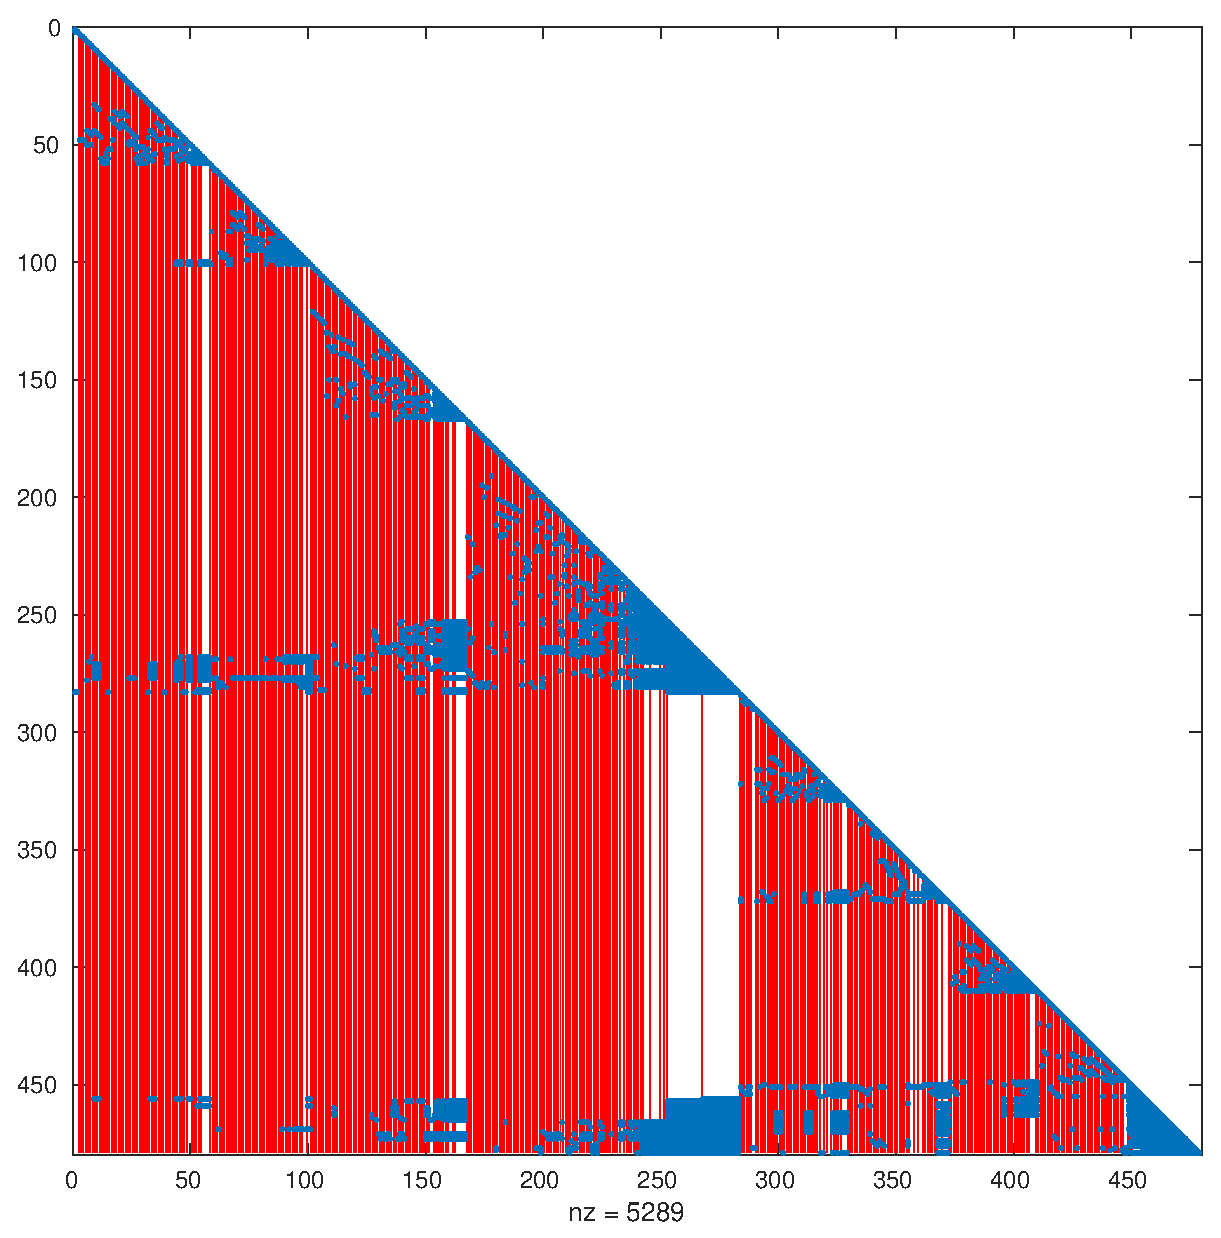
\includegraphics[width=0.99\textwidth]{figures/west0479-match-metis-chol-super} 
 \end{center}
\end{minipage}
~
\begin{minipage}{.48\textwidth}
  \begin{center}
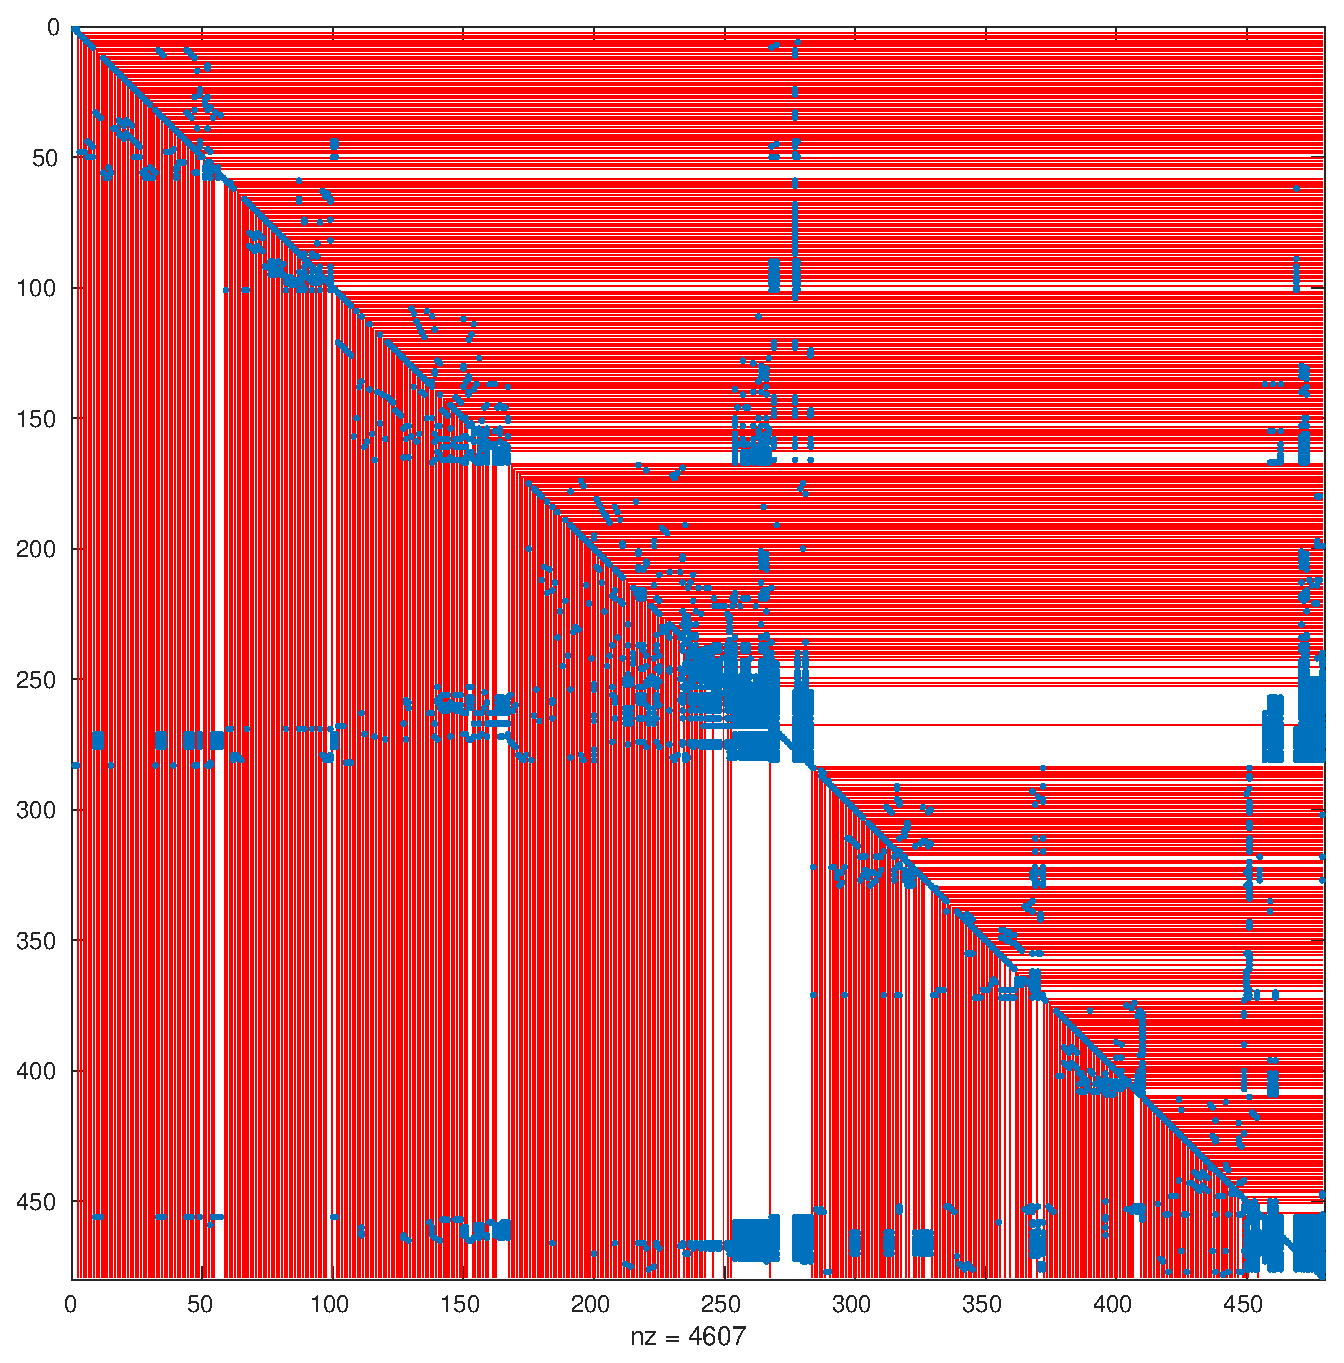
\includegraphics[width=0.99\textwidth]{figures/west0479-match-metis-lu-super} 
 \end{center}  
\end{minipage}
    \caption{Supernodal structure. Left: vertical lines display the blocking of the
supernodes with respect to the associated Cholesky factor. Right: 
vertical and horizontal lines display the blocking of the
supernodes applied to $L$ and $U$.}
    \label{fig:supernodal_structure}
\end{figure}

While the construction of supernodes is fairly easy in the symmetric case,
its generalization for the nonsymmetric case is significantly harder, since one
has to deal with pivoting in each step of Gaussian elimination.
In this case one uses the column elimination tree (\cite{GeoN85}).

\section{Supernodal Data Structures}
%%%\label{sec:BLAS3}
\label{sec:parallel}

High-performance sparse solver libraries have been a very important part of
scientific and engineering computing for years, and their importance
continues to grow as microprocessor architectures become more complex
and software libraries become better designed to integrate easily
within applications. Despite the fact that there are various science
and engineering applications, the underlying algorithms typically have
remarkable similarities, especially those algorithms that are most
challenging to implement well in parallel. It is not too strong a
statement to say that these software libraries are essential to the
broad success of scalable high-performance computing in computational
sciences.  In this section we demonstrate the benefit of supernodal data structures within the 
sparse solver package PARDISO~(\cite{schenk-2004}). We illustrate it by using
the triangular solution process. The forward and backward substitution is performed
column wise with respect to the columns of $L$, starting with the
first column, as depicted in Figure~\ref{algo:triangular}.
The data dependencies here allow to store vectors $y$, $z$, $b$, and $x$ in only one
vector $r$. When column $j$ is reached, $r_j$ contains the solution for $y_j$. 
All other elements of $L$ in this column, i.\,e.\ $L_{ij}$ with $i = j + 1,
\ldots, N$, are used to update the remaining entries in $r$ by 
%
\be
  r_i = r_i - r_j L_{ij}.
  \label{eq:algo:fw:pardiso}
\ee
%
The backward substitution with~$L^T$ will take place row wise, since we
use $L$ and perform the substitution column wise with respect to $L$, as shown in the lower part of
Figure~\ref{algo:triangular}.  In contrast to the forward substitution the
iteration over columns starts at the last column $N$ and proceeds to
the first one.  If column $j$ is reached, then $r_j$, which contains the $j$-component of the solution vector $x_j$,
is computed by subtracting the dot-product of the remaining elements in
the column $L_{ij}$ and the corresponding elements of $r_i$ with $i =
j + 1, \ldots, N$ from it:
%
\be
  r_j = r_j - r_i L_{ij} .
  \label{eq:algo:bw:pardiso}
\ee
%
After all columns have been processed $r$ contains the required solution $x$. It is important to note that
line 5 represents in both substitutions an indexed DAXPY and indexed
DDOT kernel operations that has to be computed during the streaming 
operations of the vector $r$ and the column $j$ of the numerical factor $L$. 
As we are dealing with sparse matrices it makes no sense to store the lower
triangular matrix $L$ as a dense matrix.
Hence PARDISO uses its own data structure to store $L$, as shown in
Figure~\ref{fig:algo:ds}. 
%
\begin{figure*}[t]
    \centering
    \begin{minipage}{.35\textwidth}
        \centering
        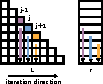
\includegraphics[width=0.85\textwidth,clip=true]{images/forward-small}
    \end{minipage}%
    \begin{minipage}{0.65\textwidth}
        \centering
  \begin{algorithmic}[1]
    \Procedure{Sparse forward substitution}{}
            \For{j = 0; j < n; j++}\label{algo:fw:cholmod}
                \For{i = \nxlnz[j]; i < \nxlnz[j+1]; i++}
                   \State row = \nindx[i]
                   \State \nr[row] -=  \nr[j] * \nlnz[i] \Comment{indexed DAXPY}
            \EndFor\label{algo:fw:cholmod:rloop:end}
      \EndFor
    \EndProcedure
  \end{algorithmic}
    \end{minipage}

\bigskip

    \centering
    \begin{minipage}{.35\textwidth}
        \centering
        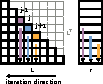
\includegraphics[width=0.85\textwidth,clip=true]{images/backward-small}
    \end{minipage}%
    \begin{minipage}{0.65\textwidth}
        \centering
  \begin{algorithmic}[1]
    \Procedure{Sparse backward substitution}{}
            \For{j =  n;  j > 0; j - -}\label{algo:bw:cholmod}
                \For{i = \nxlnz[j]; i < \nxlnz[j+1]; i++}
                   \State row = \nindx[i]
                   \State \nr[j] -=  \nr[row] * \nlnz[i] \Comment{indexed DDOT}
            \EndFor\label{algo:bw:cholmod:rloop:end}
      \EndFor
    \EndProcedure
  \end{algorithmic}
    \end{minipage}
  \caption{Sparse triangular substitution in CSC format based on indexed DAXPY/DDOT kernel operations.}
  \label{algo:triangular}
\end{figure*}


\begin{figure}[t]
  \centering
    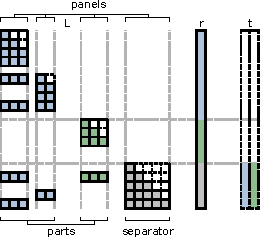
\includegraphics[width=0.5\textwidth,clip=true]{images/parts-panels-separator}
  \caption{Sparse matrix data structures in PARDISO. Adjacent columns of $L$ exhibiting the same
structure form panels also known as supernodes. 
Groups of panels which touch independent elements of the right hand side $r$ are
parts. The last part in the lower triangular matrix $L$ is called separator.}
  \label{fig:algo:ds}
\end{figure}


%\begin{algorithm}[t]
%  \begin{algorithmic}[1]
%    \Procedure{Forward}{}
%      \For{part $o$ in parts} \Comment{parallel execution}
%        \For{panel p in part $p$}
%          \For{\textcolor{blue}{column $j$ in panel}} \Comment{unroll} \label{alg:fw:1}
%            \State i = \nxindx{}[p] + offset
%
%            \For{k = \nxlnz[j] + offset; k < sep; ++k}\label{algo:fw:rloop}
%                \State row = \nindx[i++]
%                \State \nr[row] - =  \nr[j] \nlnz[k] \Comment{indexed DAXPY}
%            \EndFor\label{algo:fw:rloop:end}
%            \For{k = sep + 1; k < \nxlnz[j+1]; ++k}\label{algo:fw:seploop}
%                \State row = \nindx[i++]
%                \State \ntemp[row,p] -=  \nr[j] \nlnz[k] \Comment{indexed DAXPY}
%            \EndFor\label{algo:fw:seploop:end}
%          \EndFor
%        \EndFor
%      \EndFor
%      \State r[i] = r[i] - sum(\ntemp[i,:])  \Comment{gather temporary arrays}
%      \For{panel p in separator} \Comment{serial execution}
%        \For{\textcolor{blue}{column $j$ in panel}} \Comment{unroll}\label{alg:fw:2}
%            \State i = \nxindx[p] + offset
%
%            \For{k = \nxlnz[j] + offset; k < \nxlnz[j+1]; ++k}
%                \State row = \nindx[i++]
%                \State \nr[row] -=  \nr[j] \nlnz[k] \Comment{indexed DAXPY}
%            \EndFor
%        \EndFor
%      \EndFor
%    \EndProcedure
%  \end{algorithmic}
%  \caption{Forward substitution in PARDISO. Note that in case of serial
%execution separated updates to temporary arrays in line
%\ref{algo:fw:seploop}-\ref{algo:fw:seploop:end} are not necessary
%and can be handled via the loop in lines
%\ref{algo:fw:rloop}-\ref{algo:fw:rloop:end}.}
%  \label{alg:algo:fw}
%\end{algorithm}

Adjacent columns exhibiting the same row sparsity structure form a \textit{panel}, also known
as \textit{supernode}.
A panel's column count is called the \textit{panel size} $n_p$.
The columns of a panel are stored consecutively in memory excluding the zero
entries. 
Note that columns of panels are padded in the front with zeros so they get the 
same length as the first column inside their panel. The padding is of utmost performance
for the PARDISO solver to use Level-3 BLAS and LAPACK functionalities~(\cite{20.500.11850/144477}).
 Furthermore panels are stored consecutively in the \vlnz{} array. 
Row and column information is now stored in accompanying arrays.
The \texttt{xsuper} array stores for each panel the index of its first column. 
Also note that here column indices are the running count of nonzero columns.
Column indices are used as indices into \vxlnz{} array to lookup the start of
the column in the \vlnz{} array which contains the numerical values of the factor $L$.
To determine the row index of a column's element an additional array \vindx{} is
used, which holds for each panel the row indices.
The start of a panel inside \vindx{} is found via \vxindx{} array.
The first row index of panel~$p$ is \vindx\texttt{[\vxindx[p]]}.
For serial execution this information is enough. 
However, during parallel forward/backward substitution concurrent updates to
the same entry of \vr{} must be avoided.
The \textit{parts} structure contains the start (and end) indices of the panels which can
be updated independently as they do not touch the same entries of $r$.
Two parts, colored blue and green, are shown in Figure~\ref{fig:algo:ds}.
The last part in the bottom right corner of $L$ is special and is called the 
\textit{separator} and is colored gray.
%
Parts which would touch entries of \vr{} in the range of the separator perform 
their updates into separate temporary arrays \vtemp{}.
Before the separator is then serially updated, the results of the temporary
arrays are gathered back into \vr{}. 
The backward substitution works the same, just reversed and
only updates to different temporary arrays are not required.
The complete forward substitution and backward substitution  is listed in Algorithms~\ref{alg:algo:fw} and \ref{alg:algo:bw}.
%


% \begin{algorithm}[tp]
%   \begin{algorithmic}[1]
%     \Procedure{Backward}{}
%       \For{panel $p$ in sep. rev.} \Comment{serial execution}
%         \For{\textcolor{blue}{col. $j$ in panel $p$ rev.}} \Comment{unroll}\label{alg:bw:1}
%            \State i = \nxindx[p] + offset
%            \For{k = \nxlnz[j] + offset; k < \nxlnz[j+1]; ++k}
%                \State row = \nindx[i++]
%                \State \nr[j] -= \nr[row] \nlnz[k] \Comment{indexed DDOT}
%            \EndFor
%
%            \State offset = offset - 1
%          \EndFor
%        \EndFor
%        \For{part in parts} \Comment{parallel execution}
%          \For{panel $p$ in part rev.}
%            \For{\textcolor{blue}{col. $j$ in panel $p$ rev.}} \Comment{unroll}\label{alg:bw:2}
%
%              \State i = \nxindx[p] + offset
%
%              \For{k = \nxlnz[j] + offset; k < \nxlnz[j+1]; ++k}
%                \State row = \nindx[i++]
%                \State \nr[j] -=  \nr[row] \nlnz[k] \Comment{indexed DDOT}
%              \EndFor
%
%              \State offset = offset - 1
%
%            \EndFor
%          \EndFor
%        \EndFor
%        \EndProcedure
%   \end{algorithmic}
%   \caption{Backward substitution in PARDISO. Separator (sep.), parts, and
%panels are iterated over in reversed (rev.) order.}
%   \label{alg:algo:bw}
%\end{algorithm}

%\section{Application --- Circuit Simulation}
%~\label{sec:appl} 
%
%In this section we demonstrate how these developments in sparse direct linear solvers
%have advanced integrated circuit simulations.  Integrated circuits are composed 
%of interconnected transistors. The interconnects are modeled primarily with 
%resistors, capacitors, and inductors. The interconnects route signals through the circuit, 
%and also deliver power. Circuit equations arise out of Kirchhoff's current
%law, applied at each node, and are generally nonlinear
%differential-algebraic equations.  In transient simulation of the
%circuit, the differential portion is handled by discretizing the time
%derivative of the node charge by an implicit integration formula.  The
%associated set of nonlinear equations is handled through use of
%quasi-Newton methods or continuation methods, which change the
%nonlinear problem into a series of linear algebraic solutions.  Each
%component in the circuit contributes only to a few equations.  Hence
%the resulting systems of linear algebraic equations are extremely
%sparse, and most reliably solved by using direct sparse matrix
%techniques.  Circuit simulation matrices are peculiar in the universe
%of matrices, having the following characteristics~\cite{davis:klu}:
%
%\begin{itemize}
%\item they are nonsymmetric, although often nearly structurally
%  symmetric;
%\item they have a few dense rows and columns (e.g., power and ground
%  connections);
%\item they are {\em very} sparse and the straightforward usage of
%                 BLAS routines (as in SuperLU\cite{superlu}) may 
%                 be ineffective;
%\item their LU factors remain sparse if well-ordered;
%\item they can have high fill-in if ordered with typical strategies;
%\item and being unstructured, the highly irregular memory access causes
%  factorization to proceed only at a few percent of the peak flop-rate.
%\end{itemize}
%
%Circuit simulation matrices also vary from being positive definite to
%being {\em extremely} ill-conditioned, making pivoting for stability
%important also.  As circuit size increases, and depending on how much
%of the interconnect is modeled, sparse matrix factorization is the
%dominant cost in the transient analysis.
%
%To overcome the complexity of matrix factorization a new class of
%simulators arose in the 1990s, called fast-SPICE \cite{Rewienski2011APO}.
%These simulators partition the circuit into subcircuits and use a 
%variety of techniques, including model order reduction and multirate
%integration, to overcome the matrix
%bottleneck.  However, the resulting simulation methods generally incur
%unacceptable errors for analog and tightly coupled circuits. As
%accuracy demands increase, these techniques become much slower than
%traditional SPICE methods. Even so, since much of the research effort
%was directed at fast-SPICE simulators, it brought some relief from
%impossibly slow simulations when some accuracy trade-off was
%acceptable.  Because these simulators partitioned the circuit, and did
%not require the simultaneous solution of the entire system of linear
%equations at any given time, they did not push the state-of-the-art in
%sparse matrix solvers.
%
%Starting in the mid-2000s, increasing demands
%on accuracy, due to advancing semiconductor technology, brought
%attention back to traditional SPICE techniques.  This was aided by the
%proliferation of multicore CPUs. Parallel circuit simulation, an area
%of much research focus in the 1980s and 1990s, but not particularly in
%practice, received renewed interest as a way to speed up simulation
%without sacrificing accuracy.  Along with improved implementations to
%avoid cache misses, rearchitecture of code for parallel computing,
%and better techniques for exploitation of circuit latency, improved
%sparse matrix solvers, most notably the release of KLU
%\cite{davis:klu}, played a crucial role in expanding the utility of
%SPICE. 
%
%Along with the ability to simulate ever larger circuits with full
%SPICE accuracy came the opportunity to further improve sparse matrix
%techniques.  A sparse matrix package for transient simulation
%needs to have the following features:
%
%\begin{itemize}
%\item must be parallel;
%\item fast matrix reordering
%\item incremental update of the $L$ and $U$ factors when only a few
%  nonzeros change;
%\item fast computation of the diagonal entries of the inverse matrix;
%\item fast computation of Schur-complements for a submatrix;
%\item allow for multiple $LU$ factors of the same structure to be stored;
%\item use the best-in-class method across the spectrum of sparsity;
%\item use iterative solvers with fast construction of sparse preconditioners;
%\item run on various hardware platforms (e.g. GPU acceleration).
%\end{itemize}
%
%Some of these features must be available in a single package.  Others,
%such as iterative solvers and construction of preconditioners, can be
%implemented with a combination of different packages. 
%The PARDISO solver\footnote{The PARDISO solver is available from 
%\url{http://www.pardiso-project.org}.} 
%stands out as a package that does most of these very well.
%Here we touch on a few of these features.  
%
%When applied in the simulation of very large circuits, the difference between a 
%``good'' and a ``bad'' matrix ordering can be the difference between seconds and days.
%PARDISO offers AMD and nested-dissection methods for matrix ordering, as well as 
%permitting user-defined ordering. Because the matrix re-ordering method which has been 
%used most often in circuit simulation is due to Markowitz \cite{markowitz}, and because
%modern sparse matrix packages do not include this ordering method, we
%briefly describe it here.  The Markowitz method is quite well-adapted for circuit
%simulation.  Some desirable aspects of the typical implementation of the Markowitz method,
%as opposed to the MD variants, are that it works for
%nonsymmetric matrices and combines pivot choice with numerical
%decomposition, such that a pivot choice is a numerically ``good''
%pivot which generates in a local sense the least fill-in at that step
%of the decomposition.  Choosing pivots based on the Markowitz score 
%often produces very good results: near-minimal fill-in, unfortunately at the cost of an
%$O(n^3)$ algorithm (for dense blocks).  
%Even though the Markowitz algorithm has some good properties when applied
%to circuit matrices, the complexity of the algorithm has become quite
%burdensome.  When SPICE~\cite{nagel:spice2} was originally conceived,
%a hundred-node circuit was huge and the Markowitz algorithm was not a
%problem.  Now we routinely see netlists with hundreds of thousands of
%nodes and postlayout netlists with millions of elements.  As matrix
%order and element counts increase, Markowitz reordering time can
%become an obstruction. Even as improved implementations of the Markowitz
%method have extended its reach, AMD and nested-dissection 
%have become the mainstay of simulation of large denser-than-usual matrices.
%
%Next we turn our attention to parallel performance. 
%While KLU remains a benchmark for serial
%solvers, for parallel solvers, MKL-PARDISO is often cited as the
%benchmark~\cite{Booth2017, Chen2013}.  To give the reader a sense of
%the progress in parallel sparse matrix methods, in Figure
%\ref{fig:mklvs62} we compare KLU, PARDISO (Version 6.2) to MKL-PARDISO on up to 16 
%cores  on an Intel Xeon E7-4880 architecture with 2.5 GHz processors.
%
%\begin{figure}[t]
%\newif\ifrjYLabel
%\rjYLabelfalse
%\newif\ifrjXTicks
%\rjXTicksfalse
%\newif\ifrjLegend
%\rjLegendfalse
%\noindent
%\\
%\def \rjDataFileName {figures/RJGraphs/circuit5M_DC.dat}
%\def \rjTitle {circuit5M\_DC}
%\rjYLabeltrue
%\begin{tikzpicture}
\pgfplotstableread{\rjDataFileName}\datatable
\begin{axis}[name=symb,
width=0.39\textwidth, height=4cm, 
ybar,
bar width=3.5pt, 
ymode=normal, 
log origin=infty,
ymin=0,
%ymax=12,
axis lines*=left, 
ymajorgrids, yminorgrids,
%xticklabels from table={\datatable}{THREADS},
xticklabels={1,2,4,8,16},
xtick={1, 2, 3, 4, 5, 6, 7, 8},
xticklabel style={align=center, rotate=0, xshift=-0.0cm, anchor=north, font=\scriptsize},
%ytick={0,2,...,12},
try min ticks=7,
enlarge y limits={value=0.17,upper},
%yticklabels={$10^{-1}$, , , , , , , , $10^0$, , , , , , , , ,$10^1$},
yticklabel style={font=\scriptsize},
ylabel style={font=\scriptsize},
%xlabel style={font=\scriptsize},
%ylabel=\ifrjYLabel {Performance Improvement} \else {} \fi,
%xlabel={Benchmark},
%legend style={at={(1.0,1.07)},fill=white,legend cell align=left,align=right,draw=white!85!black,font=\scriptsize,legend columns=4}
legend style={at={(1.0,1.50)},fill=white,legend cell align=left,align=right,draw=white!85!black,font=\tiny,legend columns=1},
title=\rjTitle,
every axis title/.style={below right,at={(0,1)},font=\footnotesize,yshift=5pt,xshift=1pt,fill=white}
]
\ifrjYLabel
   \pgfplotsset{ylabel={Performance Improvement}}
\else
\fi
\ifrjXTicks
   \pgfplotsset{xlabel=threads,xlabel style={font=\footnotesize,yshift=4pt}}
\else
   \pgfplotsset{xmajorticks=true}
\fi
%\addplot[fill=mycolor0] table[x=ID, y=TTOTAL] {\datatable};
%\addlegendentry{Overall time}
\addplot[fill=mycolor1, postaction={pattern=north east lines}] table[x=ID, y=MKL_PARDISO] {\datatable}; 
\ifrjLegend
\addlegendentry{MKL PARDISO}
\fi
%\addplot[fill=mycolor2, postaction={pattern=north west lines}] table[x=ID, y=TFEVAL] {\datatable}; 
%\addlegendentry{Function evaluations}
\addplot[fill=mycolor3, postaction={pattern=crosshatch}] table[x=ID, y=PARDISO_6_0] {\datatable}; 
\ifrjLegend
\addlegendentry{PARDISO 6.2}
\fi
\addplot[fill=mycolor2, postaction={pattern=horizontal lines}] table[x=ID, y=KLU] {\datatable}; 
\ifrjLegend
\addlegendentry{KLU}
\fi

\end{axis}
\end{tikzpicture}

%\def \rjDataFileName {figures/RJGraphs/circuit5M.dat}
%\def \rjTitle {circuit5M}
%\rjYLabelfalse
%\begin{tikzpicture}
\pgfplotstableread{\rjDataFileName}\datatable
\begin{axis}[name=symb,
width=0.39\textwidth, height=4cm, 
ybar,
bar width=3.5pt, 
ymode=normal, 
log origin=infty,
ymin=0,
%ymax=12,
axis lines*=left, 
ymajorgrids, yminorgrids,
%xticklabels from table={\datatable}{THREADS},
xticklabels={1,2,4,8,16},
xtick={1, 2, 3, 4, 5, 6, 7, 8},
xticklabel style={align=center, rotate=0, xshift=-0.0cm, anchor=north, font=\scriptsize},
%ytick={0,2,...,12},
try min ticks=7,
enlarge y limits={value=0.17,upper},
%yticklabels={$10^{-1}$, , , , , , , , $10^0$, , , , , , , , ,$10^1$},
yticklabel style={font=\scriptsize},
ylabel style={font=\scriptsize},
%xlabel style={font=\scriptsize},
%ylabel=\ifrjYLabel {Performance Improvement} \else {} \fi,
%xlabel={Benchmark},
%legend style={at={(1.0,1.07)},fill=white,legend cell align=left,align=right,draw=white!85!black,font=\scriptsize,legend columns=4}
legend style={at={(1.0,1.50)},fill=white,legend cell align=left,align=right,draw=white!85!black,font=\tiny,legend columns=1},
title=\rjTitle,
every axis title/.style={below right,at={(0,1)},font=\footnotesize,yshift=5pt,xshift=1pt,fill=white}
]
\ifrjYLabel
   \pgfplotsset{ylabel={Performance Improvement}}
\else
\fi
\ifrjXTicks
   \pgfplotsset{xlabel=threads,xlabel style={font=\footnotesize,yshift=4pt}}
\else
   \pgfplotsset{xmajorticks=true}
\fi
%\addplot[fill=mycolor0] table[x=ID, y=TTOTAL] {\datatable};
%\addlegendentry{Overall time}
\addplot[fill=mycolor1, postaction={pattern=north east lines}] table[x=ID, y=MKL_PARDISO] {\datatable}; 
\ifrjLegend
\addlegendentry{MKL PARDISO}
\fi
%\addplot[fill=mycolor2, postaction={pattern=north west lines}] table[x=ID, y=TFEVAL] {\datatable}; 
%\addlegendentry{Function evaluations}
\addplot[fill=mycolor3, postaction={pattern=crosshatch}] table[x=ID, y=PARDISO_6_0] {\datatable}; 
\ifrjLegend
\addlegendentry{PARDISO 6.2}
\fi
\addplot[fill=mycolor2, postaction={pattern=horizontal lines}] table[x=ID, y=KLU] {\datatable}; 
\ifrjLegend
\addlegendentry{KLU}
\fi

\end{axis}
\end{tikzpicture}

%\def \rjDataFileName {figures/RJGraphs/Freescale.dat}
%\def \rjTitle {Freescale}
%\rjLegendtrue
%\begin{tikzpicture}
\pgfplotstableread{\rjDataFileName}\datatable
\begin{axis}[name=symb,
width=0.39\textwidth, height=4cm, 
ybar,
bar width=3.5pt, 
ymode=normal, 
log origin=infty,
ymin=0,
%ymax=12,
axis lines*=left, 
ymajorgrids, yminorgrids,
%xticklabels from table={\datatable}{THREADS},
xticklabels={1,2,4,8,16},
xtick={1, 2, 3, 4, 5, 6, 7, 8},
xticklabel style={align=center, rotate=0, xshift=-0.0cm, anchor=north, font=\scriptsize},
%ytick={0,2,...,12},
try min ticks=7,
enlarge y limits={value=0.17,upper},
%yticklabels={$10^{-1}$, , , , , , , , $10^0$, , , , , , , , ,$10^1$},
yticklabel style={font=\scriptsize},
ylabel style={font=\scriptsize},
%xlabel style={font=\scriptsize},
%ylabel=\ifrjYLabel {Performance Improvement} \else {} \fi,
%xlabel={Benchmark},
%legend style={at={(1.0,1.07)},fill=white,legend cell align=left,align=right,draw=white!85!black,font=\scriptsize,legend columns=4}
legend style={at={(1.0,1.50)},fill=white,legend cell align=left,align=right,draw=white!85!black,font=\tiny,legend columns=1},
title=\rjTitle,
every axis title/.style={below right,at={(0,1)},font=\footnotesize,yshift=5pt,xshift=1pt,fill=white}
]
\ifrjYLabel
   \pgfplotsset{ylabel={Performance Improvement}}
\else
\fi
\ifrjXTicks
   \pgfplotsset{xlabel=threads,xlabel style={font=\footnotesize,yshift=4pt}}
\else
   \pgfplotsset{xmajorticks=true}
\fi
%\addplot[fill=mycolor0] table[x=ID, y=TTOTAL] {\datatable};
%\addlegendentry{Overall time}
\addplot[fill=mycolor1, postaction={pattern=north east lines}] table[x=ID, y=MKL_PARDISO] {\datatable}; 
\ifrjLegend
\addlegendentry{MKL PARDISO}
\fi
%\addplot[fill=mycolor2, postaction={pattern=north west lines}] table[x=ID, y=TFEVAL] {\datatable}; 
%\addlegendentry{Function evaluations}
\addplot[fill=mycolor3, postaction={pattern=crosshatch}] table[x=ID, y=PARDISO_6_0] {\datatable}; 
\ifrjLegend
\addlegendentry{PARDISO 6.2}
\fi
\addplot[fill=mycolor2, postaction={pattern=horizontal lines}] table[x=ID, y=KLU] {\datatable}; 
\ifrjLegend
\addlegendentry{KLU}
\fi

\end{axis}
\end{tikzpicture}

%\\
%\def \rjDataFileName {figures/RJGraphs/Freescale2.dat}
%\def \rjTitle {Freescale2}
%\rjYLabeltrue
%\rjXTickstrue
%\rjLegendfalse
%\begin{tikzpicture}
\pgfplotstableread{\rjDataFileName}\datatable
\begin{axis}[name=symb,
width=0.39\textwidth, height=4cm, 
ybar,
bar width=3.5pt, 
ymode=normal, 
log origin=infty,
ymin=0,
%ymax=12,
axis lines*=left, 
ymajorgrids, yminorgrids,
%xticklabels from table={\datatable}{THREADS},
xticklabels={1,2,4,8,16},
xtick={1, 2, 3, 4, 5, 6, 7, 8},
xticklabel style={align=center, rotate=0, xshift=-0.0cm, anchor=north, font=\scriptsize},
%ytick={0,2,...,12},
try min ticks=7,
enlarge y limits={value=0.17,upper},
%yticklabels={$10^{-1}$, , , , , , , , $10^0$, , , , , , , , ,$10^1$},
yticklabel style={font=\scriptsize},
ylabel style={font=\scriptsize},
%xlabel style={font=\scriptsize},
%ylabel=\ifrjYLabel {Performance Improvement} \else {} \fi,
%xlabel={Benchmark},
%legend style={at={(1.0,1.07)},fill=white,legend cell align=left,align=right,draw=white!85!black,font=\scriptsize,legend columns=4}
legend style={at={(1.0,1.50)},fill=white,legend cell align=left,align=right,draw=white!85!black,font=\tiny,legend columns=1},
title=\rjTitle,
every axis title/.style={below right,at={(0,1)},font=\footnotesize,yshift=5pt,xshift=1pt,fill=white}
]
\ifrjYLabel
   \pgfplotsset{ylabel={Performance Improvement}}
\else
\fi
\ifrjXTicks
   \pgfplotsset{xlabel=threads,xlabel style={font=\footnotesize,yshift=4pt}}
\else
   \pgfplotsset{xmajorticks=true}
\fi
%\addplot[fill=mycolor0] table[x=ID, y=TTOTAL] {\datatable};
%\addlegendentry{Overall time}
\addplot[fill=mycolor1, postaction={pattern=north east lines}] table[x=ID, y=MKL_PARDISO] {\datatable}; 
\ifrjLegend
\addlegendentry{MKL PARDISO}
\fi
%\addplot[fill=mycolor2, postaction={pattern=north west lines}] table[x=ID, y=TFEVAL] {\datatable}; 
%\addlegendentry{Function evaluations}
\addplot[fill=mycolor3, postaction={pattern=crosshatch}] table[x=ID, y=PARDISO_6_0] {\datatable}; 
\ifrjLegend
\addlegendentry{PARDISO 6.2}
\fi
\addplot[fill=mycolor2, postaction={pattern=horizontal lines}] table[x=ID, y=KLU] {\datatable}; 
\ifrjLegend
\addlegendentry{KLU}
\fi

\end{axis}
\end{tikzpicture}

%\def \rjDataFileName {figures/RJGraphs/FullChip.dat}
%\def \rjTitle {FullChip}
%\rjYLabelfalse
%\begin{tikzpicture}
\pgfplotstableread{\rjDataFileName}\datatable
\begin{axis}[name=symb,
width=0.39\textwidth, height=4cm, 
ybar,
bar width=3.5pt, 
ymode=normal, 
log origin=infty,
ymin=0,
%ymax=12,
axis lines*=left, 
ymajorgrids, yminorgrids,
%xticklabels from table={\datatable}{THREADS},
xticklabels={1,2,4,8,16},
xtick={1, 2, 3, 4, 5, 6, 7, 8},
xticklabel style={align=center, rotate=0, xshift=-0.0cm, anchor=north, font=\scriptsize},
%ytick={0,2,...,12},
try min ticks=7,
enlarge y limits={value=0.17,upper},
%yticklabels={$10^{-1}$, , , , , , , , $10^0$, , , , , , , , ,$10^1$},
yticklabel style={font=\scriptsize},
ylabel style={font=\scriptsize},
%xlabel style={font=\scriptsize},
%ylabel=\ifrjYLabel {Performance Improvement} \else {} \fi,
%xlabel={Benchmark},
%legend style={at={(1.0,1.07)},fill=white,legend cell align=left,align=right,draw=white!85!black,font=\scriptsize,legend columns=4}
legend style={at={(1.0,1.50)},fill=white,legend cell align=left,align=right,draw=white!85!black,font=\tiny,legend columns=1},
title=\rjTitle,
every axis title/.style={below right,at={(0,1)},font=\footnotesize,yshift=5pt,xshift=1pt,fill=white}
]
\ifrjYLabel
   \pgfplotsset{ylabel={Performance Improvement}}
\else
\fi
\ifrjXTicks
   \pgfplotsset{xlabel=threads,xlabel style={font=\footnotesize,yshift=4pt}}
\else
   \pgfplotsset{xmajorticks=true}
\fi
%\addplot[fill=mycolor0] table[x=ID, y=TTOTAL] {\datatable};
%\addlegendentry{Overall time}
\addplot[fill=mycolor1, postaction={pattern=north east lines}] table[x=ID, y=MKL_PARDISO] {\datatable}; 
\ifrjLegend
\addlegendentry{MKL PARDISO}
\fi
%\addplot[fill=mycolor2, postaction={pattern=north west lines}] table[x=ID, y=TFEVAL] {\datatable}; 
%\addlegendentry{Function evaluations}
\addplot[fill=mycolor3, postaction={pattern=crosshatch}] table[x=ID, y=PARDISO_6_0] {\datatable}; 
\ifrjLegend
\addlegendentry{PARDISO 6.2}
\fi
\addplot[fill=mycolor2, postaction={pattern=horizontal lines}] table[x=ID, y=KLU] {\datatable}; 
\ifrjLegend
\addlegendentry{KLU}
\fi

\end{axis}
\end{tikzpicture}

%\def \rjDataFileName {figures/RJGraphs/memchip.dat}
%\def \rjTitle {memchip}
%\begin{tikzpicture}
\pgfplotstableread{\rjDataFileName}\datatable
\begin{axis}[name=symb,
width=0.39\textwidth, height=4cm, 
ybar,
bar width=3.5pt, 
ymode=normal, 
log origin=infty,
ymin=0,
%ymax=12,
axis lines*=left, 
ymajorgrids, yminorgrids,
%xticklabels from table={\datatable}{THREADS},
xticklabels={1,2,4,8,16},
xtick={1, 2, 3, 4, 5, 6, 7, 8},
xticklabel style={align=center, rotate=0, xshift=-0.0cm, anchor=north, font=\scriptsize},
%ytick={0,2,...,12},
try min ticks=7,
enlarge y limits={value=0.17,upper},
%yticklabels={$10^{-1}$, , , , , , , , $10^0$, , , , , , , , ,$10^1$},
yticklabel style={font=\scriptsize},
ylabel style={font=\scriptsize},
%xlabel style={font=\scriptsize},
%ylabel=\ifrjYLabel {Performance Improvement} \else {} \fi,
%xlabel={Benchmark},
%legend style={at={(1.0,1.07)},fill=white,legend cell align=left,align=right,draw=white!85!black,font=\scriptsize,legend columns=4}
legend style={at={(1.0,1.50)},fill=white,legend cell align=left,align=right,draw=white!85!black,font=\tiny,legend columns=1},
title=\rjTitle,
every axis title/.style={below right,at={(0,1)},font=\footnotesize,yshift=5pt,xshift=1pt,fill=white}
]
\ifrjYLabel
   \pgfplotsset{ylabel={Performance Improvement}}
\else
\fi
\ifrjXTicks
   \pgfplotsset{xlabel=threads,xlabel style={font=\footnotesize,yshift=4pt}}
\else
   \pgfplotsset{xmajorticks=true}
\fi
%\addplot[fill=mycolor0] table[x=ID, y=TTOTAL] {\datatable};
%\addlegendentry{Overall time}
\addplot[fill=mycolor1, postaction={pattern=north east lines}] table[x=ID, y=MKL_PARDISO] {\datatable}; 
\ifrjLegend
\addlegendentry{MKL PARDISO}
\fi
%\addplot[fill=mycolor2, postaction={pattern=north west lines}] table[x=ID, y=TFEVAL] {\datatable}; 
%\addlegendentry{Function evaluations}
\addplot[fill=mycolor3, postaction={pattern=crosshatch}] table[x=ID, y=PARDISO_6_0] {\datatable}; 
\ifrjLegend
\addlegendentry{PARDISO 6.2}
\fi
\addplot[fill=mycolor2, postaction={pattern=horizontal lines}] table[x=ID, y=KLU] {\datatable}; 
\ifrjLegend
\addlegendentry{KLU}
\fi

\end{axis}
\end{tikzpicture}

%\caption{Performance improvements of PARDISO 6.2 against Intel MKL PARDISO for various circuit simulation matrices.}
%     \label{fig:mklvs62}
%\end{figure}
%
%Some of the matrices here can be obtained from the SuiteSparse Matrix
%Collection, and arise in transistor level full-chip and memory array
%simulations. It is clear that implementation of sparse matrix solvers
%has improved significantly over the years.  
%
%Exploiting latency in all parts of the SPICE algorithm is very important 
%in enabling accurate circuit simulation, especially as the circuit size 
%increases.  By latency, we mean that only a few entries in the matrix change from one
%\begin{wrapfigure}{r}{0.5\textwidth}
%     \centering
%     %\input{data.tex}
%     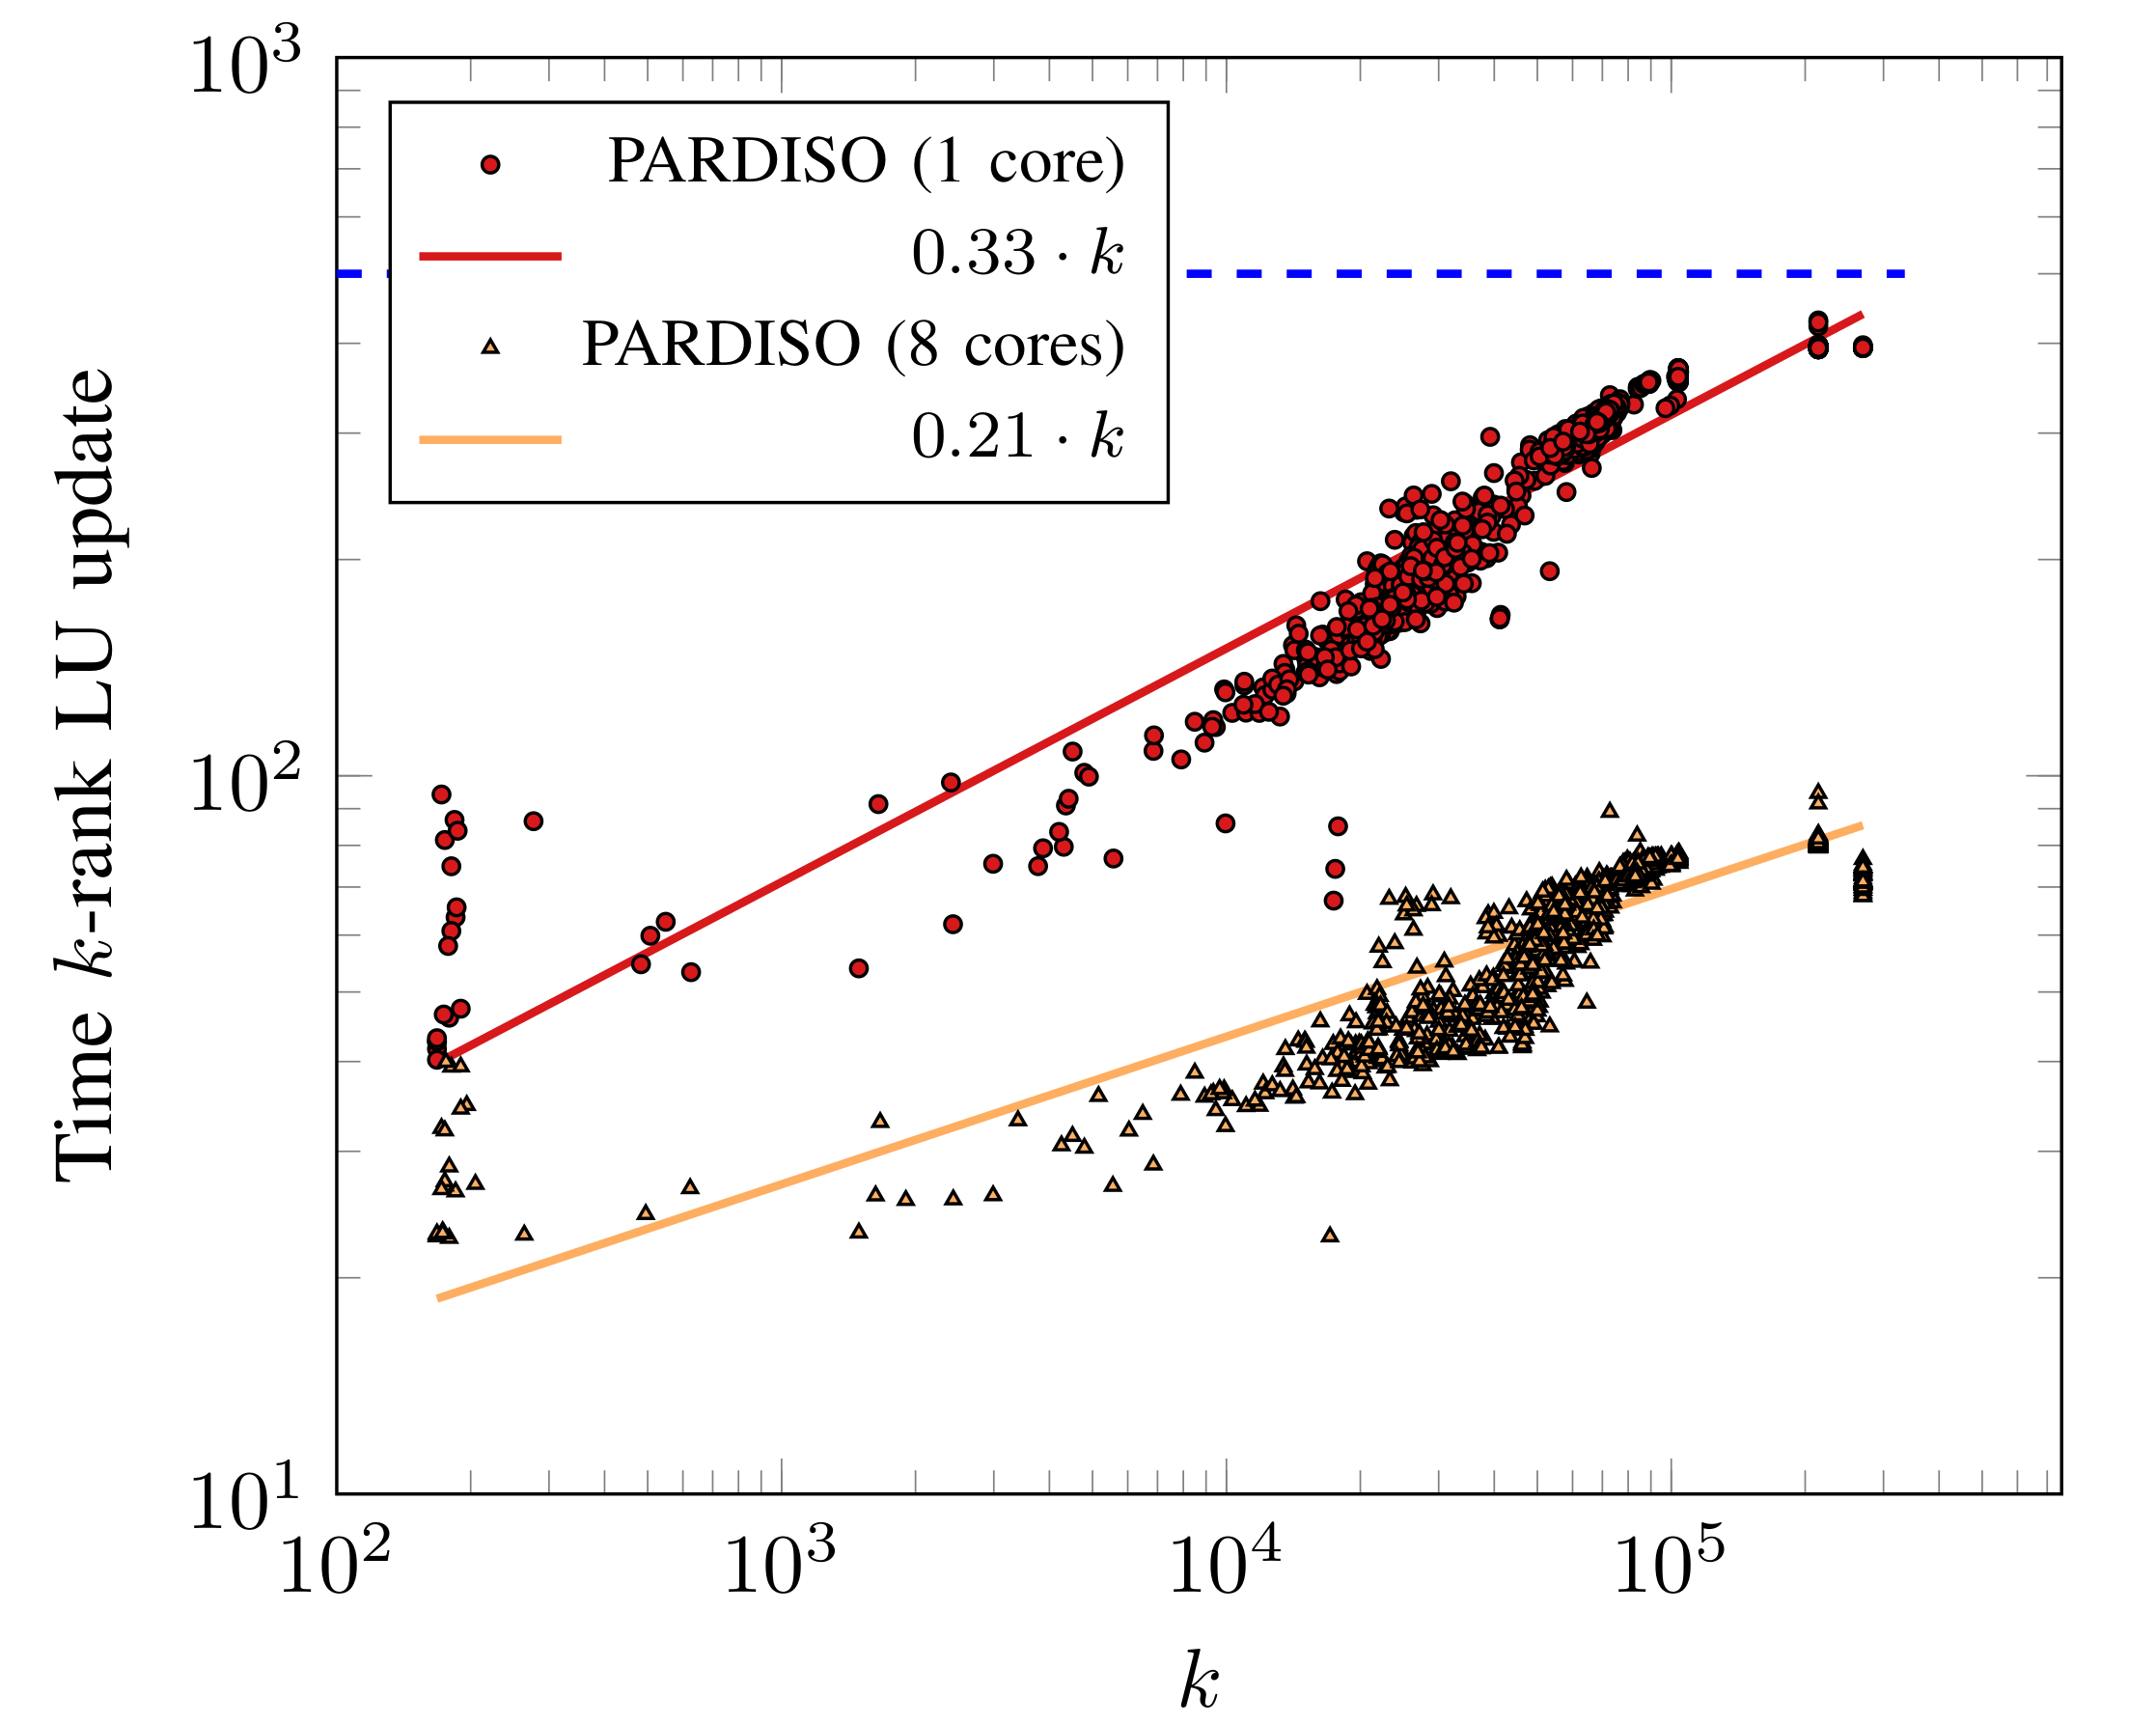
\includegraphics[width=0.5\textwidth]{figures/update} 
%
%     \caption{Regression analysis on the rank-$k$ update $LU$
%       factorization in PARDISO. }
%     \label{fig:incrementalLU}
%\end{wrapfigure}
%Newton iteration to the next, and from one timepoint to the next. As
%the matrix depends on the time-step, some simulators hold the
%time-steps constant as much as feasible to allow increased reuse of
%matrix factorizations. The nonzero entries of a matrix change only
%when the transistors and other nonlinear devices change their
%operation point. In most circuits, very few devices change state from
%one iteration to the next and from one time-step to the
%next. Nonzeros contributed by entirely linear components do not change
%value during the simulation. This makes incremental LU
%factorization a very useful feature of any matrix solver used in
%circuit simulation.  As of April 2019 the version PARDISO 6.2
% has a very efficient exploitation of
%incremental LU factorization, both serial and parallel.   In
%Figure~\ref{fig:incrementalLU} we show that PARDISO scales linearly
%with number of updated columns, and also scales well with number of
%cores. Here, the series of matrices were obtained from a full
%simulation of a post-layout circuit that includes all interconnects, 
%power- and ground-networks). The factorization time is plotted against the number of
%columns that changed compared to the previous factorization.
%The scatter plot shows the number of
%rank-$k$ update and the corresponding factorization time in
%       milliseconds. The regression analysis clearly demonstrates a
%       linear trend both for the single and the multiple core
%       versions. The dashed line shows the time for the full
%       factorization.
%
%Another recent useful feature in PARDISO is parallel selective inverse matrix computation as
%demonstrated in Table~\ref{table:bench_matrices}.
%In circuit simulation, the diagonal of the inverse matrix is the
%driving point impedance. It is often required to flag nodes in the
%circuit with very high driving point impedance. Such nodes would
%indicate failed interfaces between different subcircuits, leading to
%undefined state and high current leakage and power dissipation. A
%naive approach to this is to solve for the driving point impedance,
%the diagonal of the inverse matrix, by $N$ triangular solves. This is
%sometimes unacceptably expensive even with exploiting the sparsity of the
%right hand side, and minimizing the number of entries needed in the diagonal of the inverse.
%To bypass this complexity, heuristics to compute the impedance of 
%connected components are used. But this is error prone with many
%false positives and also false negatives. In the circuit Freescale, PARDISO, e.g., finished the
%required impedance calculations in 11.9 seconds compared to the
%traditional computation that consumed 162.9 hours.
%
%
%\begin{table}[t]
%	\centering
%%	\footnotesize
%	\caption{Details of the benchmark matrices. 'N' is the number of matrix rows and 'nnz' is the number of nonzeros. The table
%                shows the fill-in factor related to the numbers of nonzeros in $\frac{L+U}{A}$, the time for computing all diagonal elements 
%                of the inverse $A^{-1}$ using $N$ multiple forward/backward substitution in hours, and  using the selected inverse method in 
%		PARDISO for computing all diagonal elements of  the inverse $A^{-1}$ in seconds.}
%	\begin{center}
%\begin{tabular}{|l|r|r|c|r|r|}\hline
%\multicolumn{1}{|c|}{Matrix}  & 
%\multicolumn{1}{c|}{N}       &
%\multicolumn{1}{c|}{nnz$(A)$}&
%\multicolumn{1}{c|}{nnz$(\frac{L+U}{A})$} &  
%\multicolumn{1}{c|}{$A^{-1}$} & 
%\multicolumn{1}{c|}{Selected $A^{-1}$}  \\\hline
%{circuit5M\_DC}	&  3,523,317   & 19,194,193	&  2.87  &  82.3 h.    &  1.3 s.\\
%{circuit5M}	&  5,558,326   & 59,524,291	&  1.04  & 371.1 h.    &  2.1 s. \\
%{Freescale}	&  3,428,755   & 18,920,347	&  2.94  & 89.8 h.     &  1.0 s. \\
%{Freescale2}	&  2,999,349   & 23,042,677	&  2.92  & 8.5  h.      &  1.2 s. \\
%{FullChip}	&  2,987,012   & 26,621,990	&  7.41  & 162.9 h.      &  11.9 s. \\
%{memchip}	&  2,707,524   & 14,810,202	&  4.40  & 62.5 h.     & 0.9 s. \\\hline
%%#TABLE_DATA#
%
%\end{tabular}
% \label{table:bench_matrices}
%	\end{center}
%\end{table}
%
%
%
%The productivity gap in simulation continues to grow, and challenges
%remain.  Signoff simulations demand 10X speedup in sparse matrix
%factorization. Simply using more cores does not help unless the matrices
%are very large and complex. For a majority of simulations, scaling beyond
%8 cores is difficult. As a result, some of these
%simulations can take a few months to complete, making them essentially
%impossible. Some of the problems in parallelizing sparse matrix
%operations for circuit simulation are fundamental. Others may be related
%to implementation.  Research on sparse matrix factorization for circuit simulation
%continues to draw attention, especially in the area of acceleration
%with Intel's many integrated core (MIC) architecture \cite{Booth2017}
%and GPUs \cite{Chen2015, Nakhla2018}. Other techniques for
%acceleration include improved preconditioners for iterative solvers
%\cite{Feng2015}. We are presently addressing the need for runtime selection of
%optimal strategies for factorization, and also GPU acceleration. Given
%that circuits present a wide spectrum of matrices, no matter how we
%categorize them, it is possible to obtain a solver that is 2-10$\times$
%better on a given problem.  Improvements in parallel sparse matrix
%factorization targeted at circuit simulation is more necessary today
%than ever and will continue to drive applicability of traditional
%SPICE simulation methods.  Availability of sparse matrix packages such
%as PARDISO that completely satisfy the needs of various circuit
%simulation methods is necessary for continued performance gains.

\section[Sparse Linear Factorization Solvers]{High-Performance Computing Mathematical Libraries -- Sparse Linear Factorization Solvers}
High-performance  computing mathematical libraries have been a very important part of scientific and engineering computing for years, and their importance continues to grow as microprocessor architectures become more complex and software libraries become better designed to integrate easily within applications. Despite the fact that there are various science and engineering applications, the underlying algorithms typically have remarkable similarities, especially those algorithms that are most challenging to implement well in parallel. It is not too strong a statement to say that these software libraries are essential to the broad success of scalable high-performance computing in computational sciences (\cite{kothe-2007,pitac-2005,bader-2007}).

The recent trends in hardware development have added additional questions to this scenario, because today's codes are not guaranteed to exploit the performance of next-generation hardware to a satisfying degree. The so-called memory wall, i.e., the increasing performance gap between memory access and processor speed, will force scientific computing software to deal with the efficient use of complex multiple memory hierarchies. In addition, many-core architectures with hundreds of cores using a decreased processor clock rate will add additional algorithmic and software challenges to scientific computing. Autotuning tools, libraries, and software tools based on dwarfs \todol{[15]} will be designed that will help researcher and application developer to improve the performance of a given application.

The innermost computational kernels of many large-scale scientific applications and industrial numerical simulations are often either a large sparse matrix problem or a nonlinear optimization method which again can be reduced to a large sparse matrix problem. Sparse direct linear solvers are a core part of many problems in computational science and typically consume a significant portion of the overall computational time required by the simulations. While on one hand modern computer architectures provide larger memory resources and faster multicore processors, on the other hand the need for solving large scale application problems often compensates for these developments. The request for fast and memory efficient -- and robust -- solvers has been important for many years and remains an open field for further developments.

As mentioned before the use of graph pivoting techniques as an alternative approach to traditional pivoting methods emerged two decades ago (\cite{schenk-2004}). These graph-based methods
typically build a bipartite graph of a symmetric indefinite matrix A and, by traversing vertices and edges in the graph, these approaches compute a maximum weighted matching that
in turn defines a permutation of the rows and/or columns in A. The important advantage of
all these methods is that they allow -- in a parallel environment -- the precomputation of the
underlying elimination process, thus making the Gaussian elimination process much more
scalable. Almost all modern parallel sparse direct solver tools (see Table \ref{tab:solvers})
are now using these kinds of graph-pivoting techniques, since they are the key for high sequential and parallel efficiency.

For sparse direct algorithms there exist a wide range of possible methods, such as multifrontal, left- or right-looking supernodal methods, or a combination of these methods (\cite{davis:2006:dms}). As a result, different high-level implementations are available, such as SuperLU (\cite{superlu_dist}), Mumps \todol{[4]}, PARDISO (\cite{schenk-2004,schenk-2006}) and WSMP (\cite{gup02}). The communication patterns of all these different packages and methods are -- more or less -- very similar. All of them are using supernodal blocking strategies and this data structure will be used for performance modeling in the next chapters.

The Table \ref{tab:solvers} lists a few available software packages for the direct solution of sparse linear algebra problems. The interest is in software for high-performance computers for solving problems in numerical linear algebra, especially sparse direct systems.

\begin{table}[]
   \centering
   \begin{adjustbox}{angle=90}
\begin{tabular}{|l|l|c|c|c|c|c|c|c|c|c|c|}
\hline
   \multicolumn{1}{|c|}{SPARSE DIRECT SOLVERS} & \multicolumn{1}{c|}{License}  & \multicolumn{2}{c|}{Type} & Language  & \multicolumn{3}{c|}{Mode} & \multicolumn{3}{c|}{Sparse Direct} & Last release date \\ \hline
                      &          & Real       & Complex      &           & Shared  & Accel.  & Dist  & SPD         & SI       & Gen       &                   \\ \hline
DSCPACK               & PD       & X          &              & C         & X       &         & M     & X           &          &           & 2015-05-23        \\ \hline
KKTDirect             & PD       & X          &              & C/C++     & X       &         &       & LDLT        &          &           & 2010-04-21        \\ \hline
MUMPS                 & CeCILL-C & X          & X            & F77/F95   & X       &         & M     & X           & X        & X         & 2021-04-16        \\ \hline
Myramath              & GPL      & X          & X            & C++       & X       &         &       & X           & X        &           & 2020-05-20        \\ \hline
PaStiX                & LGPL     & X          & X            & F95/C/C++ & X       & C       & M     & X           & X        & X         & 2021-04-08        \\ \hline
PSPASES               & Own      & X          &              & F77/F95/C &         &         & M     & X           &          &           & 1999-05-09        \\ \hline
qr\_mumps             & LGPL     & X          & X            & F77/F95/C & X       & C       &       & X           &          & X         & 2021-04-2021      \\ \hline
Quern                 & PD       & X          &              & C/C++     & X       &         &       &             &          & X         & 2009-02-04        \\ \hline
SPARSE                & Own      & X          & X            & C         & X       &         &       & X           &          & X         & 1988-04-01        \\ \hline
SPOOLES               & PD       & X          & X            & C         & X       &         & M     &             &          & X         & 1999-04-08        \\ \hline
SPRAL                 & New BSD  & X          & X            & F77/F95/C & X       & C       &       & X           & X        &           & 2016-09-23        \\ \hline
SuiteSparse           & LGPL/GPL & X          & X            & C         & X       & C       &       & X           &          & X         & 2018-07-05        \\ \hline
SuperLU               & BSD      & X          & X            & F77/F95/C & X       & C       & M     &             &          & X         & 2020-10-17        \\ \hline
TAUCS                 & Own      & X          & X            & C         & X       &         &       & X           &          & X         & 2003-09-04        \\ \hline
Trilinos/Amesos       & LGPL     & X          &              & C/C++     & X       &         & M     & X           &          & X         & 2017-09-07        \\ \hline
Trilinos/Amesos2      & BSD      & X          & X            & C++       & X       &         & M     & X           &          & X         & 2017-09-07        \\ \hline
Y12M                  & ?        & X          &              & F77/F95   & X       &         &       & X           &          & X         & ?                 \\ \hline
\end{tabular}
   \end{adjustbox}
   \caption{List of some sparse direct solvers from \url{https://docs.google.com/spreadsheets/d/11ESR3uucNvVKEoIcalP9gR7ApaOElLwmE5sAS-VRMOM/edit\#gid=90156307}}
   \label{tab:solvers}
\end{table}

%https://docs.google.com/spreadsheets/d/11ESR3uucNvVKEoIcalP9gR7ApaOElLwmE5sAS-VRMOM/edit#gid=90156307

\chapter{Performance Modeling of Sparse Factorization Solvers}

%{\color{blue} juraj: introduction to performance modelling: know the max performance limit before doing further optimizations, what is the hw utilization of the code?}

Performance engineering plays an important role in development of scientific software. In order to achieve optimal performance, one needs to analyze the code and computer architecture to identify bottlenecks and possibilities for optimization. This helps us spend our effort only where there is a potential for improvement.
%It is also useful to have realistic expectations about performance given code can achieve.
While simple code can be often analyzed using intuition and guessing, this is not possible for nontrivial codes. Performance models are helping us to analyze a code by guiding our attention on important features and neglecting unnecessary details.
%
%In this chapter we analyze forward and backward substitution code used in direct methods for solving sparse linear systems. Due to the fact that part of the algorithm is executed sequentially and part in parallel, the performance predictions are challenging. With our extension to the roofline model we are able to model such code. The predictions are then compared to measurements for a representative set of sparse matrices.
%
%Last, the Execution-Cache-Memory (ECM) model is studied as a theoretical base for use for modeling of forward and backward substitution \todol{in the next chapter}.
%Unlike the roofline model, ECM takes into account deep knowledge of the computer architecture, in particular in-core execution and cache hierarchy, which might allow it more accurate predictions.
%
This chapter reviews two performance models we will later use for modeling forward and backward substitution code used in sparse factorization solvers.

The chapter is organized as follows. In Section \ref{sec:arch} computer architecture is briefly introduced. Next, Section \ref{sec:likwid} reviews command line tools called LIKWID. These tools are useful for various performance engineering tasks, e.g. determining the hardware and its specification, micro-benchmarking and profiling. After that, two established performance models are reviewed: Berkeley Roofline model in Section \ref{sec:roofline} and Erlangen Execution-cache-memory model in Section \ref{sec:ecm}. Finally in Section \ref{sec:ecm-application} Execution-cache-memory model is used to analyze performance of two simple computational kernels. Models of these two kernels will be later used as a base for modeling sparse triangular solve.

%\section{Code parameters}
%
%\subsection*{Work}
%
%With $W$ we denote work. It is the number of operations executed by a program or algorithm. It could refer to any type of operation, but here we always measure work in floating point operations (FLOPs) in double precision.
%We don't count instructions because one instruction can perform more than one floating point operation.
%
%In kernels like dot product, there is often multiplication followed by addition. To make these computations more efficient, many modern CPU architectures compute operations similar to $a=a+b*c$ in one instruction. This type of instructions is called fused multiply-add (FMA).
%Other widely used computation is applying the same operation on many operands, vector addition $A[:]=B[:]+C[:]$. This is in hardware implemented using so called vector instructions. Advanced Vector Extensions (AVX) operates on registers of size 256\,b, which can store 4 operands in double precision or 8 in single precision. One AVX instruction performs 4 FLOPs. And AVX2 adds support of vectorized FMA operations, so 8 FLOPs are performed in a single instruction.
%
%\subsection*{Performance}
%
%Performance refers to number of operations per unit of time.
%If program finishes performs $W$ operations and finishes the computations in time $T$, then it achieves performance $P = W/T$.
%
%\subsection*{Memory traffic}
%
%Before processor can perform computations, data has to be loaded to registers. The data has to travel form memory to the L3 cache, then to L2 and L1 and finally to the registers. The registers and cache have very limited size, so after the computations when the data are not needed anymore, it has to travel through the hierarchy back to memory.
%
%We denote the data transferred from memory to L3 cache $Q_r$ (read) and the data transferred from L3 cache to memory $Q_w$ (write), all measured in bytes. The memory traffic is $Q = Q_r + Q_w$.
%We could also examine traffic between different cache levels, but for the memory traffic we are interested only in the data transferred between memory and the L3 cache.
%
%\subsection*{Operational intensity and code balance}
%
%The operational intensity is a ratio between work and memory traffic $I = W / Q$, number of floating point operations for 1\,B or memory transfer.
%Similar to operational intensity is arithmetic intensity, but it is defined as \todol{todo}.
%
%Sometimes it is more convenient using code balance instead of operational intensity. This is defined as $B_c = I^{-1} = Q / W$, number of bytes per one floating point operation.
%
%\section{Machine parameters}
%
%\subsection*{Peak performance}
%
%Peak performance is theoretical maximum the processor is designed to compute. To achieve the peak performance, the processor must utilize all cores and in every cycle it executes the instructions that compute the most operations. Typically these are the AVX (4 FLOPs/cycle) or AVX2 instructions (8 FLOPs/cycle).
%As and example let's look at an Intel Xeon E5-2695 v3. This is a 14 core CPU with Haswell architecture and frequency 2.3\.GHz. The Haswell architecture supports AVX2 and can execute two instructions per cycle.
%So the peak performance is $P_{peak} = 2.3 * 14 * 8 * 2 = 515.2\,\textrm{GFLOPs/s}$.
%Evaluation of the peak performance of modern CPUs is not as easy as it seems. It depends on an instruction set and number and type of units in a core. Nice analysis of different Intel architectures can be found in \cite{dolbeau-2018}.
%
%However, the peak performance is a theoretical maximum that most real world applications are not able to achieve.
%For example if compiler cannot vectorize the code, the performance drops by factor of four. And if a kernel uses only addition or only multiplication, for example sum of elements in a vector, then the performance drops to a half.
%Instead of peak performance we use attainable performance, denoted as $P_{max}$. This allows more realistic expectations based on knowledge of the code and instructions set used by the compiler.
%
%\subsection*{Memory bandwidth}
%
%Memory bandwidth $b_s$ is a rate at which data can be read and stored into memory.
%The bandwidth found in a datasheet does not have to be reachable by the app, similar to the peak performance.
%The memory bandwidth depends on access pattern, number of threads, if NUMA is used and Cluster-on-Die\footnote{Cluster-on-Die (CoD) solves a problem with saturation of memory bandwidth on server CPUs from Intel. These CPUs have many cores (14 or more), but only few can are able to saturate the memory bandwidth. When CoD is enabled, the cores, memory and L3 cache are split to two NUMA domains and second memory controller is used. This reduces the number of cores using the same memory controller and doubles the memory bandwidth.} enabled.
%More realistic bandwidth can be obtained using micro-benchmark, ideally with similar memory access pattern as the application.
%
%\subsection*{Machine balance}
%
%Machine balance $B_m = b_s / P_{max}$ is a ratio of memory bandwidth and attainable performance.
%If $B_c < B_m$ then the code’s performance is limited by the max performance, it is compute bound. Optimizing memory access of such code does not improve performance. One should focus on optimizing computations, for example using vector instructions as much as possible.
%If $B_c > B_m$ then the code’s performance is limited by the memory bandwidth, hence it is memory bound. Here performance can be improved by optimizing memory access pattern, for example by reusing data loaded to cache us much as possible, so they don't have to be loaded from memory.

\section[Introduction --- Memory Hierarchies, Autotuning, and Solvers]{Introduction --- Exploiting the Memory Hierarchies, Autotuning Research, and Sparse Factorization Solvers}
\label{sec:modeling-intro}

Modern microprocessors are highly sensitive to the spatial and temporal locality of data. Regardless of the programming model, performance of future parallel applications will crucially depend on the quality of the generated code which is traditionally the responsibility of the compiler. The compiler selects which optimization to perform in terms of, e.g., loop-unrolling, out-of-order instruction capabilities, or register scheduling. Choosing parameters for these optimizations, and selecting among alternative implementations, is the key to efficient use of the underlying hardware. The resulting space of optimization alternative is large.

Autotuner projects such as, e.g. ATLAS~\footnote{Automatically Tuned Linear Algebra Software} (\cite{atlas-hp,whaley04,WN147}), FLAME~\footnote{Formal Linear Algebra Methods Environment} (\cite{Flame:2005}), and OSKI~\footnote{Optimized Sparse Kernel Interface} (\cite{Demmel2005:selftune:linalg,Vuduc2003:thesis,Lee2004:spmv:symm}),
gained popularity as a very effective approach for producing high-quality portable scientific code. In these projects, the set of library kernels is automatically optimized by generating many variants of a given kernel and by running that kernel in a target platform. The search process may take hours to complete on the platform. However, it needs to be performed only once when the library is installed on the platform. The resulting codes might be
several times faster than naive implementations.

As an example, reordering the vertices and elements in a mesh can have a significant impact on performance. Graph and hypergraph techniques have been used in this area to automatically generate highly efficient, platform-adapted implementations of {\sl sparse matrix kernels}. These kernels are frequently computational bottlenecks in diverse applications in computational science and engineering applications. However, the task of extracting near-peak performance on modern cache-based superscalar machines has proven to be extremely difficult. Many sparse matrices from applications have a natural block structure that can be exploited by storing columns as a collection of blocks and thus accelerating the performance of sparse matrix kernels significantly. It is shown in recent projects such as \cite{BEBOP2016,Vuduc2003:thesis} that it is possible to build an automatic tuning system to generate implementations whose performances exceed that of the best hand-tuned code. The algorithmic methods behind these research projects are based on reordering methods on the discrete graph structure in order to maximize the block structure and, thus, obtaining high performance by maximizing spatial and temporal locality.

\todop{update references to newer}

\section{Computer architecture}
\label{sec:arch}

%\todop{
%+ cores
%+ ports (image)
%+ out of order !!!!!
%+ instrucitons (pipeline, Haswell, ...)
%+ AVX
%+ FMA
%+ NUMA
%+ CoD
%+ Peak performance (all together)
%+ Memory bandwidth
%}

Modern processors utilize numerous techniques that aim to improve performance --- the number of computations done per unit of time. In the past, the performance used to be increased only by increasing the CPU clock frequency. However, increasing the frequency results in higher power consumption and, consequently, the CPU needs a larger heat sink in order to prevent it from overheating. As a result, the clock frequency of recent CPUs is about 2.0--3.5\,GHz and does not increase anymore.
Since the trend of doing computations faster due to increasing frequency is over, the effort of CPU manufacturers focuses on performing computations at the same time in parallel.
This leads to adding more computational units to modern processors. These units, called cores, perform instructions independently, thus the overall performance is effectively increased. This scheme works well when every core works on different data, but when an access to shared data is required the cores need to be synchronized in order to prevent data conflicts and inconsistent results. The synchronization, however, requires serialization of computation and prevention parallel computations, thus reducing the overall performance.

Another possibility for parallel computations is implementing instructions that perform more than one operation applied on vectors of data instead of single elements. Such instructions are called SIMD (Single Instruction Multiple Data), examples of which are SSE (Streaming SIMD Extensions) that operates on 128\,b registers containing two floating point numbers in double precision or four numbers in single precision, or newer AVX (Advanced Vector Extensions) with registers twice as big, computing four operations in double precision in a single instruction.

Another CPU optimization focuses on computational pattern, where there is multiplication followed by addition. An example of such an operation can be found in many compute kernels in various scientific applications. In order to make these computations more efficient, many modern CPU architectures compute operations similar to $a=a+b*c$ in one instruction. This type of instruction is called fused multiply-add (FMA).
The new version of an AVX extension, called AVX2, adds support for vectorized FMA operations, effectively performing 8 operations in a single instruction using double precision (16 operations in single precision).

\begin{figure}[t]
  \centering
  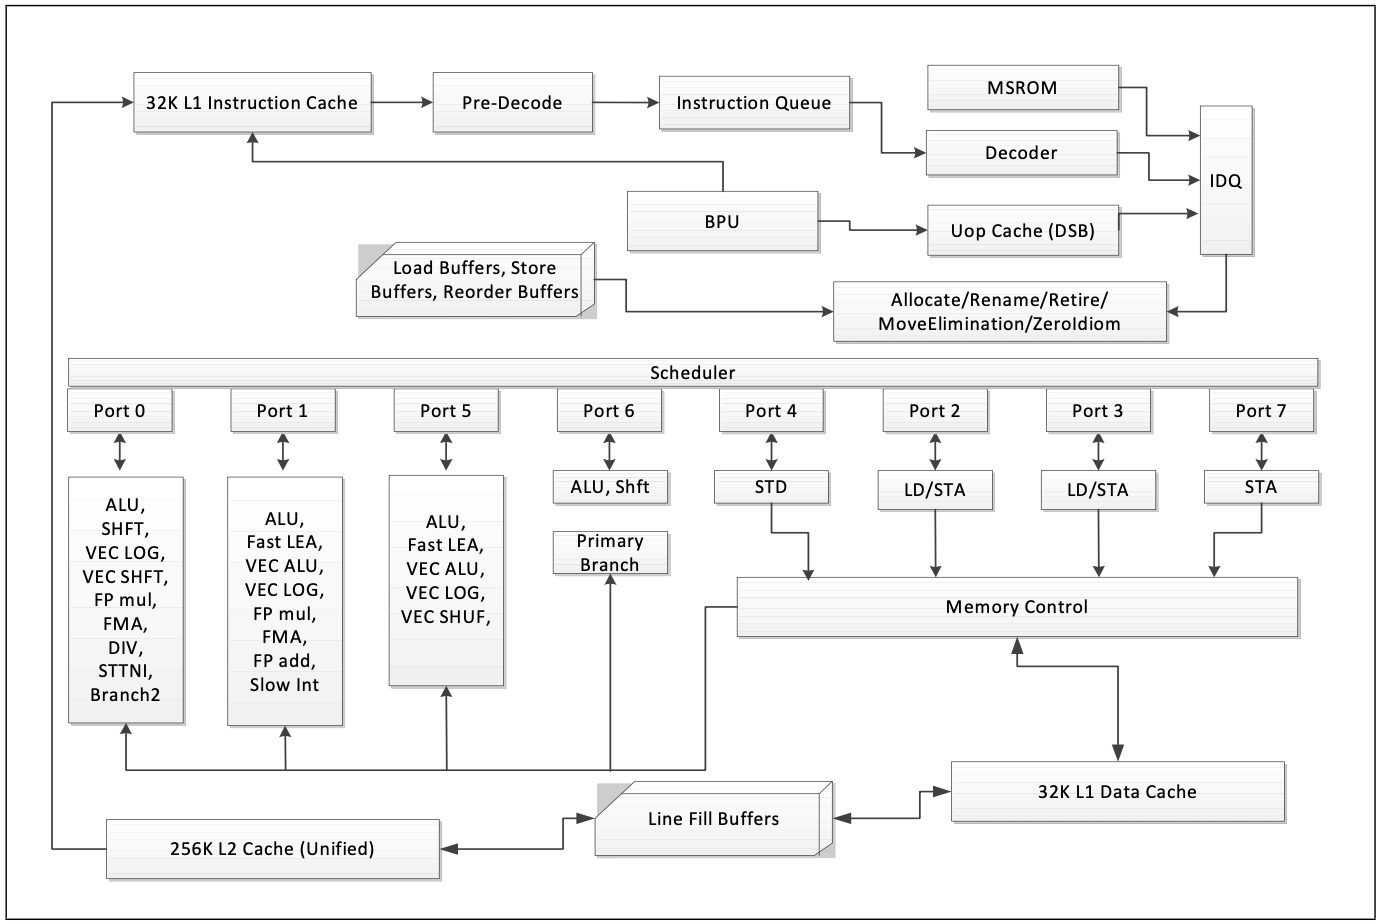
\includegraphics[width=\textwidth]{images/haswell_microarchitecture.png}
  \caption{CPU core pipeline of Haswell microarchitecture. From \cite{intel-orm-2016}.}
  \label{fig:hsw-microarch}
\end{figure}

The parallelism can be exploited not only on the level of multiple cores, but also on the instruction-level within a single processor, an example of which is instruction pipelining. Pipelining attempts to divide incoming instructions into a series of sequential steps, allowing the processor to dispatch a new instruction every cycle, instead of performing a whole instruction which takes several cycles. Additionally, in order to maximize instruction throughput, the instructions are executed out of order, if there are available processing units.
A CPU core of Intel Haswell microarchitecture is shown in Figure \ref{fig:hsw-microarch}, consisting of eight dispatch ports in total, four of which have units for computational operations and four for memory operations. The scheduler can dispatch up to eight micro-ops every cycle, one on each port.

Another level of complexity is introduced when considering data movements. The CPU performs all operations on data stored in registers, the fast but small memory inside the CPU. Before the computations start, data have to first be loaded from memory to registers and when the computations are done, they have to be stored back to memory. The memory is very slow compared to the registers, which introduces a significant bottleneck hampering the performance of a computation. To make the memory access more efficient there are multiple levels of memory between the CPU and main memory, each with different size and access speed, referred to as cache. Usually the cache has three levels, called L1, L2, and L3. L1 is closest to the CPU and has the smallest size (few kB), while L3 is closest to the memory and has the largest size (few MB). Any data transferred between the memory and registers have to go through all cache levels. 
In some cases data are often reused in the computation, thus they can stay in the cache, avoiding communication with the slow memory.

In order to improve performance and the ability of the system to be expanded, e.g., in the case of servers often having more than one processor, every processor has its own memory and memory controller. This memory layout is called NUMA (Non-Uniform Memory Access). The benefit of such an architecture is that it increases memory bandwidth, the rate at which data can be read and stored into memory, which prevents a~bottleneck introduced by all the cores accessing the memory and saturating the available bandwidth, resulting in idle cores waiting for data instead of doing useful computation. On the other hand, introducing multiple memory domains creates problems when one processor needs to access data in memory belonging to another processor. This situation is possible but not very efficient, as it increases the load at a single memory controller and, additionally, the data have to be transferred through a link between processors, which can become a bottleneck. The programmer works with a virtual memory spanning all memory domains, so he does not see this underlying complexity, but he should keep this in mind in order to write efficient code. For example, an operating system places memory pages to the physical memory of the processor that writes to the page for the first time, so called first touch. If a single thread initializes all the data that are then accessed in parallel, it might allocate the data in a suboptimal way. If the initialization is performed in parallel, significantly better memory utilization can be achieved.

\begin{table*}[t]
%\parbox{.7\linewidth}{
  \footnotesize
 \centering
%\resizebox{\textwidth}{!}{%
 \begin{tabular}{p{1.9cm}llrrrrrrrrr}
    \hline
    name      & &  & IVB         & HSW-D      & HSW-S           & BDW           & SKX         & KNL           & ZEN-D        &  ZEN-S         \\
    \hline
    \multirow{3}{\linewidth}{processor name} & &  & Intel& Intel & Intel & Intel & Intel & Intel & AMD &  AMD \\
      & &  & Xeon  & Xeon & Xeon      & Xeon    & Xeon  & Xeon    &
~~Ryzen 7   &  ~~EPYC      \\
              & &  &\scriptsize  E5-2660 v2 &\scriptsize  E3-1240 v3
&\scriptsize  E5-2695 v3      &\scriptsize  E5-2630 v4    &\scriptsize  Gold
6148   &\scriptsize  Phi 7210      &\scriptsize  1700X      &\scriptsize
745           \\
%     processor & &  & Intel Xeon  & Intel Xeon & Intel Xeon      & Intel Xeon    & Intel Xeon  & Intel Xeon    & AMD Ryzen    &  AMD EPYC      \\
%     name      & &  &  E5-2660 v2 & E3-1240 v3 & E5-2695 v3      & E5-2630 v4    & Gold 6148   & Phi 7210      & 7 1700X      &  745           \\
    \hline
    micro     & &  & Ivy Bridge  & Haswell    & Haswell         & Broadwell
& Skylake     & ~Knigths       & Zen          &  Zen           \\
    arch.     & &  &             &            &                 &               &             & Landing       & \\
    \hline
    freq    & [GHz] & & 2.2      & 3.4        & 2.3             & 2.2           & 2.4         & $\approx$ 1.3 & 3.4          &  2.3           \\
    cores   &       & & 10       & 4          & 2 $\times$ 7    & 10            & 20          & 64            &   8          &  24            \\
    ISA     &       & & AVX      & AVX2       & AVX2            & AVX2          & AVX-512     & AVX-512       & AVX2         &  AVX2          \\
%    sockets &       & 2        & 1          & 2               & 2             & 2           & 1             & 1            &  & 1 \\
%    \mltwo{NUMA LDs}& 2        & 1          & 2 $\times$ 2    & 2 $\times$ 2  & 2           & 1             & 1            &  & 1 \\
    \mltwo{NUMA LDs} & & 1       & 1          & 2               & 1             & 1           & 1             & 1            & 4              \\
    \hline
    L1 & [KiB]     &  &  32      & 32         & 32              & 32            & 32          & 32            & 32           &  32            \\
    L2 & [KiB]     &  &  256     & 256        & 256             & 256           & 1024        & 1024          & 512          &  512           \\
    L3 & [MiB]     &  &  25      & 8          & 2 $\times$ 17.5 & 25            & 28          & -             & 2 $\times$ 8 &  8 $\times$ 8 \\
    \hline
%    copy bw. & [GB/s] & 41.2   & 26.6            & 22.6       & 31.3 & ?? &  75.9 & 30.2 & 212 \\ % complete socket/cod
%    read bw. & [GB/s] & 44.3   & 30.9            & 23.6       & 33.7 & ?? &  74.2 & 32.5 & 231 \\ % complete socket/cod
    \mlfour{scalar read bw.}   &     &          &  \\
    ~1 core  & [GB/s]  &&  9.5 & 16.6 & 12.1 & 11.5 &  14.5 &  8.5 & 19.3 & 19.3  \\
    ~NUMA LD & [GB/s]  && 44.4 & 22.7 & 31.2 & 56.3 & 108.0 & 75.2 & 33.7 & 37.6  \\
    \hline
    \mlfour{scalar ADD+MUL/FMA} &&& \\
    ~1 core  & [F/cy] &&  2 &  4 &  4 &  4 &  4 &   4 &  4 &  4 \\
    ~NUMA LD & [F/cy] && 20 & 16 & 28 & 40 & 80 & 256 & 32 & 24 \\
    \hline
    \mlfour{scalar machine balance $B_m$} &  &         & \\
    ~1 core  & [B/F] && 2.2 & 1.2 & 1.3 & 1.3 & 1.5 & 1.6 & 1.4 & 2.1 \\
    ~NUMA LD & [B/F] && 1.0 & 0.4 & 0.5 & 0.6 & 0.6 & 0.2 & 0.3 & 0.7 \\
    \hline
\\[0.01em]
  \end{tabular}
  \caption{Details of Evaluated Hardware Systems.
% ISA Lists the Latest Extension Supported by the Processor.
% Read Memory Bandwidth, Floating Point Instructions per Cycle (ADD+MULL and
% FMA Instructions), and Machine Balance is Reported for Scalar Execution.
KNL's Bandwidth Numbers are for DDR Memory.}
% ECM: 2 cy L1/L2 bei HSW/BDW entgegen der Doku
% STREAM:
% read = summation
% KNL: no-nt, prefetch not explicitly disabled
% ZEN: no-nt, AVX2, only even cores
% HSW2: no-nt, avx2
% HSW: no-nt, avx2
% IVB: no-nt,
  \label{tab:hw}
%} % from https://tex.stackexchange.com/a/27105
%}
\end{table*}

Modern server processors contain a lot of cores (usually 14 or more) and with so many cores accessing the memory it is very easy to saturate the memory bandwidth. Intel solves this problem by splitting the memory and L3 cache between two NUMA domains and use second memory controller. This reduces the number of cores using the same memory controller and doubles the memory bandwidth. Intel calls this architecture Cluster-on-Die (CoD).
%Cluster-on-Die (CoD) solves a problem with saturation of memory bandwidth on server CPUs from Intel. These CPUs have many cores (14 or more), but only few can are able to saturate the memory bandwidth. When CoD is enabled, the cores, memory and L3 cache are split to two NUMA domains and second memory controller is used. This reduces the number of cores using the same memory controller and doubles the memory bandwidth.

Peak performance of a CPU is a theoretical maximum the processor can\linebreak achieve. It requires utilization of all cores running at the base frequency and every core achieving the highest possible floating point throughput.
Evaluation of the peak performance of modern CPUs is a very intricate process, requiring one to consider a multitude of factors. It depends on an instruction set and the number and type of units in a core. A detailed analysis of different Intel architectures can be found in \cite{dolbeau-2018}.
As an example we can analyze Intel Xeon E5-2695 v3. This is a 14 core CPU with Haswell architecture and base frequency 2.3\,GHz (detailed description is in Table \ref{tab:hw}). The Haswell architecture supports AVX2 instructions (8 FLOPs per instruction) and can execute two instructions per cycle (ports 1 and 5), resulting in a total of 16 FLOPs per cycle per core.
Consequently, the peak performance is $P_{peak} = 2.3 * 14 * 8 * 2 = 515.2\,\textrm{GFLOPs/s}$.

The theoretical memory bandwidth can be found in a datasheet, but the attainable bandwidth of a specific application depends on the access patters, number of threads used, whether NUMA is used, and other factors. Using the theoretical bandwidth is thus not precise for purposes of performance analysis.
A more realistic bandwidth can be obtained using microbenchmarks, ideally with similar memory access patterns as the application.
%\texttt{likwid-bench} from the LIKWID toolbox is a popular application for benchmarking different kernels.
In the following section we will review a performance tool called LIKWID which supports software developers, benchmarkers and application users to model and get the best performance on a given system. We will use this tool later for performance modeling for a sparse factorization solver.

\section{Performance modelling using the LIKWID Tools}
\label{sec:likwid}

LIKWID ("Like I Knew What I'm Doing") (\cite{likwid-2010-arxiv}) is set of command line tools to support optimization and performance engineering.
It consists of tools that display thread and cache topology, discover CPU and memory performance using benchmarks, alter CPU frequency and other settings, and allow performance evaluation of user applications.
Typical workflow using the LIKWID tools could be (i) use \texttt{likwid-topology} to find information about the hardware, (ii) gather various performance metrics using \texttt{likwid-bench} (memory bandwidth, performance using different instruction sets, etc.). Next, (iii) run an application specifying thread affinity using \texttt{likwid-pin} and (iv) evaluate performance a of user application using \texttt{likwid-perfctr} by collecing performance metrics either for the whole runtime or only for a specified code region.
A short description of the most useful tools follows.

\subsection*{likwid-topology}

Performance engineering requires  in-depth knowledge about node topology, like NUMA domains, cache hierarchy and sizes, CPU architecture, frequency, cores, and HW threads.
This information can be gathered using various command line tools, which might be time consuming, especially since some of them present long output where it is difficult to find required information. \texttt{likwid-topology} provides a holistic picture of node topology, collecting information from different available sources in the operating system and presenting a comprehensive and easy to understand overview of the node topology either in intuitive text form or an ASCII art style.

\subsection*{likwid-pin}

Thread affinity is crucial for performance of scientific applications. Knowing the topology (obtained, for example, by \texttt{likwid-topology}), one can pin threads to cores according to the application's requirements.
Pinning threads make performance measurements more consistent between runs and usually also improve performance bacause the threads are not assigned to cores randomly. This is very important when multiple NUMA domains are used to minimize the data traffic between NUMA domains.
%
\texttt{likwid-pin} can be used with all applications based on POSIX threads, which include most of OpenMP implementations. The pinning is achieved by overloading the \texttt{pthread\_create} call and pinning every thread upon creation.
Some OpenMP implementations create shepherd threads. These threads do not execute any user code and therefore should not be pinned. This is achieved by providing a mask or using one of the predefined masks for known implementations.

\subsection*{likwid-perfctr}

All modern CPUs provide hardware counters, registers that can be set to count various hardware events. The main purpose of these counters is to help manufacturers with development of the CPU, but they are also available to the user. The counters are accessed using model specific registers (MSR) and can be configured to count various events like fetching data, storing data, cache hits/misses, or calculations. As the counters are implemented in hardware, they come with no overhead. A downside of using the counters is that they measure events on a given core and cannot distinguish between processes. However, on systems with only one user this is usually not a problem.

\texttt{likwid-perfctr} is a command line tool that configures and reads the counters and is used as a wrapper for a user application.
It can be used in two modes: it can either measure the whole runtime of the application or only specific blocks of code called regions.
If the whole runtime is measured, no modification of the application is needed.
For measuring the regions, markers denoting the beginning and end of a region have to be inserted into the application code and have to be linked with the likwid library. The markers are library function calls that read values of the counters. 
Every marker has a name (user defined string) identifying the region. The string does not have to be unique, but all regions with the same name are summed up and are indistinguishable in the output. 
After the user application finishes, the data from counters are processed and a summary is presented. As reading the counters is a simple operation and all the processing is done after the user app finishes, there is very little overhead.

The measured events are specified as command line arguments to the wrapper application, so the measurement can be repeated several times measuring different events without recompiling the code.
The raw counts usually do not provide a lot of insight. However, \texttt{likwid-perfctr} can combine the raw counts to derive useful performance metrics like FLOPs/s or memory bandwidth.
%
Additionally, \texttt{likwid-perfctr} has also functionality of \texttt{likwid-pin}. This is very important because without pinning the threads could move between cores, making the measurements inaccurate.

\subsection*{likwid-bench}

Writing a benchmark is a very intricate process. The purpose of a benchmark is to measure some specific computation; however, the naive user code might not necessarily be the most efficient implementation. A compiler exploits a lot of optimizations, e.g., if results of some computations are not used, these computations are often dropped altogether. Alternatively, a compiler can replace the user code by more efficient implementation. In both cases, the benchmark would end up measuring something different from what was intended.
To be sure the benchmark measures the proper thing, the code most likely has to be written in assembly or at least the user should check the assembly generated by a compiler.

\texttt{likwid-bench} is a benchmark suite for prototyping low-level assembly kernels. 
It contains a set of various kernels, for example, dot product, daxpy, load, store, copy, and many others. It allows the user to define his own kernels. The kernels are defined as text files that are compiled during compilation of the suite. And the suite takes care of everything else: running the kernel on a problem of a given size, on a given number of threads, and presenting results to the user.

\section[Berkeley Roofline model]{Berkeley Roofline model - A Performance Model for Multicore Architectures}
\label{sec:roofline}

Programmers often do not need an understanding of every detail of CPU design. They should focus on general concepts rather than details of every available architecture. A tool that can provide a simplified model of the CPU hiding most of the architecture specific complexity is very valuable. Probably the most popular tool was popularized by \cite{williams-2009}. This tool is called the Roofline model.
It became very popular because it hides most of the CPU complexity and presents an intuitive and easy to use model that can guide performance engineering.

%\todop{
%abstraction, hides detais (ports, ...)
%easy to use
%two bottlenecks
%shows maximum performance given code can achieve, useful when compared with measurements, we can see how far the measured performance is from the theoretical maximum
%}

The model analyzes bottlenecks during execution on a given hardware.
A compute kernel reads data from memory, does some computations, and writes the results back to memory. Let's denote $W$ as the size of data read or written to memory in Bytes and $F$ the number of operations the kernel computes. Usually we are interested in floating point operations (FLOPs), additions and multiplications, but we could generalize this to any kind of operations.
Let's assume the machine has peak performance $P_{peak}$ measured in [FLOPs/s] and peak memory bandwidth $b_s$ measured in [B/s].
It is reasonable to expect the processor needs $F/P_{peak}$\,s to finish all computations and it needs $W/b_s$\,s for the memory transfer (reading and writing data). If we assume the computation and memory transfer can perfectly overlap, the total runtime is equal to the one that take longer:
\begin{equation}
    T = \max(F/P_{peak}, W/b_s).
\end{equation}

Working with runtime is not very useful because it depends on the size of the problem. Instead we usually compare performance $P=F/T$ [FLOPs/s].
Let's also define arithmetic intensity as the number of operations per one byte of memory transfer, $I=F/W$. Then we can write the expected performance as
\begin{equation}
   P = min(P_{peak}, I \cdot b_s). \label{eq:roofline}
\end{equation}

Sometimes it is easier working with code balance instead of arithmetic intensity. Let's define code balance as the number of transferred bytes per one operation, $B_c=W/F=I^{-1}$. Then we can write (\ref{eq:roofline}) as
\begin{equation}
   P = min(P_{peak}, b_s/B_c). \label{eq:roofline_balance}
\end{equation}

\begin{figure}[t]
   \centering
   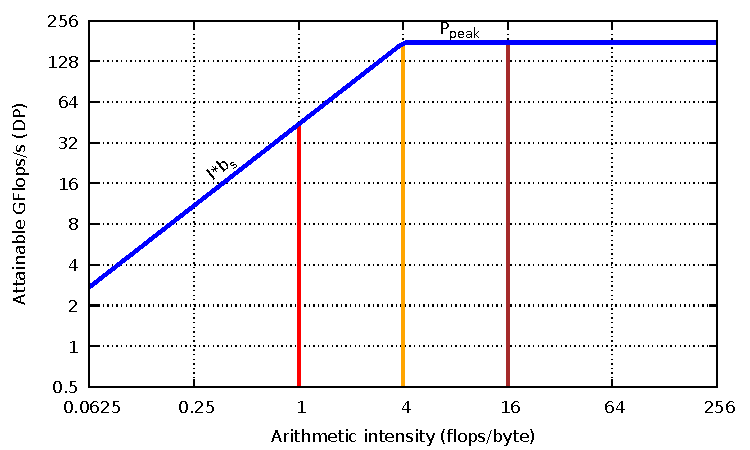
\includegraphics[width=0.7\textwidth,clip=true]{images/roofline/roofline_emmy_Xeon2660v2_naive.pdf}
   \caption{Roofline model of Intel Xeon E5-2660 v2 (blue) and three generic kernels (red, orange, and brown).}
  \label{fig:roofline_emmy_naive}
\end{figure}

We can see a graphical representation of (\ref{eq:roofline}) in Figure \ref{fig:roofline_emmy_naive} in a blue color. The shape of the graph looks like a roof, which gives the model its name.
The performance bound increases with increasing arithmetic intensity until it saturates at the peak performance. This happens where the two lines corresponding to the two bottlenecks intersect. The arithmetic intensity of this intersection equals $P_{peak}/b_s$ or machine balance $B_m=b_s/P_{peak}$. We call it machine balance and not code balance because it characterizes the machine.

In Figure \ref{fig:roofline_emmy_naive} we can also see three vertical lines. These lines represent three generic kernels with arithmetic intensity 1, 4, and 16. We can expect the performance of these kernels somewhere along the respective lines.
Note that the lines are below the roofline, since the roofline is the performance upper bound.
The red kernel (arithmetic intensity 1) is in the bandwidth limited region. The performance is increasing with increasing arithmetic intensity. Looking at the intersection of the red and blue line, we can expect a performance bound of approximately 44\,GFLOPs/s.
The brown kernel (arithmetic intensity 16) is in the compute bound region. With increasing arithmetic intensity the memory traffic decreases, but the performance does not increase.
And the orange kernel (arithmetic intensity $4 \approx B_m^{-1}$) is between these regions. Performance of this kernel depends on machine ability to overlap computation and memory communication (loads and stores).

%Machine balance $B_m = b_s / P_{max}$ is a ratio of memory bandwidth and attainable performance.
%If $B_c < B_m$ then the code’s performance is limited by the max performance, it is compute bound. Optimizing memory access of such code does not improve performance. One should focus on optimizing computations, for example using vector instructions as much as possible.
%If $B_c > B_m$ then the code’s performance is limited by the memory bandwidth, hence it is memory bound. Here performance can be improved by optimizing memory access pattern, for example by reusing data loaded to cache us much as possible, so they don't have to be loaded from memory.

%The point where the two lines intersect is at operational intensity $I = B_m^{-1}$. At this point the performance $P_{max}$ is achieved while reading and writing to memory as much as possible, $b_s$\,B/s.
%Performance of any kernel on the right side of this point ($B_c < B_m$ or $I > B_m^{-1}$) is limited by $P_{max}$. We call such kernel compute bound.
%Performance of any kernel on the left side of this point ($B_c > B_m$ or $I < B_m^{-1}$) is limited by $b_s$. We call such kernel memory bound.

\subsection{Roofline Ceilings}

For realistic applications the measured performance of a kernel is often far below the roofline. The CPU and memory architecture utilize several paradigms that improve the performance, as described in section \ref{sec:arch}. To get close to the maximum performance the kernel needs to exploit these. Failing to do so results in a huge performance penalty.
For both bounds the roofline model takes into account, in-core execution and memory bandwidth, we can show ceilings showing impact on performance when certain optimizations are not implemented.

\subsubsection*{In-core Roofline Ceilings}

%\todop{
%vectorization
%data dependencies (pipeline, vectorization)
%FMA
%}

As discussed in section \ref{sec:arch} processors achieve peak performance when all cores are utilized and all of them are using only the instructions that perform the most operations. These are usually the vector instructions AVX on Haswell architecture and newer AVX2 (FMA operation applied on a vector).
If the compiler is unable to use these instructions, it comes with a huge penalty in performance. If scalar instructions are used, only 1/4 of peak performance can be achieved. If FMA is not used, performance drops to 1/2. And if neither AVX nor FMA is used, then we can expect only 1/8 of peak performance.

%In kernels like dot product, there is often multiplication followed by addition. To make these computations more efficient, many modern CPU architectures compute operations similar to $a=a+b*c$ in one instruction. This type of instructions is called fused multiply-add (FMA).
%Other widely used computation is applying the same operation on many operands, vector addition $A[:]=B[:]+C[:]$. This is in hardware implemented using so called vector instructions. Advanced Vector Extensions (AVX) operates on registers of size 256\,b, which can store 4 operands in double precision or 8 in single precision. One AVX instruction performs 4 FLOPs. And AVX2 adds support of vectorized FMA operations, so 8 FLOPs are performed in a single instruction.

For example, the following code snippet computes sum of elements in a vector.
\begin{algorithmic}[1]
  %\State sum = 0.0
  \For{i = 0; i < n; i++}
      \State sum += a[i]
  \EndFor
\end{algorithmic}%
It may seem this code cannot be vectorized because it would cause write conflicts in the variable \texttt{sum}.
But the compiler can transform this code introducing new variables.
\begin{algorithmic}[1]
  %\State sum = 0.0
  \For{i = 0; i < n; i+=4}
      \State sum0 += a[i    ]
      \State sum1 += a[i + 1]
      \State sum2 += a[i + 2]
      \State sum3 += a[i + 3]
  \EndFor
\end{algorithmic}%
In this code there are no dependencies anymore, so it can be vectorized.
This means the four consecutive elements from the array fit in a 256\,b AVX register and the same for the sum variables. Then AVX instruction computes all four operations at the same time, achieving 4 FLOPs per instruction.

Another example is a prefix sum.
In this case there are loop-carried dependencies preventing vectorization.
\begin{algorithmic}[1]
  \For{i = 1; i < n-1; i++}
      \State a[i] += a[i-1]
  \EndFor
\end{algorithmic}%

So while in the first case the loop can be vectorized and achieve 4 FLOPs/instruction, in the second example vectorization is not possible, achieving only 1 FLOP/instruction with scalar instructions.
Note that both algorithms use only additions and no multiplications, so FMA is not used. As a result the best performance one could expect is $P_{peak}/2$ for the first code and $P_{peak}/8$ for the second one.
Visualization of some in-core ceilings is given in Figure \ref{fig:roofline_emmy_core-ceilings}.
%\todol{Not all ceilings are shown in this graph, for example the ceiling with AVX and without FMA (like in the first code snippet) is missing.}

\begin{figure}[t]
   \centering
   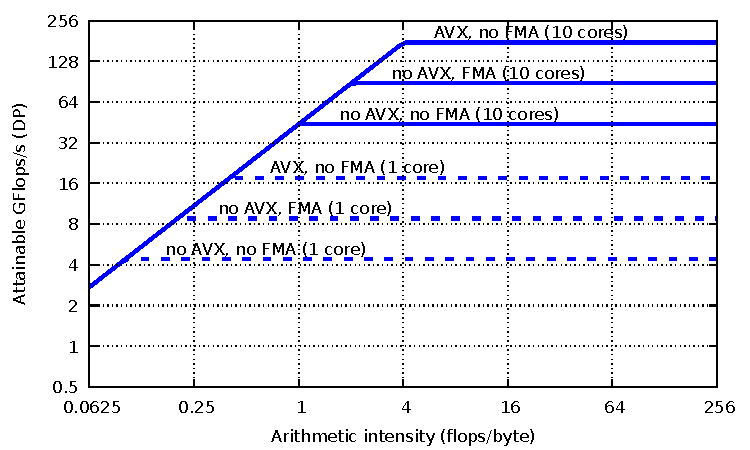
\includegraphics[width=0.7\textwidth,clip=true]{images/roofline/roofline_emmy_Xeon2660v2_core-ceilings.pdf}
   \caption{Berkeley Roofline model of Intel Xeon E5-2660 v2 with various in-core ceilings for 1 and 10 cores.}
  \label{fig:roofline_emmy_core-ceilings}
\end{figure}

\subsubsection*{Bandwidth Roofline Ceilings}

%\todop{
%prefetching?
%}

In Figure \ref{fig:mrm:bw-scaling} we can see memory bandwidth achieved by two Haswell processors (desktop and server) using a different number of cores. The desktop processor nearly saturates the bandwidth with one core, but the server processor achieves only about 40\% of bandwidth with a single core and needs at least 3 or 4 cores to fully saturate the bandwidth.

When data are transferred between memory and the L3 cache or different cache levels, they are always transferred in chunks called cache line. On Intel processors the size of cache line is usually 64\,B. Even if only 1\,B is needed, the whole cache line is transferred. Or when data are accessed with nonunit stride, some data are transferred and not used. This can lead to saturating the memory bandwidth while getting little useful data.

When NUMA is used, there is a memory controller at every NUMA domain. If all data are allocated on the same controller, this can happen, for example, by wrong first touch (initializing the data sequentially), then the other controllers are not used, lowering the bandwidth. Also when processes from one domain access data from another domain, the communication goes through a NUMA link between domains, which can become a bottleneck.

In Figure \ref{fig:roofline_emmy_memory-ceilings} we can see the effect of lower bandwidth when single core is used on the roofline model. As the bandwidth is lower, the corresponding line moves down. Note also the intersection of the horizontal and skewed line. It moved from arithmetic intensity 4\,F/B to about 16\,F/B, so a kernel that is compute bound on 10 cores could become memory bound on 1 core.

\begin{figure}[t]
   \centering
   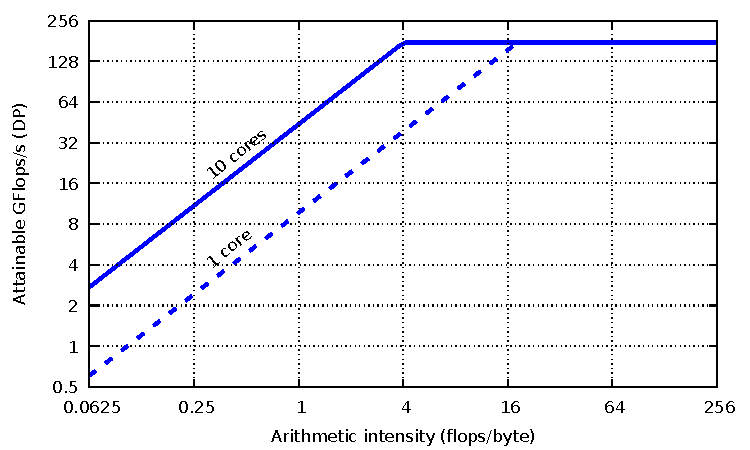
\includegraphics[width=0.7\textwidth,clip=true]{images/roofline/roofline_emmy_Xeon2660v2_memory-ceilings.pdf}
   \caption{Roofline model of Intel Xeon E5-2660 v2 with bandwidth ceilings for 1 and 10 cores.}
  \label{fig:roofline_emmy_memory-ceilings}
\end{figure}

As it is not possible reading data from memory using one thread and using all available threads for computations or vice versa, we can combine Figures \ref{fig:roofline_emmy_core-ceilings} and \ref{fig:roofline_emmy_memory-ceilings}. The roofline model with both in-core and bandwidth ceilings is shown in Figure \ref{fig:roofline_emmy_all-ceilings}.

\begin{figure}[t]
   \centering
   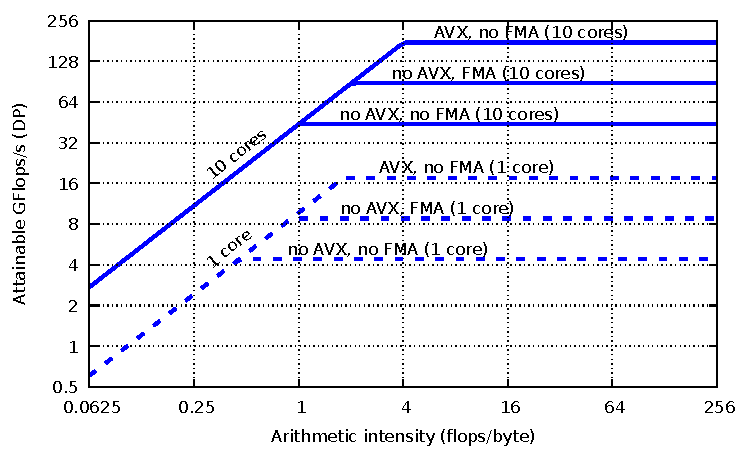
\includegraphics[width=0.7\textwidth,clip=true]{images/roofline/roofline_emmy_Xeon2660v2_all-ceilings.pdf}
   \caption{Roofline model of Intel Xeon E5-2660 v2 with both in-core and bandwidth ceilings.}
  \label{fig:roofline_emmy_all-ceilings}
\end{figure}

\begin{figure*}%
  \centering%
  
 \begin{tabular}{cc}
 %\begin{tabular}{>{\tiny \bfseries}lcccccccccc>{\tiny \bfseries}lccccccccccc}
 \multicolumn{1}{c}{\tiny \bfseries IVB} & \multicolumn{1}{c}{\tiny \bfseries
HSW-D} \\
  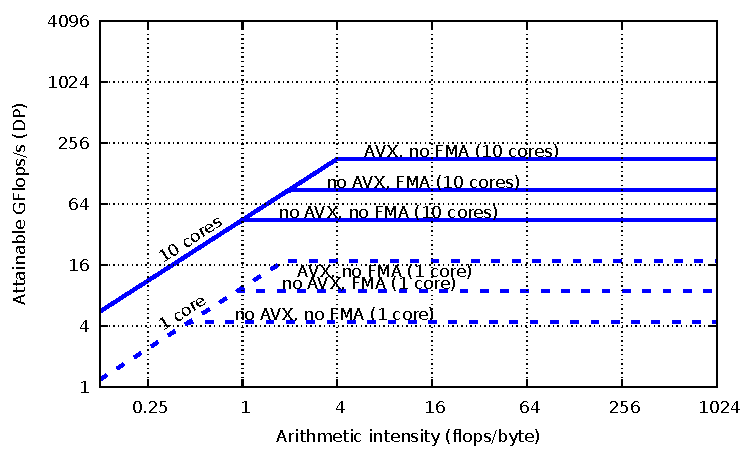
\includegraphics[width=0.49\textwidth,clip=true]{images/roofline/roofline_IVB.pdf}% 
  & 
  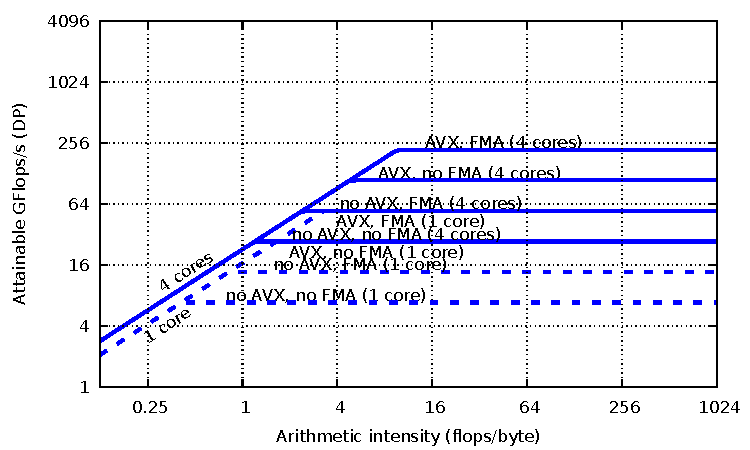
\includegraphics[width=0.49\textwidth,clip=true]{images/roofline/roofline_HSW-D.pdf}% 
  \\
  
\multicolumn{1}{c}{\tiny \bfseries HSW-S} & \multicolumn{1}{c}{\tiny
\bfseries BDW} \\
  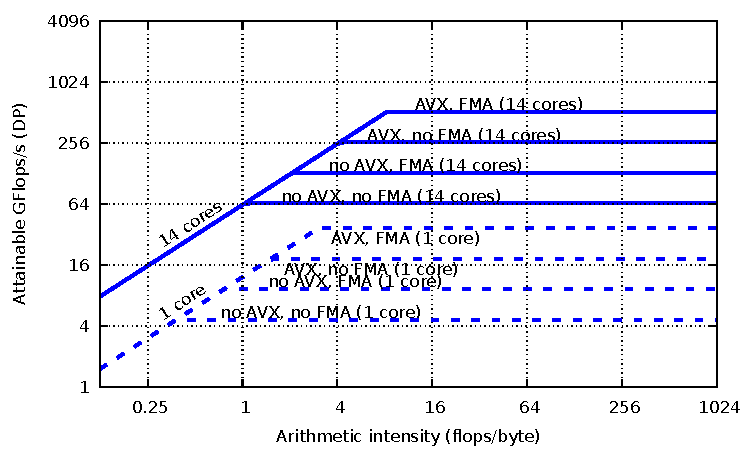
\includegraphics[width=0.49\textwidth,clip=true]{images/roofline/roofline_HSW-S.pdf}% 
  & 
  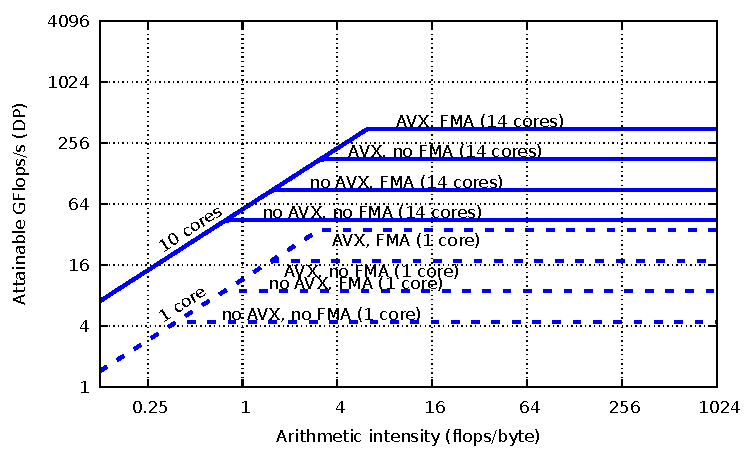
\includegraphics[width=0.49\textwidth,clip=true]{images/roofline/roofline_BDW.pdf}% 
  \\
  
\multicolumn{1}{c}{\tiny \bfseries SKX} &
\multicolumn{1}{c}{\tiny \bfseries KNL} \\
  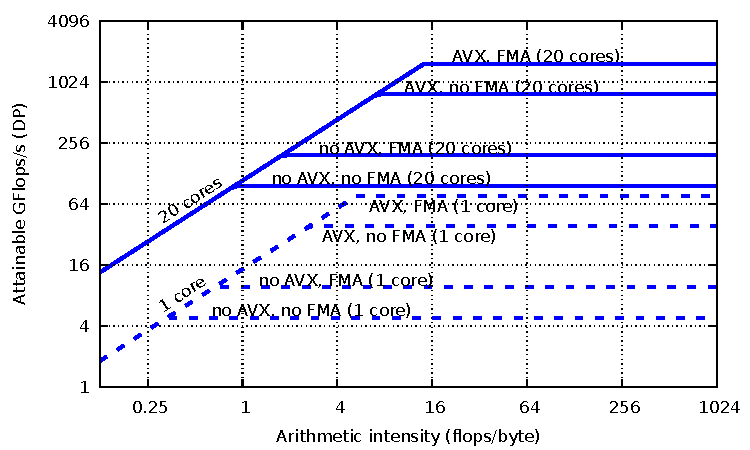
\includegraphics[width=0.49\textwidth,clip=true]{images/roofline/roofline_SKX.pdf}% 
  & 
  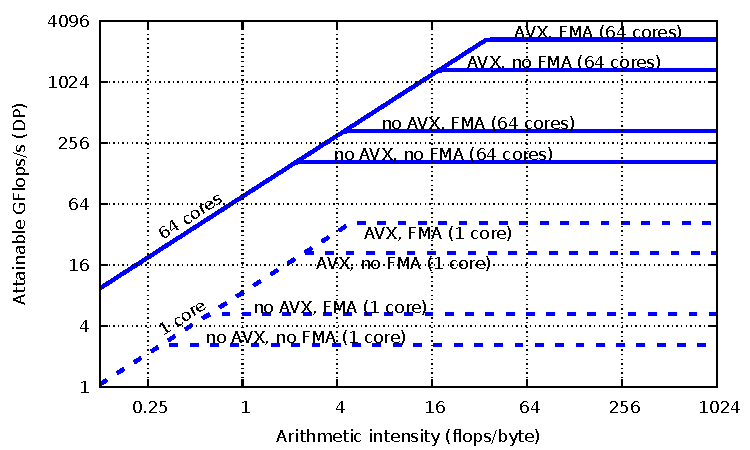
\includegraphics[width=0.49\textwidth,clip=true]{images/roofline/roofline_KNL.pdf}% 
  \\
  
\multicolumn{1}{c}{\tiny \bfseries
ZEN-D} & \multicolumn{1}{c}{\tiny \bfseries ZEN-S} \\
  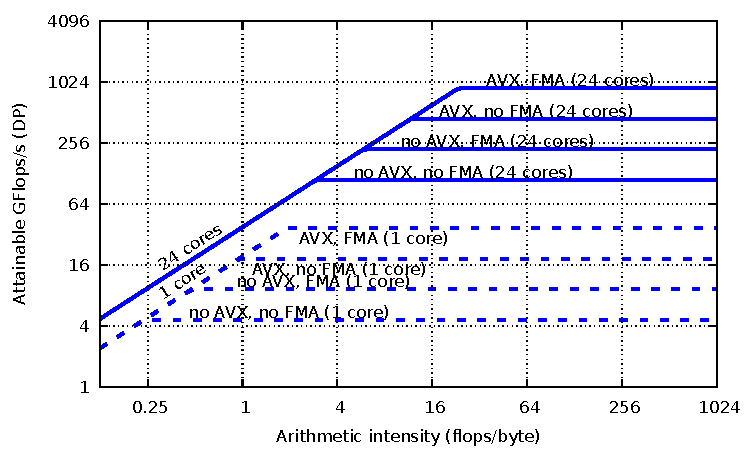
\includegraphics[width=0.49\textwidth,clip=true]{images/roofline/roofline_ZEN-S.pdf}% 
  & 
  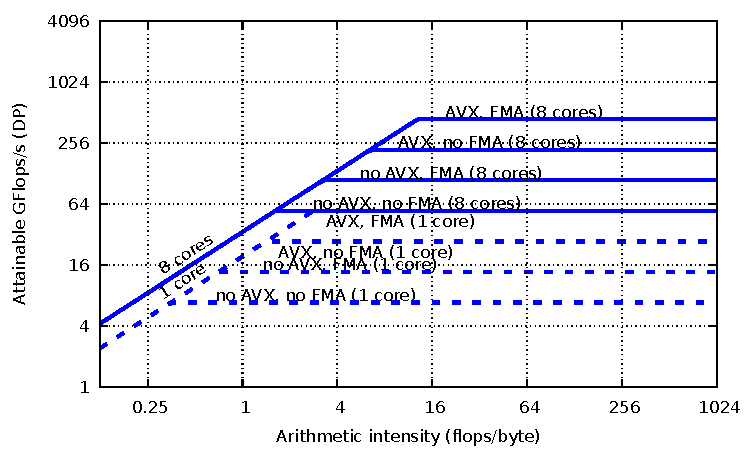
\includegraphics[width=0.49\textwidth,clip=true]{images/roofline/roofline_ZEN-D.pdf}% 
\\

\end{tabular}
%%
  %
  \caption{Roofline models of processors listed in Table \ref{tab:m:list}.}%
  \label{fig:rooflines}
\end{figure*}

%The Roofline model brings together two machine parameters describing possible bottlenecks, maximum performance $P_{max}$ and memory bandwidth $b_s$, and visualizes upper bound of performance any code can achieve on given machine.
%It is a graph with operational intensity $I$ on the x-axis and performance $P$ on the y-axis. The two bottlenecks are displayed as two lines:
%The horizontal line is a visualizaiton of attainable performance $P = P_{max}$.
%The skewed line is a function of memory bandwidth and operational intensity $P = I * P_{max}$.
%As these are the factors limiting the performance, we can expect performance of any program must be below these lines or in the best case on the lower of the two limits.
%We can write the performance upper bound as a function of either operational intensity or code balance as
%\begin{equation}
%   P = min(P_{max}, I \cdot b_s) = min(P_{max}, b_s / B_c).
%\end{equation}
%This can be visualized as \todol{ref naive graph}.
%The shape of the graph is what gives the model its name.
%
%Any compute kernel can be shown in the graph as a vertical line under the roofline. X-coordinate of the line is the operational intensity of the kernel.
%We can expect the performance of given kernel is somewhere along this line. Closer to the roofline (higher) is better, but the it can never exceed the roofline.
%
%The point where the two lines intersect is at operational intensity $I = B_m^{-1}$. At this point the performance $P_{max}$ is achieved while reading and writing to memory as much as possible, $b_s$\,B/s.
%Performance of any kernel on the right side of this point ($B_c < B_m$ or $I > B_m^{-1}$) is limited by $P_{max}$. We call such kernel compute bound.
%Performance of any kernel on the left side of this point ($B_c > B_m$ or $I < B_m^{-1}$) is limited by $b_s$. We call such kernel memory bound.
%
%%\todop{
%%\begin{itemize}
%%    \item naive, ceilings
%%    \item cite williams
%%\end{itemize}
%%}
%
%\begin{figure}[H]
%   \centering
%   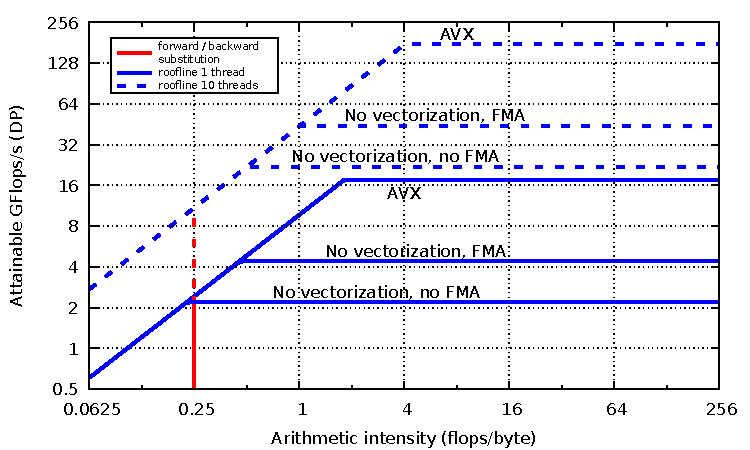
\includegraphics[width=0.7\textwidth,clip=true]{images/roofline_emmy_Xeon2660v2}
%   \caption{Roofline model of the  Intel Xeon E5-2660 v2 CPU.}
%  \label{fig:roofline_emmy}
%\end{figure}
%
%
%%\todop{
%%\begin{itemize}
%%    \item Description of CPU
%%    \item Memory hierarchy
%%\end{itemize}
%%}

\section{Erlangen Execution-cache-memory model}
\label{sec:ecm}

The Roofline model is a simple model
for performance prediction in the saturated case.
Hereby it is assumed code is limited by floating point performance or by the
memory bandwidth.
The ECM performance model (\cite{treibig-2010-ecm,hager-2012-ecm}) is a refinement
of the Roofline model.\footnote{For further details regarding the ECM model refer
to~\cite{stengel-2015}.}
In contrast it allows a performance prediction on the single core level as well
as a scaling prediction over the socket.
The model takes into account the duration of the code execution inside the core
separated by arithmetic and data movement.
Furthermore data transfers in the memory/cache hierarchy are considered as well
as the achievable memory bandwidth.
%
Finally both parts build the single core model, which is used to determine the
scaling behavior over the cores until a bottleneck is reached. 
%
For memory bound codes this is typically the achievable memory bandwidth, \todol{which represents the bottleneck ..}  as all
other infrastructures like Intel's L3 cache on Ivy Bridge, Haswell, and Broadwell
scale perfectly. 

The ECM model has some restrictions on the code to be analyzed.
It is important that streaming accesses are performed. This means prefetching
works perfectly and can hide latency effects.
The ECM model predicts the number of CPU cycles (cy) required to execute a certain number of iterations of a given loop on a single core. Since the smallest amount of data transferred between cache levels is one cache line (CL), it is a reasonable unit of work for the predictions. The size of cache line on Intel processors is 64\,B, which is for streaming kernels 8 iterations with floating point numbers in double precision.

To construct the model, we consider two parts separately: the in-core execution, assuming all data were already fetched to the L1 cache and there are no cache misses, and the time to fetch the data from its location to the L1 cache.
 %the main memory or the cache level where it is assumed to be stored

\subsection*{In-core execution}

To determine the in-core execution time, a simple model for instruction throughput on the given architecture is required. Figure \ref{fig:hsw-microarch} shows a port model for the Intel Haswell architecture. The port scheduler schedules instructions to ports independently out of program order, making sure all data dependencies are met.

Instructions inside ports are pipelined, but only one instruction per port can
be issued per cycle.
Haswell can perform two loads (LD, ports~$2D$ and~$3D$) and one store (ST,
port~$4$) of sizes up to $32$\,B at the same time (\cite{intel-orm-2016}), each.
Each load and store requires an address to be generated by an address
generation unit (AGU, ports~$2$,~$3$, and~$7$).
However on port~$7$ only a simple AGU is located, which is limited to simple
addressing modes\footnote{AGUs on port 2 and 3 support addressing "base plus index plus offset", AGU on port 7 supports only simple addressing mode "base plus offset".}~(\cite{intel-orm-2016,hofmann-2016-hsw}).
%
For floating point operations, the cores host two 
FMA units (port~$0$ and~$1$), two multiplication (MUL) units (port~$0$
and~$1$), and one add (ADD) unit (port~$1$).

\todol{Example of distribution of the instructions over the ports is found in
Figure~\ref{fig:daxpy:ecm}. ... probably drop}
For the ECM model the duration of the execution inside the core is split into
two categories.
The first one comprises only data movement between registers and the L1 cache,
i.\,e.,\ loads and stores occurring on port~$2D$,~$3D$, and~$4$.
The second category consists of the rest, which can possibly overlap with the
loads and stores, like arithmetic, logic, and address generation.
The execution in-core time $T_{core}$ is set to the time of the port with the longest execution time.

\subsection*{Data transfers through the memory hierarchy}

Data that are not present in the L1 cache must be fetched from lower levels and modified data evicted to make room for new cache lines.
On Intel architectures, transfer of one cache line between adjacent cache levels takes 2 cycles.
Transfer time of one 64\,B cache line can be computed knowing the memory bandwidth $b_s$ and clock frequency $f$ as $64*f/b_s$ cycles.

As $b_s$, one could take the nominal memory bandwidth.
However, this bandwidth is practically never reached and depends strongly on the
access pattern used.
This is caused by the organization of the memory subsystem, where e.\,g.,\ banking
conflicts and DRAM page misses impair performance.
With detailed knowledge about the internals of the memory controller
(scheduling strategies, thresholds for strategy switching, ...) and DRAM modules
this could also be modeled, which is far from being trivial (\cite{jacob-2007}).
As this is beyond the scope of the ECM model, typically, a microbenchmark
resembling the used access pattern by the code under investigation is used
to measure the attainable bandwidth and use it as input for the model.

\section{ECM Model Application}
\label{sec:ecm-application}

\subsection{DAXPY vector addition}
\label{sec:epm}

%{\color{blue} juraj: what are the limitations of the roofline? e.g. cannot model bottlenecks beyond peak perf. or memory bandwidth (useful paper https://dl.acm.org/doi/pdf/10.1145/2751205.2751240); short discussion about where Roofline/ECM models were applied and how accurate they predicted the performance compared to experimental measurements; before introducing ECM you probably need to write something about cache hierarchy and instruction pipelines, load/store instructions and their latency/throughput}

In the following text we give a brief introduction to the ECM model by analyzing a
simple daxpy-like kernel on the HSW-S system, whose processor is based on the Intel Haswell
microarchitecture. The daxpy kernel to be analyzed is
%
\begin{lstlisting}
for (int i = 0; i < N; ++i) 
  r[i] +=  s * l[i];
\end{lstlisting}
%
The vectors \verb'r' and \verb'l' are double-precision floating point vectors
with \verb'N' elements each. 
%The \verb'index' vector consists of $4$\,B integers.
Furthermore \verb's' is a scalar double-precision floating point variable.
%
The code is vectorized via AVX and FMA3 instructions by the compiler and
additionally $4$-way unrolled to reach full performance.
The unrolled code becomes
\begin{lstlisting}
for (int i = 0; i < N; i += 4)
{
  r[i  ] +=  s * l[i  ];
  r[i+1] +=  s * l[i+1];
  r[i+2] +=  s * l[i+2];
  r[i+3] +=  s * l[i+3];
}
\end{lstlisting}
%Effectively one iteration of the compiler
%generated loop performs $16$ iterations of the original kernel.
%
For easier modeling, we take as many iterations into account as are needed to
process a whole cache line\footnote{On Intel architectures, the length of the cache line is 64\,B.}.
Hence, for the daxpy kernel with double-precision floating point numbers the
work package we model is eight iterations (or two iterations of the unrolled loop).
%
To process these eight iterations with AVX and FMA3, four $32$\,B AVX loads (\verb|r[:]| and
\verb|l[:]|), two
$32$\,B AVX stores (\verb'r[:]'), and two FMAs are required.
%
Hereby we define the ``work'' performed by eight iterations is to transfer $W = 192$\,B.
%
In order to determine the duration of the execution of the code inside
the core we assume all operands reside in the L1 cache.

%\begin{figure}[tp]
%  \centering
%  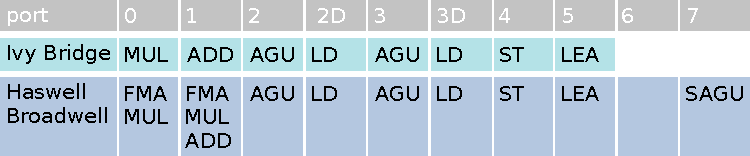
\includegraphics[width=0.49\textwidth,clip=true]{images/IntelMicroArchPorts}
%  \caption{Ports and associated execution units of Intel microarchitectures.
%Only the units relevant for this paper are shown.}
%  \label{fig:ports}
%\end{figure}

The duration of the in-core execution depends on the core's architecture.
For HSW-S it's the Haswell microarchitecture.
The superscalar design has several ports with different execution units for
different types of instructions, shown as part of Figure~\ref{fig:hsw-microarch}.
Instructions scheduled to different ports run independently.
The instruction scheduler takes care that no data dependencies are violated.

\begin{figure}[t]
  \centering
  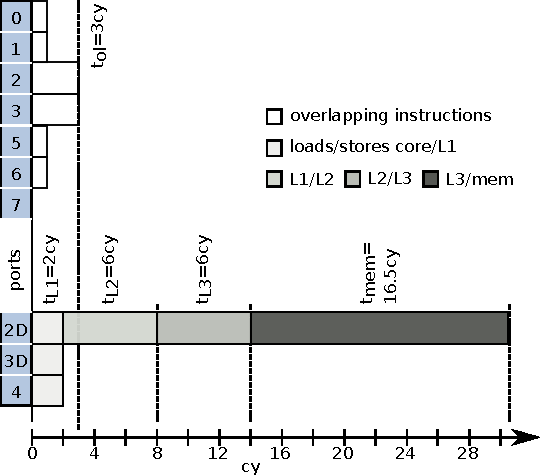
\includegraphics[width=0.42\textwidth,clip=true]{images/ecm-hsw-daxpy}
  \caption{Run time contributions of different execution ports and cache/memory
hierarchy levels for eight iterations of the daxpy kernel on HSW-S (Haswell micro-architecture). It seems that the simple AGU on port~$7$ is not used and all the addresses are generated on ports~$2$ and~$3$.}
  \label{fig:daxpy:ecm}
\end{figure}

\begin{figure}[t]
  \centering
  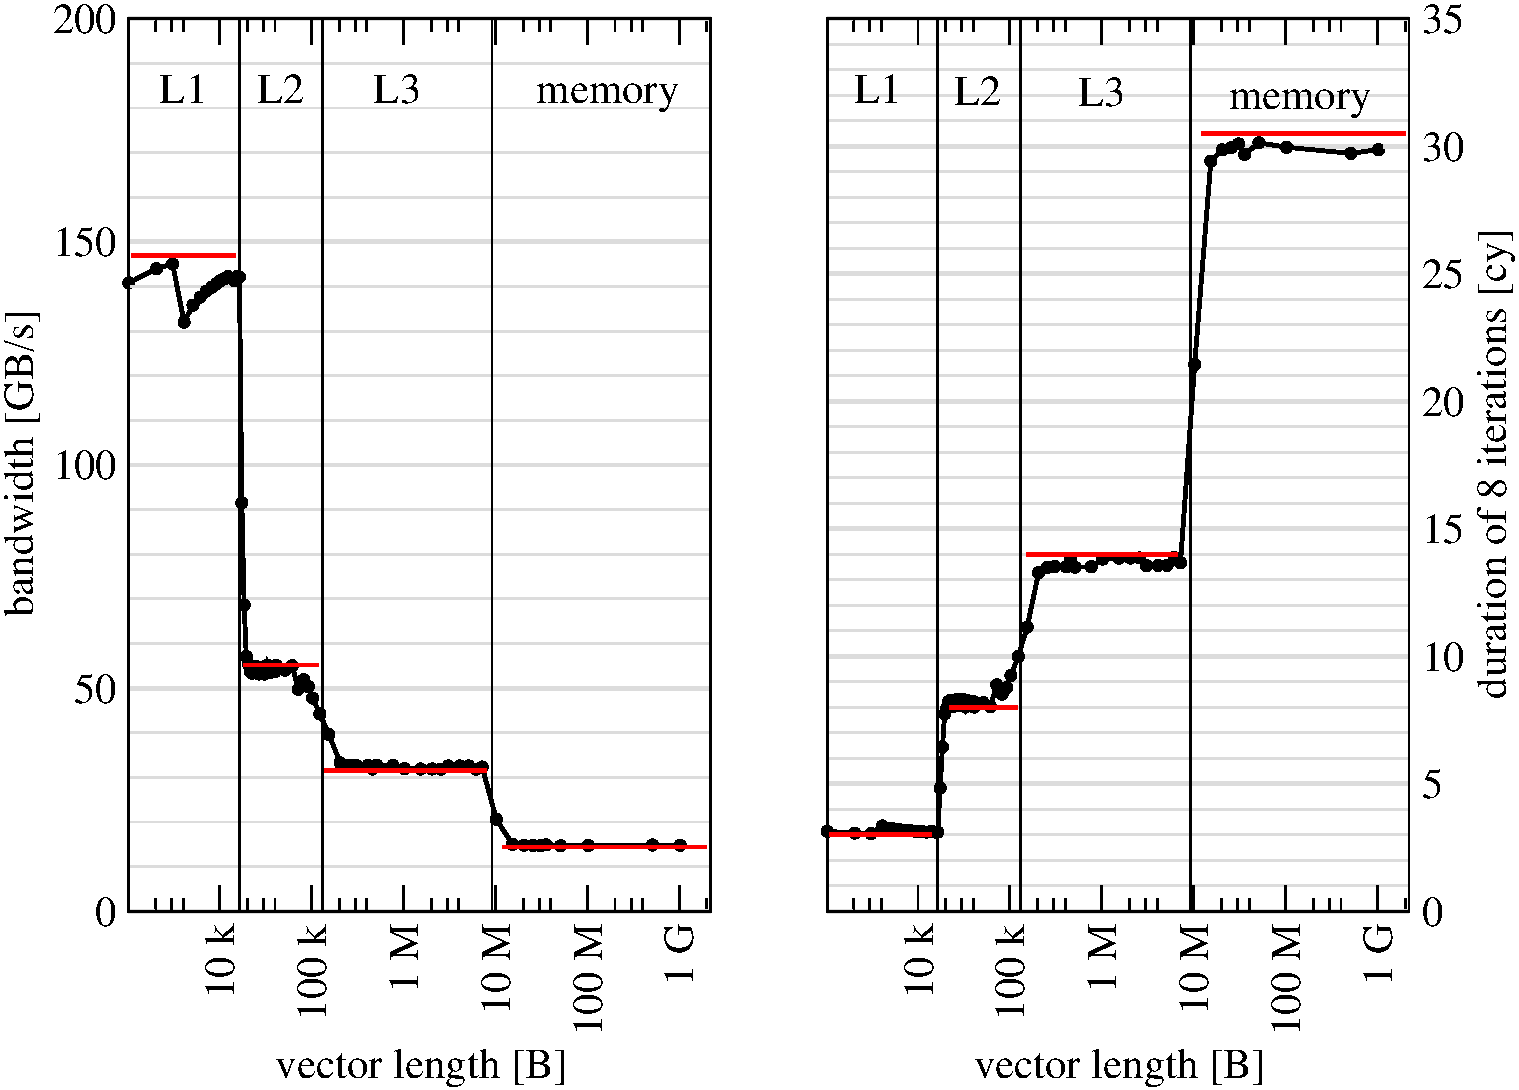
\includegraphics[width=0.60\textwidth,clip=true]{images/daxpy-bw-hasep1-f-2_3-w-cy}
  \caption{Bandwidth and duration of 8 iterations, i.\,e.,\ two iterations of the
compiler generated loop, for the daxpy kernel on HSW-S. Note that the total
working set required for vectors
\protect\texttt{r} and \texttt{l} is twice the AVX vector length.}
  \label{fig:daxpy:perf}
\end{figure}

%We could manually analyze the assembly code of the daxpy kernel and create a
%scheduling of the instructions onto the ports to determine the duration of the
%execution inside the core.
%This is not feasible for complex kernels and often requires internal knowledge
%of the core, which is publicly not available.
%Instead we use Intel's Architecture Code Analyzer (IACA) (\cite{intel-iaca})
%for this task.
%We use the tool's throughput mode, where it is assumed that iterations of the
%loop are independent and can overlap due to the out-of-order engine.
%Further we assume no pipeline bubbles of the different ports.
Haswell can perform two loads (port $2D$ and $3D$) and one store (port $4$) of
sizes up to $32$\,B at the same time~(\cite{agner-2016-11-3}).
This constellation requires the store address to be simple addressing as only in
this case the address generation unit (AGU) on port~$7$ can be used.
% Effectively this boils down to either two loads or one load and store.
%
For floating point operations relevant, it hosts two FMA units (port 0 and
1) two MUL units (port 0 and 1), and one ADD unit (port 1).

Under this considerations two iterations of the compiled loop would require $1$\,cy
for the FMA (port $0$ and $1$), $2$\,cy for the four AVX loads (port $2$ and $3$),
and $2$\,cy for the four AVX stores (port $4$).
$6$ addresses need to be generated.
This takes $2$\,cy, if the simple AGU on port $7$ is used.
Instructions regarding index counter increments are for this case negligible, hence we ignore them.
The distribution of the instructions over the ports is found in Figure~\ref{fig:daxpy:ecm}.

For the ECM model the duration of the execution inside the core is split into
two categories.
The first one comprises only data movement between registers and L1 cache,
i.\,e.\ loads, stores occurring and address generation.
The second category consists of the rest, which can possibly overlap with the
loads and stores, like arithmetic, logic.
%We classify the ports into arithmetic/logic (port $0$, $1$, $5$, and $6$) and
%data movement (port $2$, $3$, $4$, and $7$).
The maximum duration $t_\text{L1}$ of the first class (port $2$, $3$, $4$, and $7$) is
\be
  t_\text{L1} = 2\,\cyw.
\ee
The maximum duration of the latter class (port $0$, $1$, $5$, and $6$), $t_\text{ol}$, is
\be
  t_\text{ol} = 1\,\cyw
\ee
%
(normalized to eight iterations) as the maximum duration on the ports overlapping with data
movements.
%
%Note that the compiler uses simple addressing for store addresses, which
%according to IACA will utilize the simple AGU on port~$7$.
%
%
The performance $P_\text{L1}$, when all data are fetched from L1, is then
computed as 
%
\be
  P_\text{L1} = \frac{W}{\max(t_\text{ol}, t_\text{L1})} f,
\ee
%
where $W$ denotes the loop specific work performed and $f$ clock
frequency of the core.
For this loop with $W=192$\,B and $f=2.3$\,GHz we have $P_\text{L1} =
220.8$\,GB/s. 
Measurements shown in Figure~\ref{fig:daxpy:perf} reveal that only around
$145$\,GB/s are reached.
If the simple AGU on port~$7$ is not used, the store addresses are
generated by the two remaining AGUs.
This causes $t_\text{ol}$ to be increased by $1$\,\cyw{} and becoming the new
bottleneck.
This results in a corrected
%
\be
   t_\text{ol} = 3\,\cyw
\ee
%
with $P_\text{L1} = 147.2$\,GB/s, which is in line with the measurements as shown in Figure~\ref{fig:daxpy:perf}.


Modeling the performance when data reside in different cache levels from L1
requires analyzing data transfers between these levels.
For daxpy this is straightforward as vectors \verb'r' and \verb'l' are
streamed from/to memory and no cache reuse takes place.
Throughout the cache/memory hierarchy we transfer between each cache level three 
cache lines (cl) for each iteration: load $1$\,cl of \verb'l', load $1$\,cl of
\verb'r', and store $1$\,cl of \verb'r'.

Transferring a cache line between L1/L2 and L2/L3 takes $2$\,cy each.
Hence it takes
%
\be
  t_\text{L2} = 6\,\text{cy} \qquad \text{and} \qquad t_\text{L3} = 6\,\text{cy}
\ee
%
to transfer our three cache lines, respectively.
For computing the performance $P_\text{L2}$ and $P_\text{L3}$, when data resides
in the L2 or L3 cache, respectively, we have to add $t_\text{L2}$ and $t_\text{L3}$
to the duration of the data path, as on the considered Intel architectures data
transfers seem be be serialized when streaming accesses occur.\footnote{This need
not be the actual implementation inside the architecture; it only resembles
the observation and can be different on other architectures.}
The performance is then
%
\begin{align}
  P_\text{L2} &= \frac{W}{\max(t_\text{ol}, t_\text{L1} + t_\text{L2})} f, \\
  P_\text{L3} &= \frac{W}{\max(t_\text{ol}, t_\text{L1} + t_\text{L2} +
t_\text{L3})} f.
\end{align}
%
In our case $P_\text{L2} = 55.2$\,GB/s and $P_\text{L3} = 31.5$\,GB/s.
%

%How many cache lines per cycle can be transferred between L3 and memory could
%theoretically be obtained by taking the nominal memory bandwidth into account.
%However, this bandwidth is practically never reached and depends strongly on the
%access pattern used.
%This is caused by the organization of the memory subsystem, where e.\,g.\ banking
%conflicts and DRAM page misses incur performance.
%With detailed knowledge about the internals of the (closed IP) memory controller
%(scheduling strategies, thresholds for strategy switching, ...) and DRAM modules
%this could also be modeled, which is far from being trivial~\cite{jacob-2007}.
%As this is beyond the scope of the ECM model typically a micro benchmark
%resembling the used access pattern by the code under investigation is used
%to measure the attainable bandwidth and use it as input for the model.
%%
%For this model we use \textsc{McCalpin's} STREAM copy
To determine the memory bandwidth we use \textsc{McCalpin's} STREAM copy
benchmark (\cite{mccalpin-1995}) which achieves (without nontemporal stores and
including the write allocate) a bandwidth of $\approx 26.9$\,GB/s when all cores
of a cluster are utilized\footnote{When Cluster-on-Die (COD) is enabled, the cores are split into two NUMA domains. The HSW-S processor has 14 cores, that are split in two NUMA domains, each with 7 cores.}.
With the core's clock frequency of $2.3$\,GHz it takes $5.5$\,cy to transfer one
cache line between L3 cache and memory.
Transferring our three cache lines between these two levels takes then
%
\be
  t_\text{mem} = 16.5\,\text{cy}.
\ee
%
The performance $P_\text{mem}$, when every vector is streamed from memory, is then
%
\be
  P_\text{mem} = \frac{W}{\max(t_\text{ol}, t_\text{L1} + t_\text{L2} +
t_\text{L3} + t_\text{mem})} f.
\ee
%
This leads to $P_\text{mem} = 14.5$\,GB/s. 

\subsection{Indirect DAXPY}
\label{sec:ecm-indirect-daxpy}

Indirect DAXPY is similar to the code analyzed in section \ref{sec:epm}, with the difference of indirect access \verb|idx| to the vector \verb|r|.

%
\begin{lstlisting}
for (int i = 0; i < N; ++i) 
  r[idx[i]] +=  s * l[i];
\end{lstlisting}
%
The vectors \verb'r' and
\verb'l' are double-precision floating point vectors with \verb'N' elements
each. 
The \verb'idx' vector contains $4$~B integers.
Furthermore \verb's' is a scalar double precision floating point variable.
%
The code is 4-way unrolled and by the compiler, when
optimizations are turned on and target ISA is AVX2 and FMA3. One iteration
over this newly formed loop now performs 4 scalar iterations. The code snipped
from above effectively becomes
%
\begin{lstlisting}
for (int i = 0; i < N; i += 4)
{
  r[idx[i  ]] += s * l[i  ];
  r[idx[i+1]] += s * l[i+1];
  r[idx[i+2]] += s * l[i+2];
  r[idx[i+3]] += s * l[i+3];
}
\end{lstlisting}
%
For the ECM model we determine the duration of the execution of the code inside
the core under the assumption all operands reside in L1 cache.

\begin{figure}[t]
  \centering
  \includegraphics[width=0.56\textwidth,clip=true]{images/ecm-hsw-daxpy-indirect}
  \caption{Run time contributions of different execution ports and cache/memory
hierarchy levels for eight iterations of the indirect daxpy kernel on HSW-S (Haswell micro-architecture).}
  \label{fig:daxpy-indirect:ecm}
\end{figure}

\begin{figure}[t]
  \centering
  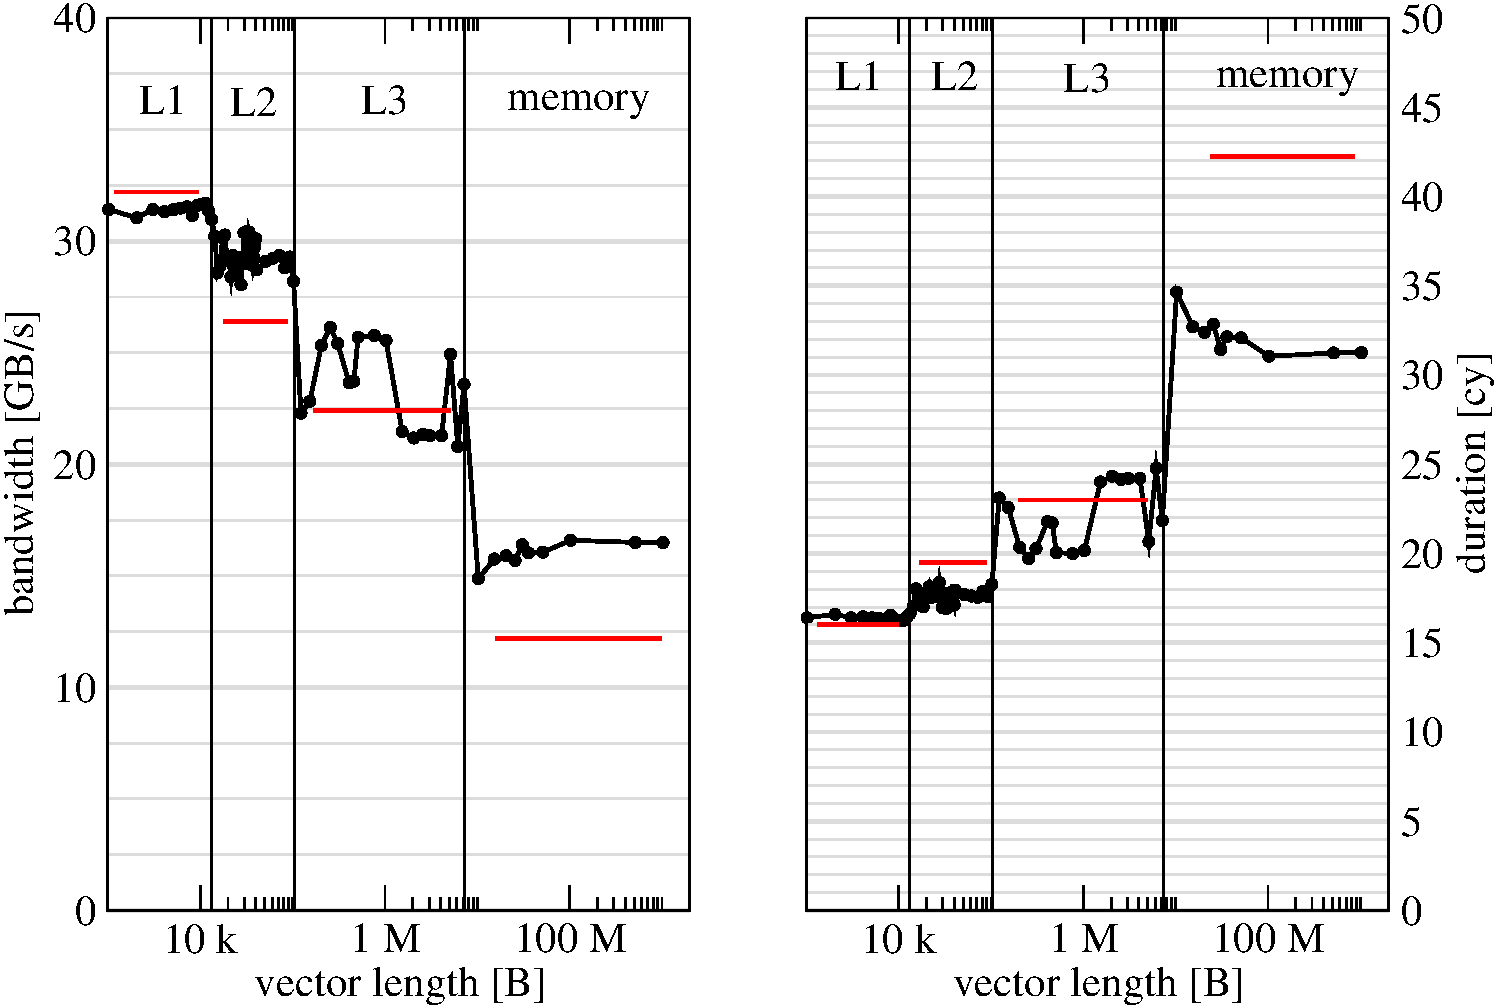
\includegraphics[width=0.60\textwidth,clip=true]{images/daxpy-indirect-bw-hasep1-f-2_3-w-cy}
   \caption{Bandwidth and duration of 8 iterations, i.\,e.,\ two iteration of the
compiler generated loop, for the indirect daxpy kernel on HSW-S.}
  \label{fig:daxpy-indirect:perf}
\end{figure}

Eight iterations of the loop (or two iterations of the unrolled loop) require
sixteen $8$\,B loads (\verb|r[:]| and
\verb|l[:]|), eight $4$\,B loads (\verb'idx[:]'), eight
$8$\,B stores (\verb'r[:]'), and $32$ address generations.
Furthermore eight scalar fused-multiply-adds are used. 
We define the work performed by eight iterations of the loop (or two iterations of compiler unrolled loop) to be $W =
224$\,B.

How long the execution takes depends on the underlying architecture. 
In order to determine this, we take a look at the Intel Haswell
microarchitecture in Fig.~\ref{fig:hsw-microarch}.
The super-scalar design has several ports with different execution units for
different types of instructions.
Instructions scheduled to different ports run independently.
The instruction scheduler takes care that no data dependencies are violated.
Instructions inside ports are pipelined, but only one instruction per port can
be issued per cycle.
Haswell can perform two loads (port $2D$ and $3D$) and one store (port $4$) of
sizes up to $32$\,B at the same time~(\cite{agner-2016-11-3}).
This constellation requires the store address to be simple addressing as only in
this case the address generation unit (AGU) on port~$7$ can be used.
% Effectively this boils down to either two loads or one load and store.
%
For floating point operations relevant, it hosts two FMA units (port 0 and
1) two MUL units (port 0 and 1), and one ADD unit (port 1).

Under this considerations two iterations of the compiled loop would require $4$\,cy
for the FMA (port $0$ and $1$), $12$\,cy for the twenty four loads (port $2$ and $3$),
and $8$\,cy for the eight stores (port $4$).
$32$ addresses need to be generated. We assume the simple AGU on port $7$ is not used, as we observed for DAXPY (section \ref{sec:epm}). Generating all $32$ addresses on AGUs on ports $2$ and $3$ requires $16$\,cy.
Instructions regarding index counter increments are for this case negligible, hence we ignore them.
%From the $32$ address generation four are simple an can run on the simple AGU on
%port $7$ requiring $4$\,cy, whereas the remaining $28$ addresses are handled in
%$14$\,cy due to two AGUs on port $3$ and $4$.
We assume that the out-of-order engine can fill bubbles in the pipelines of the
different ports as the loop iterations are independent of each other.
We classify the ports into arithmetic/logic (port $0$, $1$, $5$, and $6$) and
data movement (port $2$, $3$, $4$, and $7$). 
The maximum duration $t_\text{ol}$ of the first class of ports is 
%
\be
  t_\text{ol} = \max(4\,\cyw, 4\,\cyw, 6\,\cyw, 6\,\cyw)
= 6\,\cyw
\ee
%
and the maximum duration of the data movement ports $t_\text{L1}$ which
load/store data from/to L1 is
\be
%  t_\text{L1} = \max(12\,\cyw, 14\,\cyw, 8\,\cyw, 4\,\cyw) =
  t_\text{L1} = \max(16\,\cyw, 16\,\cyw, 8\,\cyw, 0\,\cyw) =
16\,\cyw.
\ee
%
% for the duration of the data transfers between core and L1 cache.
%
The performance $P_\text{L1}$, when all data is fetched from L1, is then computed as 
%
\be
  P_\text{L1} = \frac{W}{\max(t_\text{ol}, t_\text{L1})} f,
\ee
%
where $W$ denotes the loop specific work performed and $f$ clock frequency of the core.
For this loop with $W=224$\,B and $f=2.3$\,GHz we have $P_\text{L1} =
32.2$\,GB/s,
%On HSW1 only $\approx 31$\,GB/s, i.\,e.\ 80\,\% of the predicted
%performance are achieved for this loop, shown in
which is in line with the measurements in
Figure~\ref{fig:daxpy-indirect:perf}.

Modeling the performance when data resides in different cache levels from L1
requires to analyse the data transfers between these levels.
In this case this is straight forward as vector \verb'r', \verb'l', and
\verb'idx' are streamed from/to memory and no cache reuse takes place.
Throughout the cache/memory hierarchy we transfer between each cache level
$224$\,B $= 3.5$\,cl (cache lines) for each iteration: load $64$\,B of
\verb'l', load $64$\,B of \verb'r', load $32$\,B of \verb'idx' and store $64$\,B
of \verb'r'.

Transferring a cache line between L1/L2 and L2/L3 takes $1$\,cy (\cite{intel-orm-2016}). Hence it takes
%
\be
  t_\text{L2} = 3.5\,\cyw\ \text{and}\ t_\text{L3} = 3.5\,\cyw
\ee
%
to transfer our $224$\,B.
For computing the performance $P_\text{L2}$ and $P_\text{L3}$, when data resides
in L2 or L3 cache, respectively, we
have to add $t_\text{L2}$ and $t_\text{L3}$ to the duration of the data path, as on the considered
Intel architectures data transfers seem be be serialized when streaming accesses
occur\footnote{This need not to be the actual implementation inside the
architecture, it only resembles the observation and can be different on other
architectures.}.
The performance is then
%
\begin{align}
  P_\text{L2} &= \frac{W}{\max(t_\text{ol}, t_\text{L1} + t_\text{L2})} f, \\
  P_\text{L3} &= \frac{W}{\max(t_\text{ol}, t_\text{L1} + t_\text{L2} +
t_\text{L3})} f.
\end{align}
%
%In our case $P_\text{L2} = 29.4$\,GB/s and $P_\text{L3} = 18.2$\,GB/s.
In our case $P_\text{L2} = 26.4$\,GB/s and $P_\text{L3} = 22.4$\,GB/s.
%

How many cache lines per cycle can be transferred between L3 and memory could
theoretically be obtained by taking the nominal memory bandwidth into account.
However, this bandwidth is practically never reached and depends strongly on the
access pattern used.
This is caused by the organization of the memory subsystem, where e.\,g.\ banking
conflicts and DRAM page misses incur performance.
With detailed knowledge about the internals of the memory controller
(scheduling strategies, thresholds for strategy switching, ...) and DRAM modules
this could also be modeled, which is far from being trivial (\cite{jacob-2007}).
As this is beyond the scope of the ECM model typically a micro benchmark
resembling the used access pattern by the code under investigation is used
to measure the attainable bandwidth and use it as input for the model.
%
For this model we use \textsc{McCalpin's} STREAM copy
benchmark~(\cite{mccalpin-1995}) which achieves (without nontemporal stores and
including the write allocate) a bandwidth of $\approx 26.9$\,GB/s when all seven cores
of a cluster are utilized.
With the core's clock frequency of $2.3$\,GHz it takes $5.5$\,cy to transfer one
cache line between L3 cache and memory.
Transferring our $224$\,B between these to levels takes
%
\be
%  t_\text{mem} = 9.625\,\cyw.
  t_\text{mem} = 19.25\,\cyw.
\ee
%
The performance $P_\text{mem}$, when every vector is streamed from memory, is then
%
\be
  P_\text{mem} = \frac{W}{\max(t_\text{ol}, t_\text{L1} + t_\text{L2} +
t_\text{L3} + t_\text{mem})} f.
\ee
%
%This leads to $P_\text{mem} = 10.2$\,GB/s. 
This leads to $P_\text{mem} = 12.2$\,GB/s. 
\todol{Which is about 13\,\% less than the achieved performance on HSW-S architecture.}

%% The required information on the hardware capabilities can be obtained from the
%% data sheets of the vendors or measured via micro-benchmarks.
%% For good estimates regarding achievable memory bandwidth a benchmark which
%% exhibits the same access pattern as the code under investigation is preferable.
%% %
%% In our case primarily the nonzeros from matrix $L$ out of the \vlnz{}
%% array are loaded from memory.
%% Hereby we neglect, that for each panel also the indices into the right hand side
%% $r$ must be loaded. 
%% This seems to be a fair assumption for matrices with large panel sizes, like the
%% dense\footnote{MW: here already reference to the dense matrix} matrix with $n_p = 80$.
%% Here only for the panel's first column, indices must be loaded from memory
%% and can be $79$ times reused.
%% Further we ignore that during forward substitution stores to $r$ occur.
%% %
%% The most simple benchmark, which resembles this behavior, is linearly reading
%% from memory.
%% We accomplish this by summing up the elements of a vector $a$ which is large
%% enough to reside in memory: \texttt{s = s + a[i]}.
%% Note that the single core bandwidth for read only is below the STREAM copy
%% bandwidth (\texttt{a[i] = b[i]}).
%% Here \textsc{McCalpin} identifies limited concurrency as the
%% bottleneck\footnote{Comment of \textsc{McCalpin} in the Intel Forum found under
%% \texttt{http://software.intel.com/en-us/forums/topic/456184}.}.
%% However in the saturated case a higher bandwidth compared to STREAM copy is
%% achieved.
%% Through an $n$-way unrolling over columns
%% (described in section~\ref{sec:pm:dt:wu}) there are effectively $n$ concurrent
%% read streams for each core.
%% For simplicity we ignore the fact that with $n > 1$ possibly the attainable
%% bandwidth decreases.
%% %
%% Table~\ref{tab:hw} contains all the ECM model parameters used for the different
%% hardware systems.
%% 

\chapter{Node-level performance modeling of sparse triangular solve}
\label{c:modeling}

Even in scientific computing, simulation code development often lacks a basic understanding of performance bottlenecks and relevant optimization opportunities. In this chapter we will use a structured model-based performance engineering approach on the compute node level for a fundamental kernel operation in sparse factorization solvers. We aim at a deep understanding of how code performance comes about and which hardware bottlenecks might apply. The pivotal ingredient of this process is a performance model which links software requirements with hardware capabilities. Such models are often simplified such as the well-known Berkeley roofline model or the Erlangen ECM model, but it leads to deeper insights and strikingly more accurate runtime predictions.

The package PARDISO\footnote{A discussion of the algorithms used in
PARDISO, the user manual, and more information on the solver can be found at
\url{http://www.pardiso-project.org}}
is a thread-safe, high-performance, and memory-effi\-cient,
serial and parallel solver for the direct solution of unsymmetric
and symmetric sparse linear systems on shared memory multiprocessors.
The solver uses a combination
of left- and right-looking Level-3 BLAS supernode techniques
(\cite{AndBBDDDGHMOS99}).
In order to improve sequential and parallel sparse
numerical factorization performance, the algorithms are based on
a Level-3 BLAS update and pipelining parallelism is exploited with
a combination of left- and right-looking supernode techniques.

PARDISO calculates the solution of a set of sparse linear equations
with multiple right-hand sides, using a parallel $LU$, $LDL^T$, or $LL^T$
factorization. PARDISO supports a wide range of sparse matrix types and
computes the solution of real or complex,
symmetric, structurally symmetric or unsymmetric, positive definite,
indefinite or Hermitian sparse linear system of equations on shared-memory
multiprocessing architectures.

The parallel pivoting methods for unsymmetric matrices allow complete supernode pivoting in order to ensure numerical stability and scalability during the factorization process. For sufficiently large problem sizes numerical experiments demonstrate that the scalability of the parallel algorithm is nearly independent of the shared-memory multiprocessing architecture and a speedup of up to seven using eight processors has been observed. The package is implemented using multithreading using OpenMP directives. PARDISO performs the analysis steps depending on the structure
of the input matrix $A$. See \cite{Bollhofer2020} for further details.

For comparison and to motivate the usage of the PARDISO solver, we run initial benchmarks on varouos matrices. Here we used CHOLMOD~(\cite{cholmod2008,doi:10.1137/1.9780898718881}), MUMPS~(\cite{amestoy-2000,amestoy-2001,amestoy-2006}), and PARDISO~(\cite{schenk-2004,kuzmin-2013}) solvers. For CHOLMOD and MUMPS we set METIS reordering, so all solvers have about the same factors. We measured duration of the forward/backward substitution for our benchmark
matrices. The results for the Ivy Bridge system are shown in Figure~\ref{fig:solvers}.

%
\begin{figure}[tp]
  \centering
	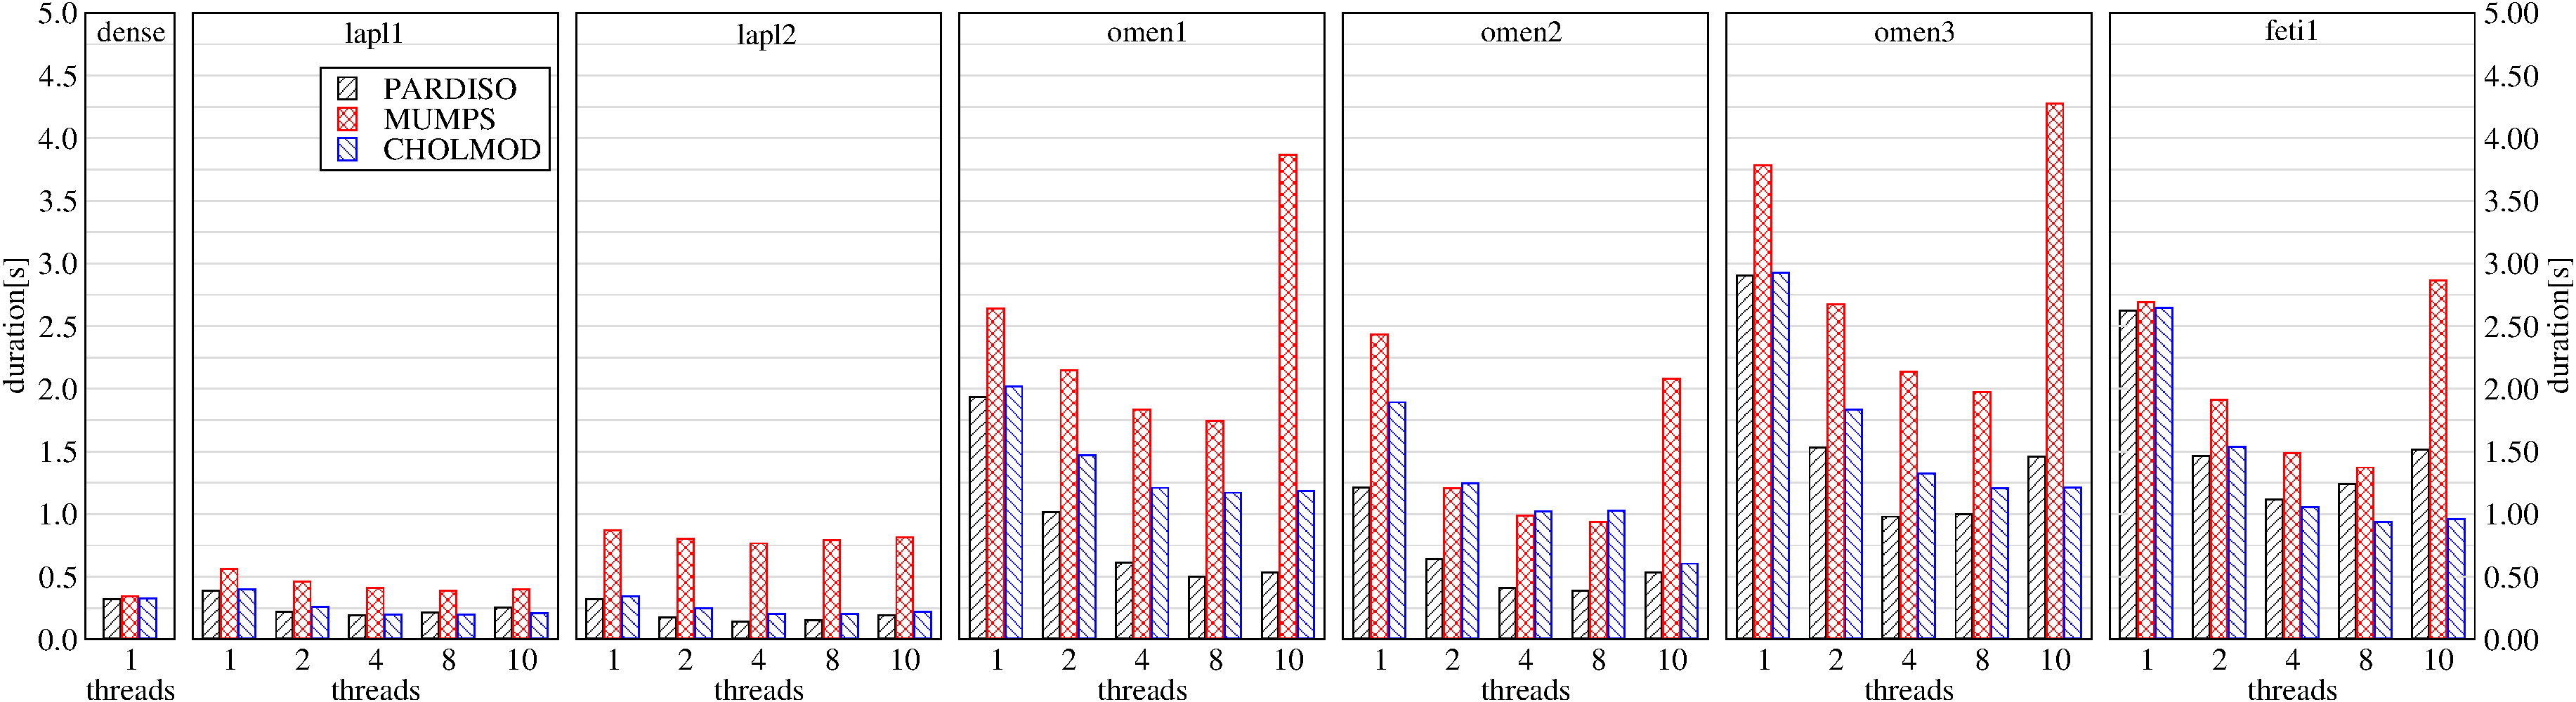
\includegraphics[width=\textwidth,clip=true]{images/SolverComparison}
   \caption{Duration of forward/backward substitution for the dense, lapl1, and lapl2 matrices for different sparse direct solvers on the IVB system.}
  \label{fig:solvers}
\end{figure}

In this chapter, we will mainly analyze the data transfer between the different cache levels and the FLOPs performed during the sparse triangular solve phase. The results of this analysis are used as input for our performance model. Therefore, we mostly inspect the different instantiations of the loops resulting from Algorithms~\ref{alg:algo:fw} and \ref{alg:algo:bw} on page \pageref{alg:algo:fw} and \pageref{alg:algo:bw}. We only consider the innermost loops because all the arithmetics are performed here. Our assumption is that the instructions regarding control variables of the loops are negligible, hence we do not them into account.
%Here, we only consider the innermost loops and do not
%distinguish between updates of~\vr{} or temporary arrays~\vtemp{}.

\section{Algorithm and data structures of sparse triangular solve}
% \section{Algorithm and Data Structures of the Forward/Backward Substitution}

\label{sec:algo}

Let $A$ be an $N \times N$ matrix and $x$ and $b$ be vectors of size $N$.
The linear system $A x = b$ is solved via $LDL^T$ decomposition by factorizing $A$
into a lower diagonal matrix $L$ and a diagonal matrix $D$ 
such
that $A =
LDL^T$.
The system is then solved in three steps. First,
$
  \label{eq:fw}
  Ly=b
$
is solved via forward substitution. This is followed by a diagonal solve
$
  \label{eq:dg}
  Dz=y
$
and, afterwards, the resulting $z$ vector is used to solve for the solution vector
%
$
  \label{eq:bw}
  L^Tx=z
$
% 
% via backward substitution. In sparse solver packages, such as, e.g.,
% PARDISO~\cite{schenk-2004}, 
via backward substitution. In 
PARDISO, 
the forward substitution is performed columnwise, starting with the
first column.
%mw first column, as depicted in Fig.~\ref{algo:triangular}~(a).
The data dependencies here allow us to store vectors $y$, $z$, $b$, and $x$ in
only one vector $r$. 

%\begin{figure}[t]
%  \centering
%    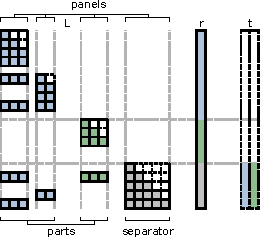
\includegraphics[width=0.55\linewidth,clip=true]{images/parts-panels-separator}
%  \caption{Sparse matrix data structures in PARDISO. Adjacent columns of $L$ exhibiting the same
%structure form panels also known as supernodes.
%Groups of panels which touch independent elements of the right-hand side $r$ are
%parts. The last part in the lower triangular matrix $L$ is called the separator.}
%  \label{fig:algo:ds}
%\end{figure}

The sparse matrix is stored in a PARDISO specific format shown in
Figure~\ref{fig:algo:ds}.
Adjacent columns exhibiting the same row sparsity structure form a
\textit{panel}, also known as a \textit{supernode}.
A panel's column count is called the \textit{panel size} $\panelsize$.
The columns of a panel are stored consecutively in memory excluding the zero
entries. 
Note that columns of panels are padded in the front with zeros so they get the 
same length as the first column inside their panel. 
The padding is of utmost importance for the PARDISO solver to use Level-2/3
BLAS and LAPACK functionalities. Please see~\cite{Bollhofer2020} for more
details.
Furthermore, panels are stored consecutively in the array \vlnz{}.
Row and column information is now stored in accompanying arrays.
%2 The \texttt{xsuper} array stores for each panel the index of its first column. 
%Also note that here column indices are the running count of nonzero columns.
Column indices are used as indices into the array \vxlnz{} to look up the
start of
the column in the array \vlnz{} which contains the numerical values of the factor $L$.
%2Panel~$p$ starts then in \vlnz{} at \vxlnz\texttt{[xsuper[p]]}.
To determine the row index of a column's element array \vindx{} is
used, which holds the row indices for each panel.
%2 The start of a panel inside \vindx{} is found via \vxindx{} array.
%2 The first row index of panel~$p$ is \vindx\texttt{[\vxindx[p]]}.

%2 For serial execution this information is enough. 
%2 However, during parallel forward/backward substitution concurrent updates to
%2 the same entry of \vr{} must be avoided.
For parallel execution concurrent updates to the same entry of \vr{} must be
avoided.
The \textit{parts} structure contains the start (and end) indices of the panels
which can be updated independently as they do not touch the same entries of $r$.
Two parts, colored blue and green, are shown in Figure~\ref{fig:algo:ds}.
The last part in the bottom right corner of $L$ is special and is called the 
\textit{separator} and is colored gray.
%
Parts which would touch entries of \vr{} in the range of the separator perform 
their updates into separate temporary arrays \vtemp{}.
Before the separator is then serially updated, the results of the temporary
arrays are gathered back into \vr{}. 
The backward substitution works the same, just reversed, and
updates to different temporary arrays are not required.
Figure \ref{fig:ecm-parallel-model} shows a possible execution of forward solve. The nested dissection reordering assigns to every partition about the same number of columns. However, panels in different partitions can have different size (number of columns). Then different threads execute differently unrolled code, as can be seen on the left side of Figure \ref{fig:ecm-parallel-model}. For easier modeling we assume the execution of the unrollings is sorted and evenly distributed over cores, as shows the right side of Figure \ref{fig:ecm-parallel-model}.

\begin{figure}[t]
  \centering
  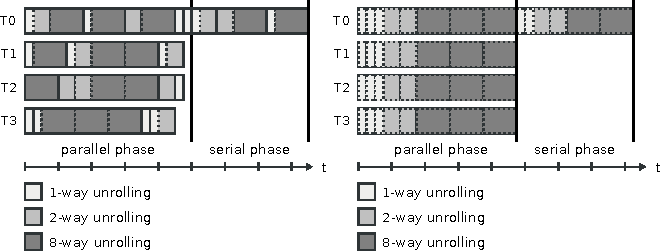
\includegraphics[width=0.9\textwidth,clip=true]{images/ecm-parallel-model}
   \caption{Possible real execution of forward solve. In the parallel phase cores can execute differently unrolled loops at the same time. For easier modeling the execution of the unrollings is sorted and evenly distributed over all cores.}
  \label{fig:ecm-parallel-model}%
\end{figure}

%\begin{algorithm}[t]
%  \begin{algorithmic}[1]
%    \Procedure{Sparse Forward Substitution}{}
%      \For{part in parts} \Comment{parallel execution}
%        \For{panel p in part}
%          \For{\textcolor{blue}{column $j$ in panel p}} \Comment{unroll} \label{alg:fw:1}
%            \State i = \nxindx{}[p] + offset
%
%            \For{k = \nxlnz[j] + offset; k < sep; ++k}\label{algo:fw:rloop}
%                \State row = \nindx[i++]
%                \State \nr[row] - =  \nr[j] \nlnz[k] \Comment{indexed DAXPY}
%            \EndFor\label{algo:fw:rloop:end}
%            \For{k = sep + 1; k < \nxlnz[j+1]; ++k}\label{algo:fw:seploop}
%                \State row = \nindx[i++]
%                \State \ntemp[row,p] -=  \nr[j] \nlnz[k] \Comment{indexed DAXPY}
%            \EndFor\label{algo:fw:seploop:end}
%          \EndFor
%        \EndFor
%      \EndFor
%
%      \State
%      \State r[i] = r[i] - sum(\ntemp[i,:])  \Comment{gather temporary arrays}
%      \State
%
%      \For{panel p in separator} \Comment{serial execution}
%        \For{\textcolor{blue}{column $j$ in panel p}} \Comment{unroll}\label{alg:fw:2}
%            \State i = \nxindx[p] + offset
%
%            \For{k = \nxlnz[j] + offset; k < \nxlnz[j+1]; ++k}\label{alg:fw:3}
%                \State row = \nindx[i++]
%                \State \nr[row] -=  \nr[j] \nlnz[k] \Comment{indexed DAXPY}
%            \EndFor
%        \EndFor
%      \EndFor
%    \EndProcedure
%  \end{algorithmic}
%  \caption{Forward substitution in PARDISO. Note that in the case of serial
%execution, separated updates to temporary arrays in lines
%\ref{algo:fw:seploop}--\ref{algo:fw:seploop:end} are not necessary
%and can be handled via the loop in lines
%\ref{algo:fw:rloop}--\ref{algo:fw:rloop:end}.}
%  \label{alg:algo:fw}
%\end{algorithm}
%
%\begin{algorithm}[tp]
%   \begin{algorithmic}[1]
%     \Procedure{Sparse Backward Substitution}{}
%       \For{panel $p$ in sep. rev.} \Comment{serial execution}
%         \For{\textcolor{blue}{col. $j$ in panel $p$ rev.}} \Comment{unroll}\label{alg:bw:1}
%            \State i = \nxindx[p] + offset
%
%            \For{k = \nxlnz[j] + offset; k < \nxlnz[j+1]; ++k}\label{alg:bw:3}
%                \State row = \nindx[i++]
%                \State \nr[j] -= \nr[row] \nlnz[k] \Comment{indexed DAXPY}
%            \EndFor
%
%            \State offset = offset - 1
%          \EndFor
%        \EndFor
%
%        \State
%
%        \For{part in parts} \Comment{parallel execution}
%          \For{panel $p$ in part rev.}
%            \For{\textcolor{blue}{col. $j$ in panel $p$ rev.}} \Comment{unroll}\label{alg:bw:2}
%
%              \State i = \nxindx[p] + offset
%
%              \For{k = \nxlnz[j] + offset; k < \nxlnz[j+1]; ++k}
%                \State row = \nindx[i++]
%                \State \nr[j] -=  \nr[row] \nlnz[k] \Comment{indexed DAXPY}
%              \EndFor
%
%              \State offset = offset - 1
%
%            \EndFor
%          \EndFor
%        \EndFor
%        \EndProcedure
%   \end{algorithmic}
%   \caption{Backward substitution in PARDISO. Separator (sep.), parts, and
%panels are iterated over in reversed (rev.) order.}
%   \label{alg:algo:bw}
%\end{algorithm}


% The complete forward backward substitution is listed in
% algorithm~\ref{alg:algo:fw} and~\ref{alg:algo:bw}, respectively.
% If no parallel execution is required then panels are updated successively in
% serial and during forward substitution updates to temporary arrays are not
% necessary.
The complete forward substitution is listed in Algorithm~\ref{alg:algo:fw}.
If no parallel execution is required then panels are updated successively in
serial, and during forward substitution, updates to temporary arrays are not
necessary.
Please note that through the dense storage of panels, indirect accesses to \vr{}
are required, resulting in an ``indexed DAXPY''-like operation, which prohibits a
straightforward vectorization.
% For performance reasons (discussed later in section~\ref{sec:pam}) the loops over the
% columns (blue text) in algorithms~\ref{alg:algo:fw} and~\ref{alg:algo:bw} are $1$-, $2$-,
% and $8$-way unrolled.
For performance reasons (discussed in Section~\ref{sec:pm:dt:wu}) the
loops over the columns (blue text) in Algorithm~\ref{alg:algo:fw} are $1$-,
$2$-, and $8$-way unrolled.
%\mycomment{OR: Blau wird im Druck nicht gut sichtbar sein. Ist uns das egal,
%weil wir sowieso nur vom PDF ausgehen? MW: ja davon wuerde ich ausgehen.}
The algorithm for the backward substitution in Algorithm~\ref{alg:algo:bw} 
looks nearly the same, except that
the serial part is executed first, which is then followed by the parallel section.
%

Parallel handling of the separator during the forward and backward
substitution is in principle possible.
Hereby the loops over the rows in line~\ref{alg:fw:3} of Algorithm~\ref{alg:algo:fw}
and line~\ref{alg:bw:3} of Algorithm~\ref{alg:algo:bw} would be parallelized.
However, typically the number of rows for sparse problems is too small to
benefit from this optimization and at worst it could introduce significant
overhead.

\section{Performance analysis of sparse triangular solve}
%\section{Analysis of the Forward/Backward Substitution} 
\label{sec:sds}

% \mycomment{OR: Werden die Daten analysiert oder ihr Transfer? MW: der Transfer
% natürlich :)}
%In this section, we analyze the data transfer between the different cache levels
%and the FLOPs performed during  the
%sparse triangular solve phase.
%%\sout{\OR the forward/backward substitution.}
%% \mycomment{OR: Fehlender Bezug durch ``which''. MW: OK}
%The results are used as input for our performance model
%to be
%established in the next section.
%%
%Therefore, we inspect the different instantiations of the loops resulting from
%Algorithm~\ref{alg:algo:fw} and~\ref{alg:algo:bw}.
%% \mycomment{``Hereby'' heisst ``hierdurch'', nicht ``hierbei''}
%Here, we only consider the innermost loops and do not
%distinguish between updates of~\vr{} or temporary arrays~\vtemp{}.

All entries %\sout{coefficients} 
of the matrix $L$
% \mycomment{OR: Bezeichnung ``coefficients'' hier gut? MW: entries? OR: OK.}
are stored as double-precision floating point
numbers in the vector \vlnz{}, consuming $8$\,B (byte) each.
Elements of the vector \vxlnz{} (column start indices in the vector \vlnz{}) and vector \vxindx{} (start
indices of row indices for each panel) are stored as $8$\,B integers,
whereas for the entries of the vector \vindx{} (row indices for each panel) $4$\,B integers
are used.
\enlargethispage*{\baselineskip}

\subsection{Data transfers and FLOPs without unrolling}
\label{sec:pm:dt}
\label{sec:pm:dt:wou}

% \begin{figure}[t]
%   \centering
%  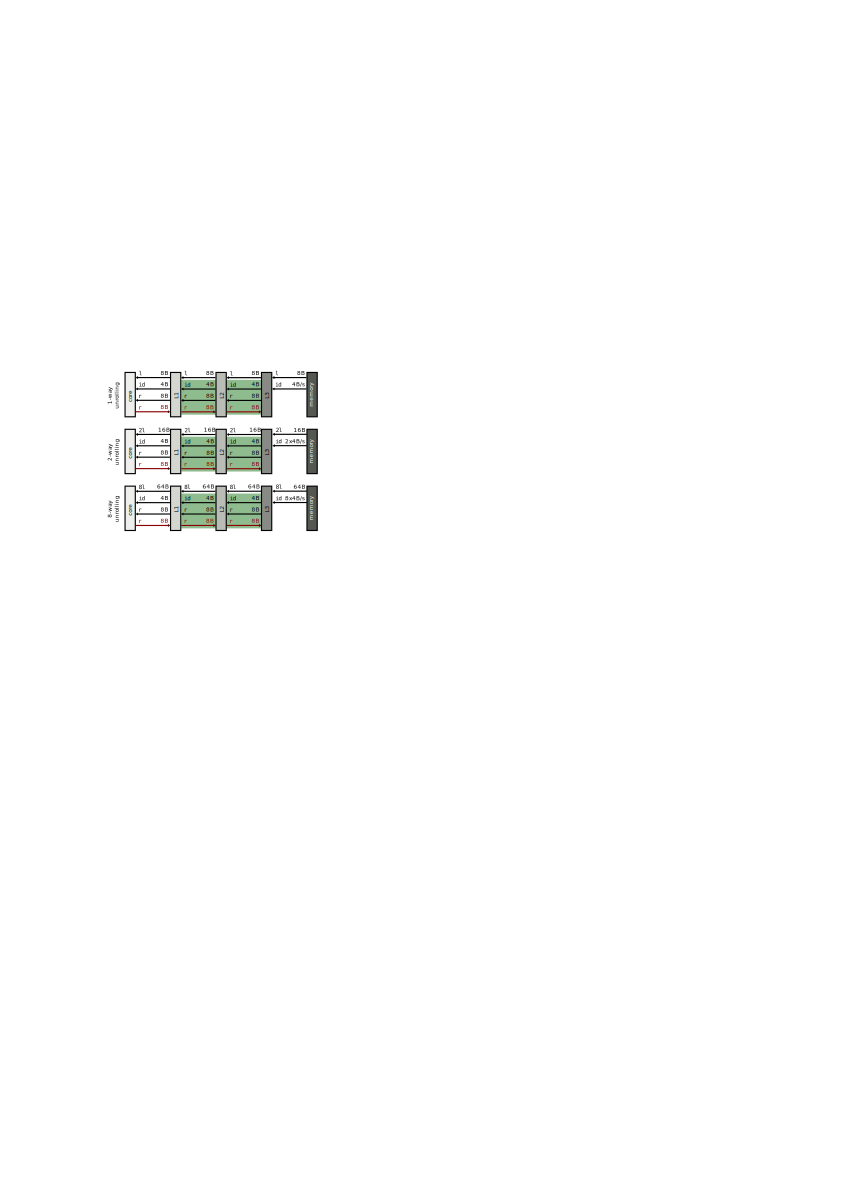
\includegraphics[width=0.43\textwidth,clip=true]{images/ecm-datatransfers}
%   \caption{Data transfers for one iteration of the forward
%     (including red text and arrows) and backward (without red text and arrows)
%     substitution when $1$-, $2$-, or $8$-way column unrolling is applied.
%     Thereby $1$, $2$, or $8$ nonzero elements of \vlnz{} are processed,
%     respectively.
% %    Loading of \vindx{} from memory (blue boxes) is only included in the model 
% %    if the panel size $s \le 8$.
% % From which cache level \vr{} is reused (green boxes) depends on the size of the
% % active part. If the active part is large it must be reloaded from
% % L3 cache. With decreasing size it can fit into L2 or even L1 cache.
% % This holds also true for \vindx{}, but additionally depends on the panel size.
%   }
%   \label{fig:ecm:data}
% \end{figure}
% 

In the most simple case no unrolling is applied and the innermost loop of
forward substitution from Algorithm~\ref{alg:algo:fw} looks like
% \mycomment{OR: sollte der Alg.~\ref{alg:algo:fw} nicht
% eine Float-Umgebung bekommen? MW: algorithm ist doch eine float-Umgebung.
% OR: Habe mich vertan.
% }
%
\begin{algorithmic}[1]
  \setcounter{ALG@line}{20}
  \For{k = \nxlnz[j] + offset; k < \nxlnz[j+1]; ++k}
      \State row = \nindx[i++]
      \State \nr[row] -= \nr[j] \nlnz[k]
  \EndFor
\end{algorithmic}%
%\vspace{-\baselineskip}
\noindent%
%
As the loops from lines $6$--$9$ and $10$--$13$ are in principle identical to
the loops in lines $21$--$24$, we only discuss the latter.
%
During each iteration one nonzero is processed, two FLOPs are performed,
namely, a multiplication and an addition, and the following elements get
loaded and stored: loaded: \vindx{} ($4$~\,B), \vr{} ($8$~\,B), \vlnz{}
($8$~\,B); stored: \vr{} ($8$~\,B).

How much data are transferred inside the cache hierarchy depends on the size of
the caches, their replacement strategies, the size of \vr{}, the average panel
size, as well as the structure of the panels, i.e.,\ which part of \vr{} is
accessed.
Here we assume \vr{} is small enough to be kept at least in last level cache
(LLC) and temporal locality ensures it is not evicted.
%
Row indices in \vindx{} for a panel are loaded from memory for the panel's first
column and then are reused during each iteration over the panel's remaining
columns from the LLC in the worst case.
With panel size $\panelsize=1$, for each element of \vlnz{} one row index is
transferred and no reuse is possible.
In general reuse is only possible, starting with a panel's second column for
panel sizes $\panelsize \ge 2$.
%
Coefficients of \vlnz{} are always streamed in from memory, as they are
used only once and the array \vlnz{} is typically too large to be kept in LLC.
Figure~\ref{fig:ecm:data-fw} visualizes the transfers assuming three cache levels
and \vr{} is cached in LLC.
While iterating over panels and columns, the number of column elements
decreases as $L$ is a lower triangular matrix.
Thereby the number of used elements from \vr{} also decreases, which we call the
active part of \vr{}.
At some point the active part can be completely kept in the L2 or even the L1 cache.
This also holds true for \vindx{}, except when a new panel starts, then
the panel's row indices must first be loaded from memory.
With Intel L2 cache 256\,kB and L1 cache 32\,kB, a maximum of about 13000 and 1600 elements of \vr{}, \vindx{}, and \vlnz{} could fit into the L2 and L1 caches, respectively. However, due to the associativity and replacement strategy of the cache and the need to store other data, it is reasonable to expect only half of the size can be used. We can expect if the active part of \vr{} is less than about 6000 elements, it can be kept in the L2 cache, and if it is less than about 800 elements it fits into the L1 cache.
\clearpage

\begin{figure}[t]
  \centering%
%  \includegraphics[width=0.3\textwidth,clip=true]{images/ecm-datatransfers-1}
%  \includegraphics[width=0.3\textwidth,clip=true]{images/ecm-datatransfers-2}
%  \includegraphics[width=0.3\textwidth,clip=true]{images/ecm-datatransfers-8}
  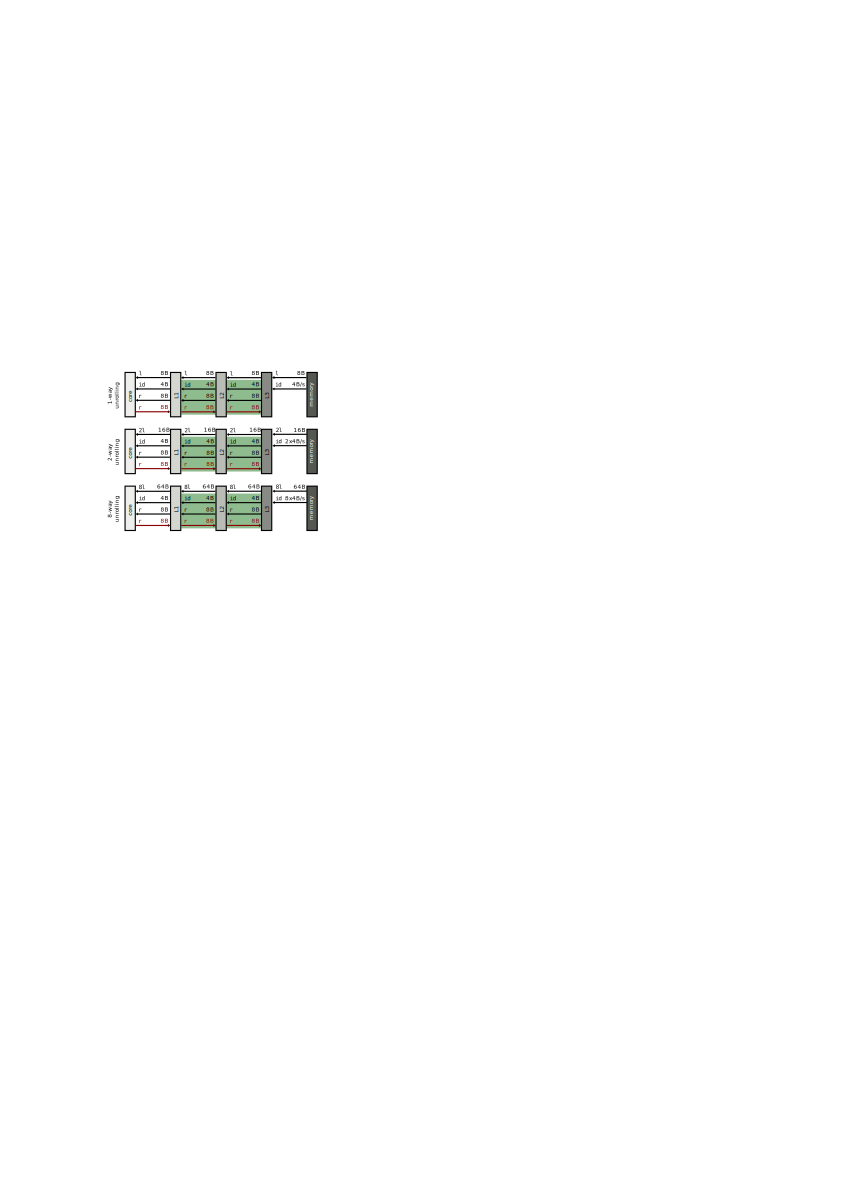
\includegraphics[width=0.75\linewidth,clip=true]{images/ecm-datatransfers-fw}
  \caption{Data transfers for one iteration of the forward
    substitution when \protect\linebreak $1$-, $2$-, or $8$-way column unrolling is applied
    for a panel with panel size $s$.
    Thereby $1$, $2$, or $8$ nonzero elements of \vlnz{} are processed,
    respectively.
%    Loading of \vindx{} from memory (blue boxes) is only included in the model
%    if the panel size $s \le 8$.
% From which cache level \vr{} is reused (green boxes) depends on the size of the
% active part. If the active part is large it must be reloaded from
% L3 cache. With decreasing size it can fit into L2 or even L1 cache.
% This holds also true for \vindx{}, but additionally depends on the panel size.
  }
  \label{fig:ecm:data-fw}
\end{figure}

%
%1 The active part of \vr{} can be kept inside a certain cache size $c_s$, when
%1 concurrently also one column of \vlnz{} and the active part of \vindx{} fit into
%1 this cache level.
%1 Let $n_j$ the length of column $j$. 
%1 If $L$ is dense, like for the dense matrix, then if $n_j \le c_s/(8\,\text{B} + 8\,\text{B} +
%1 4\,\text{B})$ holds true all active parts fit into the cache.
%1 %
%1 If instead in the worst case $L$ is sparse so that only one element out of a cache
%1 line from \vr{} is accessed
%1 then $n_j \le c_s/(8\,\text{B} + 64\,\text{B} + 4\,\text{B})$ is required.
%1 %
%1 Note that already when the active part of \vr{} slightly exceeds the determined
%1 limits already partial caching in the same cache level takes place\footnote{If
%1 we
%1 load a vector which exceeds the cache size several times it must be completely
%1 reloaded during each iteration. 
%1 However, if the cache utilizes a least recently used policy and the vector's
%1 size is in the range of the cache size $c_s$ and $c_s + w_s$, where $w_s$
%1 denotes the way size of the cache, then still parts of the vector are held in
%1 the cache and need not to be reloaded.
%1 The way size of a cache is defined as the product of the cache's number of sets
%1 and the cache line size.}.

The innermost loop of the backward substitution from
Algorithm~\ref{alg:algo:bw} is %looks like
% The innermost loop from lines $5$--$9$ is the same as the one from lines
% $17$--$20$ of the backward
% substitution from Algorithm~\ref{alg:algo:bw}, which we only discuss the former,
% which looks like 
%
\begin{algorithmic}[1]
\setcounter{ALG@line}{4}
  \For{k = \nxlnz[j] + offset; k < \nxlnz[j+1]; ++k}
    \State row = \nindx[i++]
    \State \nr[j] = \nr[j] - \nr[row] \nlnz[k]
  \EndFor
\end{algorithmic}%
%\vspace{-\baselineskip}
\noindent%
%
As this loop from lines $5$--$8$ is the same as the one from lines $16$--$19$,
all following statements hold true for both. 
%
As with forward substitution one nonzero is processed, two FLOPs are performed,
but only loads occur: \vindx{} ($4$~\,B), \vr{} ($8$~\,B), and \vlnz{} ($8$~\,B).
Note that $j$ is unchanged in the innermost loop, hence $\nr[j]$ always refers
to the same element and is not considered for the data transfer analysis.
%
Figure~\ref{fig:ecm:data-bw} displays the data transfers occurring for one
nonzero update if \vr{} is cached in L3 cache.

\begin{figure}[t]
  \centering%
%  \includegraphics[width=0.3\textwidth,clip=true]{images/ecm-datatransfers-1}
%  \includegraphics[width=0.3\textwidth,clip=true]{images/ecm-datatransfers-2}
%  \includegraphics[width=0.3\textwidth,clip=true]{images/ecm-datatransfers-8}
  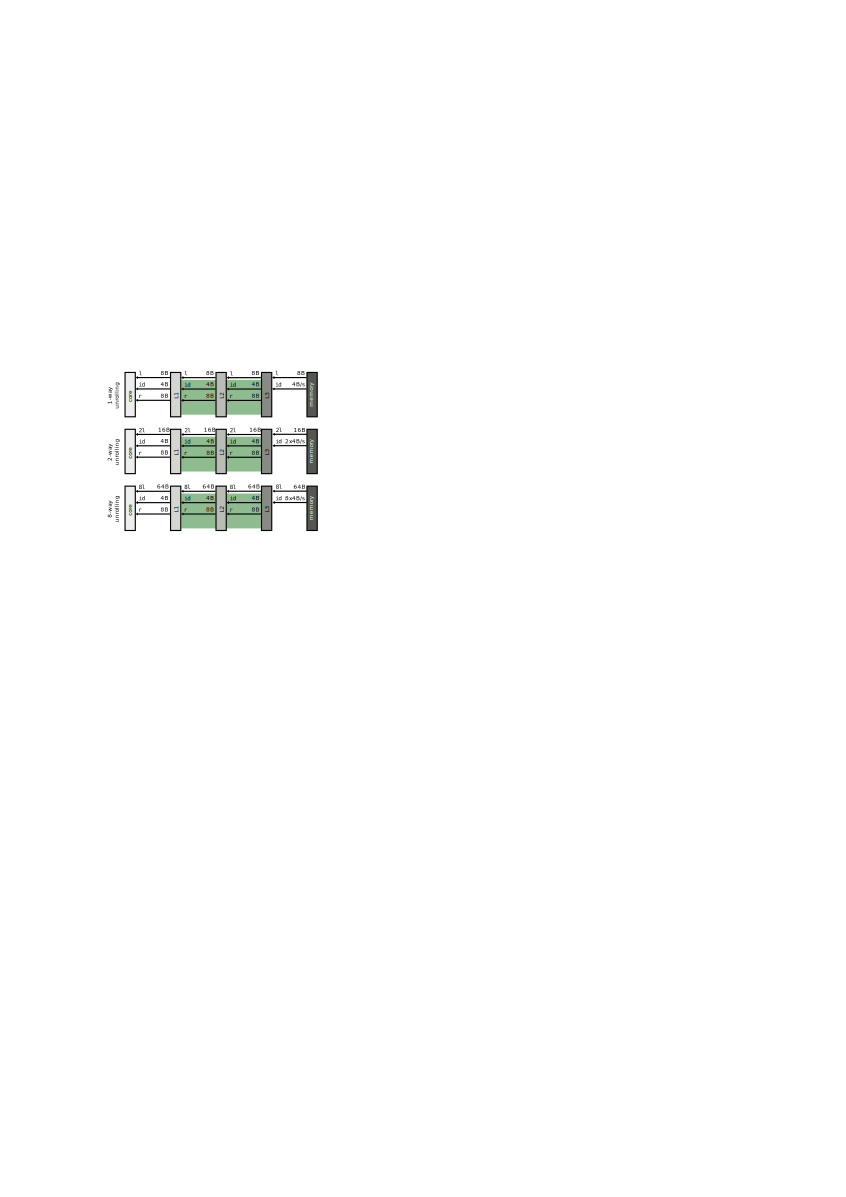
\includegraphics[width=0.75\linewidth,clip=true]{images/ecm-datatransfers-bw}
  \caption{Data transfers for one iteration of the backward
    substitution when $1$-, $2$-, or $8$-way column unrolling is applied
    for a panel with panel size $s$.
    Thereby $1$, $2$, or $8$ nonzero elements of \vlnz{} are processed,
    respectively.
%    Loading of \vindx{} from memory (blue boxes) is only included in the model
%    if the panel size $s \le 8$.
% From which cache level \vr{} is reused (green boxes) depends on the size of the
% active part. If the active part is large it must be reloaded from
% L3 cache. With decreasing size it can fit into L2 or even L1 cache.
% This holds also true for \vindx{}, but additionally depends on the panel size.
  }
  \label{fig:ecm:data-bw}
\end{figure}

\subsection{Data transfers and FLOPs with unrolling}
\label{sec:pm:dt:wu}

%
As noted in Section~\ref{sec:algo} it is beneficial to handle several columns
at once.
%\sout{In PARDISO loops over columns \uwave{are additionally to no unrolling manually $2$- and $8$-times unrolled and used when a panel contains more than one column.}}
For this purpose PARDISO has additionally 2- and 8-way manually unrolled
loops over columns.  These are used when a panel contains more than one column.
With an unrolling factor of two the innermost loop for forward substitution becomes
%
\begin{algorithmic}[1]
  \State nj = nonzero column length
  \For{k = \nxlnz[j] + offset; k < \nxlnz[j+1]; \textcolor{blue}{k += 2}}
      \State row = \nindx[i++]
      \State \nr[row] = \nr[row] - \nr[j] \nlnz[k] \textcolor{blue}{- \nr[j+1] \nlnz[k+nj]}
  \EndFor
\end{algorithmic}%
%\vspace{-\baselineskip}
\noindent%
%
%\sout{\uwave{In contrast to no unrolling per iteration two nonzeros are processed.}}
Instead of processing only one nonzero the 2-way unrolling handles two
nonzeros per iteration.
Hence, four FLOPs are performed and two entries of \vlnz{} are loaded.
Hereby the corresponding element of \vr{} only needs to be loaded once instead of
twice, when processing two elements of \vlnz{}.
All other transfers stay unchanged.
%
In general with a $u$-way unrolling during each iteration, $2 \times u$\,FLOPs
are executed and $u \times 8\,\text{B} + 20\,\text{B}$ are transferred.

Unrolling of the backward substitution loop results in the following code for a
$2$-way unrolling:
%mw2018-06-07: \mycomment{ML: Bin fuer konsistenz: two-way und two-time
%mw2018-06-07: unrolling oder 2-way und 2-time unrolling. MW: OK}
%
\begin{algorithmic}[1]
  \State nj = nonzero column length
  \For{k = \nxlnz[j] + offset; k < \nxlnz[j+1]; \textcolor{blue}{k += 2}}
      \State row = \nindx[i++]
      \State \nr[j]   = \nr[j] - \nlnz[k] \nr[row]
      \State \textcolor{blue}{\nr[j+1]   = \nr[j+1] - \nlnz[k+nj] \nr[row]}
  \EndFor
\end{algorithmic}%
%\vspace{-\baselineskip}
\noindent%
%
Also here four FLOPs per iteration are performed, two entries of \vlnz{} are
loaded and the corresponding element of \vr{} is loaded only once.
%
For a $u$-way unrolling, $2 \times u$\,FLOPs and $u \times 12\,\text{B} +
8\,\text{B}$ are loaded.

As already noted, we assume \vr{} and a panel's current row indices from
\vindx{} are at least cached in LLC or higher cache levels.
%
Unrolling, hereby, only saves transfers inside the cache hierarchy.
The bytes transferred between memory and LLC are left unaffected and depend only
on the panel size.
With larger panel sizes in total, fewer
row indices \vindx{} are needed for the
whole matrix.

\section[Application of modified Berkeley roofline model]{Application of modified Berkeley roofline model on sparse triangular solve}
\label{sec:mrm}

% \begin{table}[tp]
%   \small
%   \centering
%   \begin{tabular}{llcRRRccRRR}
%   \hline
%   \multirow{2}{*}{u}&& \multicolumn{4}{c}{forward}  && \multicolumn{4}{c}{backward} \\
%   \cline{3-6} \cline{8-11}
%    && \mcco{L1} & \mcco{L2} & \mcco{L3} & \mcco{mem} && \mcco{L1} & \mcco{L2} & \mcco{L3} & \mcco{mem}\\
%   \hline
%   1 && 14   & 4 - 14  &  4 - 14  & 4 - 6    && 10   & 4 -  10 & 4 -  10 & 4  - 6 \\ 
%   2 &&  9   & 4 -  9  &  4 -  9  & 4 - 5    &&  7   & 4 -   7 & 4 -   7 & 4  - 5 \\
%   8 && 5.25 & 4 - 5.25&  4 - 5.25& 4 - 4.25 && 4.75 & 4 -  4.75&4 - 4.75& 4  - 4.25 \\
%   \hline
%   \end{tabular}
%   \caption{Code balance $B_c$ [B/F] of forward/backward substitution for
% different unrollings (u) when
% data is fetched from the corresponding level inside the memory hierarchy. Values
% depend on actual panel size $s$ and possible cache reuse.}
%   \label{tab:mrm:bc}
% \end{table}

%xx \begin{table*}[!t]
%xx   \caption{Details of Evaluated Hardware Systems.
%xx % ISA Lists the Latest Extension Supported by the Processor. 
%xx % Read Memory Bandwidth, Floating Point Instructions per Cycle (ADD+MULL and
%xx % FMA Instructions), and Machine Balance is Reported for Scalar Execution.
%xx KNL's Bandwidth Numbers are for DDR Memory.}
%xx % ECM: 2 cy L1/L2 bei HSW/BDW entgegen der Doku 
%xx % STREAM:
%xx % read = summation
%xx % KNL: no-nt, prefetch not explicitly disabled
%xx % ZEN: no-nt, AVX2, only even cores
%xx % HSW2: no-nt, avx2
%xx % HSW: no-nt, avx2
%xx % IVB: no-nt, 
%xx   \label{tab:hw}
%xx   \footnotesize
%xx  \centering
%xx %\resizebox{\textwidth}{!}{%
%xx  \begin{tabular}{p{1.9cm}llrrrrrrrrr}
%xx     \hline
%xx     name      & &  & IVB         & HSW-D      & HSW-S           & BDW           & SKX         & KNL           & ZEN-D        &  ZEN-S         \\
%xx     \hline                                                      
%xx     \multirow{3}{\linewidth}{processor name} & &  & Intel& Intel & Intel & Intel & Intel & Intel & AMD &  AMD \\
%xx       & &  & Xeon  & Xeon & Xeon      & Xeon    & Xeon  & Xeon    &
%xx ~~Ryzen 7   &  ~~EPYC      \\
%xx               & &  &\scriptsize  E5-2660 v2 &\scriptsize  E3-1240 v3
%xx &\scriptsize  E5-2695 v3      &\scriptsize  E5-2630 v4    &\scriptsize  Gold
%xx 6148   &\scriptsize  Phi 7210      &\scriptsize  1700X      &\scriptsize
%xx 745           \\
%xx %     processor & &  & Intel Xeon  & Intel Xeon & Intel Xeon      & Intel Xeon    & Intel Xeon  & Intel Xeon    & AMD Ryzen    &  AMD EPYC      \\
%xx %     name      & &  &  E5-2660 v2 & E3-1240 v3 & E5-2695 v3      & E5-2630 v4    & Gold 6148   & Phi 7210      & 7 1700X      &  745           \\
%xx     \hline                                                      
%xx     micro     & &  & Ivy Bridge  & Haswell    & Haswell         & Broadwell
%xx & Skylake     & ~Knigths       & Zen          &  Zen           \\
%xx     arch.     & &  &             &            &                 &               &             & Landing       & \\
%xx     \hline                                                    
%xx     freq    & [GHz] & & 2.2      & 3.4        & 2.3             & 2.2           & 2.4         & $\approx$ 1.3 & 3.4          &  2.3           \\
%xx     cores   &       & & 10       & 4          & 2 $\times$ 7    & 10            & 20          & 64            &   8          &  24            \\
%xx     ISA     &       & & AVX      & AVX2       & AVX2            & AVX2          & AVX-512     & AVX-512       & AVX2         &  AVX2          \\
%xx %    sockets &       & 2        & 1          & 2               & 2             & 2           & 1             & 1            &  & 1 \\
%xx %    \mltwo{NUMA LDs}& 2        & 1          & 2 $\times$ 2    & 2 $\times$ 2  & 2           & 1             & 1            &  & 1 \\
%xx     \mltwo{NUMA LDs} & & 1       & 1          & 2               & 1             & 1           & 1             & 1            & 4              \\
%xx     \hline                                                    
%xx     L1 & [KiB]     &  &  32      & 32         & 32              & 32            & 32          & 32            & 32           &  32            \\
%xx     L2 & [KiB]     &  &  256     & 256        & 256             & 256           & 1024        & 1024          & 512          &  512           \\
%xx     L3 & [MiB]     &  &  25      & 8          & 2 $\times$ 17.5 & 25            & 28          & -             & 2 $\times$ 8 &  8 $\times$ 8 \\ 
%xx     \hline
%xx %    copy bw. & [GB/s] & 41.2   & 26.6            & 22.6       & 31.3 & ?? &  75.9 & 30.2 & 212 \\ % complete socket/cod
%xx %    read bw. & [GB/s] & 44.3   & 30.9            & 23.6       & 33.7 & ?? &  74.2 & 32.5 & 231 \\ % complete socket/cod
%xx     \mlfour{scalar read bw.}   &     &          &  \\
%xx     ~1 core  & [GB/s]  &&  9.5 & 16.6 & 12.1 & 11.5 &  14.5 &  8.5 & 19.3 & 19.3  \\
%xx     ~NUMA LD & [GB/s]  && 44.4 & 22.7 & 31.2 & 56.3 & 108.0 & 75.2 & 33.7 & 37.6  \\
%xx     \hline
%xx     \mlfour{scalar ADD+MUL/FMA} &&& \\
%xx     ~1 core  & [F/cy] &&  2 &  4 &  4 &  4 &  4 &   4 &  4 &  4 \\
%xx     ~NUMA LD & [F/cy] && 20 & 16 & 28 & 40 & 80 & 256 & 32 & 24 \\
%xx     \hline
%xx     \mlfour{scalar machine balance $B_m$} &  &         & \\
%xx     ~1 core  & [B/F] && 2.2 & 1.2 & 1.3 & 1.3 & 1.5 & 1.6 & 1.4 & 2.1 \\
%xx     ~NUMA LD & [B/F] && 1.0 & 0.4 & 0.5 & 0.6 & 0.6 & 0.2 & 0.3 & 0.7 \\
%xx     \hline
%xx \\[0.01em]
%xx   \end{tabular}
%xx %} % from https://tex.stackexchange.com/a/27105
%xx \end{table*}
%\parbox{.25\linewidth}{ 
%\begin{SCtable}[][t]

For our performance predictions of the sparse triangular solve, we apply the roofline model~(\cite{williams-2009}).
As mentioned before, the model takes into account the attainable memory bandwidth as well as
the
peak floating
point performance of the processor and 
%\uwave{%\sout{correlates}
relates these hardware capabilities %\sout{with}
to
the requirements of the code.
%}
%mw2018-06-07: \mycomment{OR: was heisst dieses? MW: besser? OR: Etwas. Aber inwiefern wird
%mw2018-06-07: eine Beziehung zu den Anforderungen hergestellt? MW: Die Code-Balance $B_c$ ist
%mw2018-06-07: die Anforderung des Codes und $B$ bzw.\ $P_\text{max}$ stammt von der Hardware.}
It can be written as
%
\be
  P = \min(P_\text{max}, B / B_c),
\ee
where $P_\text{max}$ denotes the attainable floating point performance, $B$ the
attainable memory bandwidth, and $B_c$ the code balance.

Here, $P_\text{max}$
depends already on the floating point characteristics of the code and the
processor and does not represent the peak floating point performance as it can
be obtained from a processor's data sheet. 
If a processor supports vectorized FMA instructions, but
only vectorized add or multiply instructions are used, then $P_\text{max}$ is
halved.
Using scalar instructions instead of the AVX vectorized counterparts reduces
$P_\text{max}$ further by a factor of four.
%
And, finally, if the floating point instruction mix does not equally utilize a
processors floating point units, $P_\text{max}$ is again reduced.
% \todo{This is a forward reference.}
For example, the Ivy Bridge (IVB) system (Section~\ref{sec:tb}, Table~\ref{tab:hw}) hosts an add and
multiply unit, but if only one type of floating point instruction is used, only
half of the theoretical floating
point performance can be attained. 
%
In our case the compiler uses 
scalar FMA instructions
for the core loops of the %\sout{forward/backward substitution} 
sparse triangular solve
for architectures
with AVX2 support and scalar \linebreak add/multiply instructions for
architectures without FMA support like IVB.

The attainable memory bandwidth $B$ is measured with a microbenchmark,
ideally resembling the application's memory access pattern. 
For the
sparse triangular solve,
%\sout{\OR the forward/backward substitution}
we use a read-only benchmark from the LIKWID tool suite (\cite{likwid-2010-arxiv}).
%
As the sparse triangular solve
%\sout{\OR the forward/backward substitution}
in PARDISO only uses scalar load instructions we also use them
for the microbenchmark. 

The \textit{code balance} $B_c$ is the ratio of bytes transferred to the
number of FLOPs performed in the code.
In the best case, when the panel size $\panelsize$ is large and the indices are
cached, during the forward~\eqref{eq:algo:fw:pardiso} and backward
substitutions~\eqref{eq:algo:bw:pardiso}, each nonzero of $L$ must be loaded once
and the loading of indices can be neglected,
respectively. 
Furthermore, the computation involves two FLOPs per nonzero.
As nonzeros are stored in double precision consuming $8$\,B, this results in a
best case code balance of $B_c = 8 / 2 \text{B/F} = 4 \text{B/F}$, where F
denotes FLOP.
%1 Table~\ref{tab:mrm:bc} lists the code balance for different unrollings and cache
%1 levels and uses the data transfer and FLOP counts from Sect.~\ref{sec:sds}.
Table~\ref{tab:mrm:bc} lists the code balance for different unrolling factors
when the factor $L$ must be fetched from memory and uses the data transfer and
FLOP counts from Section~\ref{sec:sds}.
In contrast, the \textit{machine balance} $B_m$ defines the ratio for the whole system
and uses the ratio of the attainable memory bandwidth $B$ to the maximum floating point
performance $P_\text{max}$.
% \todo{This is a forward reference.}
% \mycomment{OR: Tab. ist keine erlaubte Abkuerzung f\"ur Table. MW: stimmt}
This bandwidth is found in Table~\ref{tab:hw} for all systems.
%
If $B_c > B_m$ then the roofline model indicates 
that the code's performance is
limited by the memory bandwidth,
i.e., that the code is memory bound.
%1 This is the case for sparse direct solve for all unrollings, when data is
%1 located in L2, L3, or memory.
{This is the case for the sparse %\sout{direct} 
triangular solve 
phase %\sout{for} 
of all
%mw2018-06-07: \uwave{
unrolling factors,
%mw2018-06-07: }
when the factor $L$ is too large to be kept in cache and
completely located in memory.}
%mw2018-06-07: \mycomment{\OR was meint ``unrolling factor'' hier? \MW MW: Das ist der Faktor
%mw2018-06-07: für das ``loop unrolling''. Der Begriff wird vorher auch schon so verwendet,
%mw2018-06-07: daher haette ich den nicht nocheinmal erlaeutert.}

\begin{table}[t]
  \centering
   \begin{tabular}{ll|cm{0.8eM}cm{0.8eM}c|cm{0.8eM}cm{0.8eM}c}
  \hline
  Substitution && \multicolumn{5}{c|}{Forward} & \multicolumn{5}{c}{Backward} \\
  %\cline{3-5} \cline{7-9}
  \hline
     $u$    &     &  1   &  & 2    &  & 8        & 1     &  & 2   &  & 8  \\
     $B_c$  & [B/F]\, & \ $4-6$ & & $4-5$ & & $4-4.25$ \ & \ $4-6$ & & $4-5$ & & $4-4.25$ \ \\
  \hline
  \end{tabular}
  \caption{Code balance $B_c$ of forward/backward substitution for
unrolling factors $u$ when
the factor $L$ must be fetched from memory.
% the factor $L$ exceeds the LLC and must be fetched from memory.
Values depend on actual panel size $s$ and possible cache reuse.}
  \label{tab:mrm:bc}
\end{table}

To determine performance limits, we only consider the case when data reside in
memory.
Therefore the data transfers between the L3 cache and memory are relevant as shown
in Figures~\ref{fig:ecm:data-fw} and \ref{fig:ecm:data-bw}.
Only nonzero entries of $L$ with the corresponding panel indices are loaded. 
Their amount depends only on the structure of $L$ and is independent of the used
loop unrollings.
%
The roofline model for the memory bound case as a function of the number of
threads~$t$ can be formulated as
%
\be
  \label{eq:rm:simple}
  P^{A}(t)
  = \frac{
      \text{nnz} (L) \times 2 \frac { \text{FLOP}}{ \text{nz}}
    }{
     \frac{D_A(t)}{ B(t)} 
    } \quad \frac{\text{FLOP}}{s},
\ee
%
%\mycomment{OR: Genaugenommen sind Einheiten in eckigen Klammern veraltet;
%https://de.wikipedia.org/wiki/Einheitenzeichen MW: OK, die Einheiten in Klammern
%in den Tabellen sollten aber passen.
%OR: Es ist mir nicht so wichtig, es kann auch in eckige Klammern.
%}
where $\text{nnz}(L)$ denotes the number of nonzeros of the factor $L$ 
resulting from a factorization of $A$ for $t$ threads, 
$B(t)$ is the attainable memory bandwidth of the system utilizing $t$ threads, and 
$D_A(t)$ the data volume of nonzeros and indices making up $L$.
The only adjustment to the original model here is its dependency on the number
of threads. 
Choosing $t$ equal to the number of total cores yields the original roofline model.

To distinguish between the parallel phase, where the parts are handled,
and the serial part, where the separator is treated, we modify 
\eqref{eq:rm:simple}.
We use the following formula for the \textit{modified roofline model}: 
%
\be
  \label{eq:rm:mod}
  P^{A}_{\text{mod}}(t) 
  = \frac{
      \text{nnz} (L) \times 2 \frac { \text{FLOP}}{ \text{nz}}
    }{
     \frac{D_A^p(t) }{  B(t) } + \frac{ D_A^s(t) }{ B(1) }
    } \quad \frac{\text{FLOP}}{s},
\ee
%
where
$D_A^p(t)$ 
represents
the data volume of nonzeros and indices %\sout{\uwave{made up}} 
built up
% \mycomment{OR: ``made up''? Erfunden? MW: OK}
by the parallel parts, and $D_A^s(t)$ the data volume %\sout{\uwave{made up}}
built up by the nonzeros and
indices of the separator.
%
Please note that both data volumes $D_A^p(t)$ and $D_A^s(t)$ depend on
$A$ and the number of threads $t$.
%
The values for $D_A^p(t)$ and $D_A^s(t)$ are extracted from the factorized
matrices a priori to solve.

Please note that the accuracy of the roofline model predictions, especially for
single cores, as included in the modified model, can be inaccurate. 
%\mycomment{OR: Auf welches Ganzes bezieht sich ``part''? MW: Done.}
If the in-core execution time (excluding floating point operations) or the in-cache
traffic dominates the execution time, predictions become unreliable as this is not
covered by the roofline model.
In Chapter~\ref{sec:performance}, we use dedicated single core measurements to
validate that, in the case of the sparse triangular solve,
%\sout{\OR the forward/backward substitution,}
this approach is valid. 
%
However, this effect can be modeled in detail with the ECM
model (\cite{treibig-2010-ecm, hager-2012-ecm, stengel-2015}) and was already
studied for stencil kernels.


%-- \begin{table*}[!t]
%-- \parbox{.7\linewidth}{
%--   \caption{Details of Evaluated Hardware Systems.
%-- % ISA Lists the Latest Extension Supported by the Processor. 
%-- % Read Memory Bandwidth, Floating Point Instructions per Cycle (ADD+MULL and
%-- % FMA Instructions), and Machine Balance is Reported for Scalar Execution.
%-- KNL's Bandwidth Numbers are for DDR Memory.}
%-- % ECM: 2 cy L1/L2 bei HSW/BDW entgegen der Doku 
%-- % STREAM:
%-- % read = summation
%-- % KNL: no-nt, prefetch not explicitly disabled
%-- % ZEN: no-nt, AVX2, only even cores
%-- % HSW2: no-nt, avx2
%-- % HSW: no-nt, avx2
%-- % IVB: no-nt, 
%--   \label{tab:hw}
%--   \footnotesize
%--  \centering
%-- %\resizebox{\textwidth}{!}{%
%--  \begin{tabular}{p{1.9cm}llrrrrrrrrr}
%--     \hline
%--     name      & &  & IVB         & HSW-D      & HSW-S           & BDW           & SKX         & KNL           & ZEN-D        &  ZEN-S         \\
%--     \hline                                                      
%--     \multirow{3}{\linewidth}{processor name} & &  & Intel& Intel & Intel & Intel & Intel & Intel & AMD &  AMD \\
%--       & &  & Xeon  & Xeon & Xeon      & Xeon    & Xeon  & Xeon    &
%-- ~~Ryzen 7   &  ~~EPYC      \\
%--               & &  &\scriptsize  E5-2660 v2 &\scriptsize  E3-1240 v3
%-- &\scriptsize  E5-2695 v3      &\scriptsize  E5-2630 v4    &\scriptsize  Gold
%-- 6148   &\scriptsize  Phi 7210      &\scriptsize  1700X      &\scriptsize
%-- 745           \\
%-- %     processor & &  & Intel Xeon  & Intel Xeon & Intel Xeon      & Intel Xeon    & Intel Xeon  & Intel Xeon    & AMD Ryzen    &  AMD EPYC      \\
%-- %     name      & &  &  E5-2660 v2 & E3-1240 v3 & E5-2695 v3      & E5-2630 v4    & Gold 6148   & Phi 7210      & 7 1700X      &  745           \\
%--     \hline                                                      
%--     micro     & &  & Ivy Bridge  & Haswell    & Haswell         & Broadwell
%-- & Skylake     & ~Knigths       & Zen          &  Zen           \\
%--     arch.     & &  &             &            &                 &               &             & Landing       & \\
%--     \hline                                                    
%--     freq    & [GHz] & & 2.2      & 3.4        & 2.3             & 2.2           & 2.4         & $\approx$ 1.3 & 3.4          &  2.3           \\
%--     cores   &       & & 10       & 4          & 2 $\times$ 7    & 10            & 20          & 64            &   8          &  24            \\
%--     ISA     &       & & AVX      & AVX2       & AVX2            & AVX2          & AVX-512     & AVX-512       & AVX2         &  AVX2          \\
%-- %    sockets &       & 2        & 1          & 2               & 2             & 2           & 1             & 1            &  & 1 \\
%-- %    \mltwo{NUMA LDs}& 2        & 1          & 2 $\times$ 2    & 2 $\times$ 2  & 2           & 1             & 1            &  & 1 \\
%--     \mltwo{NUMA LDs} & & 1       & 1          & 2               & 1             & 1           & 1             & 1            & 4              \\
%--     \hline                                                    
%--     L1 & [KiB]     &  &  32      & 32         & 32              & 32            & 32          & 32            & 32           &  32            \\
%--     L2 & [KiB]     &  &  256     & 256        & 256             & 256           & 1024        & 1024          & 512          &  512           \\
%--     L3 & [MiB]     &  &  25      & 8          & 2 $\times$ 17.5 & 25            & 28          & -             & 2 $\times$ 8 &  8 $\times$ 8 \\ 
%--     \hline
%-- %    copy bw. & [GB/s] & 41.2   & 26.6            & 22.6       & 31.3 & ?? &  75.9 & 30.2 & 212 \\ % complete socket/cod
%-- %    read bw. & [GB/s] & 44.3   & 30.9            & 23.6       & 33.7 & ?? &  74.2 & 32.5 & 231 \\ % complete socket/cod
%--     \mlfour{scalar read bw.}   &     &          &  \\
%--     ~1 core  & [GB/s]  &&  9.5 & 16.6 & 12.1 & 11.5 &  14.5 &  8.5 & 19.3 & 19.3  \\
%--     ~NUMA LD & [GB/s]  && 44.4 & 22.7 & 31.2 & 56.3 & 108.0 & 75.2 & 33.7 & 37.6  \\
%--     \hline
%--     \mlfour{scalar ADD+MUL/FMA} &&& \\
%--     ~1 core  & [F/cy] &&  2 &  4 &  4 &  4 &  4 &   4 &  4 &  4 \\
%--     ~NUMA LD & [F/cy] && 20 & 16 & 28 & 40 & 80 & 256 & 32 & 24 \\
%--     \hline
%--     \mlfour{scalar machine balance $B_m$} &  &         & \\
%--     ~1 core  & [B/F] && 2.2 & 1.2 & 1.3 & 1.3 & 1.5 & 1.6 & 1.4 & 2.1 \\
%--     ~NUMA LD & [B/F] && 1.0 & 0.4 & 0.5 & 0.6 & 0.6 & 0.2 & 0.3 & 0.7 \\
%--     \hline
%-- \\[0.01em]
%--   \end{tabular}
%-- %} % from https://tex.stackexchange.com/a/27105
%-- }
%-- %\end{table*}
%-- \parbox{.25\linewidth}{ 
%-- %\begin{SCtable}[][t]
%-- %\begin{table}[tp]
%--   \caption{Dimension ($n$) and number of nonzeros ($\text{nnz}$) for $A$ and 
%-- $L$ for all benchmark matrices.}
%--   \label{tab:m:list}
%--   \centering
%--   \small
%--   \begin{tabular}{ll|rrrrrr}
%--   \hline
%--   matrix      &&  \multicolumn{1}{c}{${n}$} &&
%--             \multicolumn{1}{c}{${\text{nnz}(A)}$}  &&
%--             \multicolumn{1}{c}{${\text{nnz}(L)}$}   \\ 
%-- %  {\bfseries matrix}      &&  \multicolumn{1}{c}{$\bm{n}$} &&
%-- %            \multicolumn{1}{c}{$\bm{\text{nnz}(A)}$}  &&
%-- %            \multicolumn{1}{c}{$\bm{\text{nnz}(L)}$}   \\ 
%--   \hline
%-- % values for threads = 1, p = 80
%--   dense  && $    20 \times 10^3$ && $200 \times 10^6$ &&  $  200 \times 10^6$  \\ % ps-n-20000-t-1-p-80
%--   lapl1  && $   256 \times 10^3$ && $  3 \times 10^6$ &&  $  219 \times 10^6$  \\ % pl-n-40-b-4-t-1-p-80  N=40, B=4
%--   lapl2  && $   343 \times 10^3$ && $  1 \times 10^6$ &&  $  166 \times 10^6$  \\ % pl-n-70-b-1-t-1-p-80  N=70, B=1
%--   omen1  && $1\,751 \times 10^3$ && $ 32 \times 10^6$ && $1\,076 \times 10^6$  \\ % omen-rc2.5-lc160-t-1-p-80
%--   omen2  && $   760 \times 10^3$ && $ 20 \times 10^6$ && $   690 \times 10^6$  \\ % omen-rc3.5-t-1-p-80
%--   omen3  && $1\,271 \times 10^3$ && $ 42 \times 10^6$ && $1\,651 \times 10^6$  \\ % omen-rc4.5-t-1-p-80
%--   bddc   && $   750 \times 10^3$ && $ 31 \times 10^6$ && $1\,590 \times 10^6$  \\ % mat\_Kii\_sd22\_size750141\_load2\_newton1
%--   \hline
%--   \end{tabular}
%-- }\vfill{}
%-- %\end{table}
%-- %\end{SCtable}
%-- \end{table*}

\section{Application of Erlangen ECM model on sparse triangular solve}
\label{sec:ecm-fwbw}

As shown in Chapter \ref{sec:sds}, there are many factors influencing the performance: for example, unrolling, active part of \vr{}, or presence of \vindx{} in the cache. Detailed performance evaluation would require a model for every combination of these parameters and combining these models based on detailed analysis of a matrix $A$ and its factor $L$. For real world matrices, this is not possible.
To make the modeling feasible, we focus only on two extreme cases: first, we consider the code without unrolling that reads \vindx{} from the memory and second, 8-way unrolled code that already has \vindx{} in cache. In both cases we are assuming the active part of \vr{} is large and the data reside in the L3 cache. The first scenario achieves the worst possible performance, while the second one can perform close to the theoretical maximum. These two cases give us a range of expected performance, such that for any matrix the sparse triangular solve algorithm should be within these bounds.

%\todop{Worst case}
%Processing one element of \vlnz{} without unrolling takes 2 FLOPs and requires 28\,B or 20\,B transfered between cache levels or registers for forward and backward substitution, respectively, and 12\,B are read from memory.
For the ECM model of the worst case we consider eight iterations of the inner most loop (8 rows) in order to fill one cache line.
Eight iterations of both forward and backward substitution without unrolling require sixteen $8$\,B loads (\verb|r[:]| and \verb|l[:]|) and eight $4$\,B loads (\verb'idx[:]').
On top of that, the forward substitution also requires eight $8$\,B stores (\verb'r[:]').
These loads and stores need $32$ addresses (forward substitution) or $24$ addresses (backward substitution) to be generated, which takes $16$ or $12$ cycles, respectively. We assume that all the addresses are generated on ports 2 and 3. The simple AGU on port 7 is not used as we showed in Sections~\ref{sec:epm} and \ref{sec:ecm-indirect-daxpy}.
The floating point arithmetics for eight iterations consists of 8 multiplications and 8 additions. This can be done in 8 cycles using the units on ports 0 and 1.
Unlike in the DAXPY case, only 96\,B (or 1.5\,cl) are read from memory.
This leads to expected performance of 1.18\,GF/s (forward substitution) or 1.46\,GF/s (backward substitution).

%\todop{Best case}
For the ECM model of the best case with 8-way unrolling we take 8 columns and in every column 8 rows (8 iterations of the innermost loop).
Eight iterations of forward substitution with 8-way unrolling require 672\,B (10.5\,cl) to be loaded from cache and 512\,B (8\,cl) read from memory.
Backward substitution require 608\,B (9.5\,cl) to be loaded from cache and 512\,B (8\,cl) read from memory.
These loads and stores need $88$ addresses (forward substitution) or $80$ addresses (backward substitution) to be generated, which takes $44$ or $40$ cycles, respectively.
The floating point arithmetics consist of 64 multiplications and 64 additions. This can be done in 64 cycles.
In the best case we assume \vindx{} is kept in the cache, thus only 512\,B (8\,cl) are read from memory.
This leads to expected performance 2.7\,GF/s (forward substitution) or 2.86\,GF/s (backward substitution).

\todol{ref images}


\begin{comment}
%For the ECM model we consider 8 sequential iterations of the innermost loop, which fill one 64\,B cache line.

\todop{ \\
Algorithm similar to indexed daxpy (Section \ref{sec:ecm-indirect-daxpy}). \\
Detailed description of the algorithm in Chapter \ref{sec:algo}. \\
Analysis of the code including unrolling in Chapter \ref{sec:sds}. \\
\\
Computations here\\
Elements form L are used only once, hence they are always fetched from the memory. We can ignore the tL1..tL3. \\
\\}

In this section we describe ECM model of the forward forward (Algorithm~\ref{alg:algo:fw}) and backward (Algorithm~\ref{alg:algo:bw}) substitution. We focus our attention on the inner-most loop iterating over rows with nonzero entries in a column.

The forward substitution is an indexed DAXPY kernel analyzed in Section~\ref{sec:ecm-indirect-daxpy}, but for the forward substitution we have different assumptions regarding where the data reside. Moreover the code is unrolled, processing several columns at once, which reduces the data transfers.
\todol{continue here}
The overlapping part of in-core execution is exactly the same as in the indirect daxpy.
Again we take 8 iterations (or 8 rows) as an unit of work, because it fills one cache line. Note that the supernodes in L are stored column-wise, ignoring the sparsity, as described in Chapter \ref{sec:algo}.
We will take into account 1 column for 1-way unroling, 2 columns for 2-way unrolling and 8 columns for 8-way unrolling.
This gives
\begin{eqnarray}
   t^1_\text{ol} & = & \ \ 6\,\cyw \\
   t^2_\text{ol} & = & 12\,\cyw \\
   t^8_\text{ol} & = & 48\,\cyw
\end{eqnarray}

In PARDISO always the most efficient code is used. When a supernode has eight or more columns, the 8-way unrolling is used. 2-way unrolling is used for the remining columns and 1-way unrolling is used only for one column, in case the number of columns is odd.
id is loaded only once per supernode. It could happen in any of the code variants 1-, 2- or 8-way unrolled, depending on the size of the supernode, as shown in Figure \ref{fig:ecm:data}.
We assume id is always loaded from memory in the 1-way unrolled code and for the 2- or 8-way unrolled code it is already present in cache. This allows us to keep the model simple and independent of the nonzero structure of the matrix and its factor L.

In the indexed daxpy r was loaded and stored from/to memory. The right hand side is often assembled just before calling the forward and backward substitution, so it is reasonable to assume that r is already in the cache. We also assume r is small enough to fit the L3 (LLC) cache and as it is used again and again, so it is not evicted.
In case that r was not already present in the cache, it has to be loaded from memory. For reasonably big matrices we can ignore this load from memory, as it happens only once, and assume it is always present in the cache.

There is one difference between the forward and backward substitution in the access pattern to r.
The forward substituion updates different entries in r, the backward substitution always updates the same entry. The updated values in the forward substitution need to be stored in cache after every update (red text and arrows in Figure \ref{fig:ecm:data}), while the only value updated in the backward substituion is kept in register.

Eight iterations of both forward and backward substitution (1-way unrolled) require sixteen $8$\,B loads (\verb|r[:]| and \verb|l[:]|) and eight $4$\,B loads (\verb'idx[:]').
On top of that the forward substitution also requires eight $8$\,B stores (\verb'r[:]').
These loads and stores need $32$ addresses (forward substitution) or $24$ addresses (backward substitution) to be generated, which takes $16$ or $12$ cycles, respectively. We assume all the addresses are generated on ports 2 and 3. The simple AGU on port 7 is not used as we showed in Sections \ref{sec:epm} and \ref{sec:ecm-indirect-daxpy}.
\todol{use 1 row as an unit of work?}

\todop{
ops, cycles, normalized \\
32 24 16 12 16 12 \\
40 32 20 16 10 8 \\
88 80 44 40 5.5 5
}

The floating ponit arithmetics for eight iterations in one column (1-way unrolled) consists of 8 multiplications and 8 additions. This can be done in 8 cycles using the units on ports 0 and 1. The 2- and 8-way unrolled code processes 2 or 8 columns, which require 16 or 64 additions and multiplications respectively. Hence the overlapping part of in-core execution takes 16 cycles for 2-way unrolled code and 64 cycles for 8-way unrolled code.

Unlike in the daxpy case, the amount of data transfered between adjacent cache levels or L1 and registers is different from what is transfered between L3 and memory. We define the work to be for the forward substitution
\begin{eqnarray}
   W^{\text{fw}-1}_\text{cache} & = & 224\,\Bw \\
   W^{\text{fw}-1}_\text{mem}   & = & 96\,\Bw \\
   W^{\text{fw}-2}_\text{cache} & = & 288\,\Bw \\
   W^{\text{fw}-2}_\text{mem}   & = & 128\,\Bw \\
   W^{\text{fw}-8}_\text{cache} & = & 672\,\Bw \\
   W^{\text{fw}-8}_\text{mem}   & = & 512\,\Bw
\end{eqnarray}
and for the backward substitution
\begin{eqnarray}
   W^{\text{bw}-1}_\text{cache} & = & 160\,\Bw \\
   W^{\text{bw}-1}_\text{mem}   & = & 96\,\Bw \\
   W^{\text{bw}-2}_\text{cache} & = & 224\,\Bw \\
   W^{\text{bw}-2}_\text{mem}   & = & 128\,\Bw \\
   W^{\text{bw}-8}_\text{cache} & = & 608\,\Bw \\
   W^{\text{bw}-8}_\text{mem}   & = & 512\,\Bw
\end{eqnarray}
For details please refer to Figure \ref{fig:ecm:data}.

The inputs for the ECM model are summarized in Table \ref{tab:ecm:data}. The values are for clarity normalized for 1 column.

\begin{table}[!t]
  \centering
  \begin{tabular}{|l|c|c|c|c|c|c|c|}
     \hline
     \multicolumn{2}{|c|}{} & \multicolumn{3}{c|}{forward} & \multicolumn{3}{c|}{backward} \\
     \cline{3-8}
     \multicolumn{2}{|c|}{} & 1-way & 2-way & 8-way & 1-way & 2-way & 8-way \\
     \hline
     $W_\text{cache}$ & [B] & 224 & 144 & 84 & 160 & 112 & 76 \\
     $W_\text{mem}$ & [B] & 96 & 64 & 64 & 96 & 64 & 64 \\
     \hline
     tol & [cy] & 8 & 8 & 8 & 8 & 8 & 8 \\
     \hline
     tL1 & [cy] & 16 & 10 & 5.5 & 12 & 8 & 5 \\
     tL2 & [cy] & 3.5 & 2.25 & 1.3125 & 2.5 & 1.75 & 1.1875 \\
     tL3 & [cy] & 3.5 & 2.25 & 1.3125 & 2.5 & 1.75 & 1.1875 \\
     tmem & [cy] & 8.25 & 5.5 & 5.5 & 8.25 & 5.5 & 5.5 \\
     \hline
     Pmem & [GB/s] & 16.5 & 16.6 & 14.2 & 14.6 & 15.2 & 13.6 \\
     Pmem & [GF/s] & 1.18 & 1.84 & 2.7 & 1.46 & 2.16 & 2.86 \\
     \hline
  \end{tabular}
  \caption{\todol{...}}
  \label{tab:ecm:data}
\end{table}
\end{comment}

\section{Experimental testbed for the performance evaluation}
\label{sec:tb}

The specifications of the systems used for the performance analysis are described
in Table~\ref{tab:hw}.
%
The machines with Intel processors are based on the Ivy Bridge (IVB), Haswell
(HSW-D and HSW-S), Broadwell (BDW), Skylake (SKX), and Knights Landing (KNL)
microarchitectures.
The first four microarchitectures are successors to each other and can be seen
as traditional superscalar, multicore, SIMD capable processors.
HSW-D and HSW-S are desktop and server systems, respectively.
The HSW-S systems has cluster-on-die (CoD) enabled.
Here, the processor's local L3 cache is divided into two parts and the memory
forms two NUMA locality domains.
%
SKX is the server variant of the Skylake microarchitecture including support for
AVX-512 and hosts an additional FMA unit.
%
The Knights Landing processor is
%, in contrast to the previously mentioned processors,
a representative of Intels Xeon Phi line, a manycore
architecture with SIMD lanes wider than in the formerly named processors.
It is the successor of the Knights Corner manycore processor.

The exact AVX-512 ISA (instruction set architecture) for Knights Lading differs from the Skylake incarnation,
but for our purpose is not relevant.
Knights Lading includes a $16$\,GB large high bandwidth memory (HBM) with
bandwidths up to $450$\,GB/s; see also the discussion in Chapter~\ref{sec:pa}.
We operate KNL in the flat memory model, where the DDR memory and HBM
represent a NUMA domain, each.
%
AMD-based systems include a desktop (ZEN-D) and server (ZEN-S) system based on the Zen
microarchitecture.
ZEN-S' processor with $24$ cores consists of four NUMA LDs.
%

The CPU frequencies on all machines were fixed to the base frequencies specified
in Table~\ref{tab:hw}.
On the ZEN systems we set the frequency to the nominal base frequency, but could
not disable AMD's turbo mode, which allows cores to run above this frequency.
For Knights Landing, altering frequencies are not supported and are handled by the
processor itself.
%
Furthermore, each thread's affinity was explicitly set.
%
For all arrays, large $2$~MiB pages were used.
%1 This was achieved by using transparent huge pages
%1 \footnote{\texttt{/sys/kernel/mm/transparent\_hugepage/[enabled|defrag]} were set to
%1 \texttt{always}.} as well as calling \texttt{madvise(MADV\_HUGEPAGE)} after
%1 allocation of memory.
%
First-touch policy was in place, and we verified via the NUMA-API that the data
always reside in the cores associated NUMA domain.
%
On all systems supporting simultaneous multithreading (SMT) only physical cores were used.
%
As compiler, Intel C/Fortran Compiler version 17.0.1 was used.

\subsection{Read-only memory bandwidth and machine balance}
\label{sec:tb:membw}

\begin{figure}[!t]%
  \centering%
  \captionsetup[subfigure]{farskip=0pt}%
  \subfloat[]{%
    \includegraphics[height=0.4\linewidth,clip=true]{images/stream/StreamReadHswScalarVectorized}
    \label{fig:mrm:bw-scaling}
  } \, \hspace{0.5cm}
  \subfloat[]{%
    \includegraphics[height=0.4\linewidth,clip=true]{images/stream/StreamReadSingleCoreFullProcessor}
    \label{fig:mrm:bw-single-core}
  }%
  \caption{\protect\subref{fig:mrm:bw-scaling} Bandwidth over the number of cores of the read only benchmark in a
scalar and vectorized version exemplified on HSW-D and
HSW-S.
\protect\linebreak
\protect\subref{fig:mrm:bw-single-core} Single core bandwidth and saturated bandwidth with all available cores of the
processor/cluster.}
  \label{fig:mrm:bw}
\end{figure}

For the performance model an effective memory bandwidth is required.
For the evaluation of the effective bandwidth we measure read-only bandwidth.
The measurements are reported in Table~\ref{tab:hw}.
As discussed in Section~\ref{sec:mrm} only scalar loads are used.
%
If enough cores are used then both scalar and vectorized read-only benchmarks
saturate the memory bandwidth with the only difference being that the saturation of
the latter is already achieved with fewer cores.
This is exemplified on HSW-D and HSW-S systems shown in
Figure~\ref{fig:mrm:bw-scaling}.
HSW-D and HSW-S show the typical saturation behavior for (current Intel) desktop
and server systems.
Typically desktop systems nearly saturate the memory bandwidth with one core.
%
Figure~\ref{fig:mrm:bw-single-core} shows the difference between the scalar and
vectorized read-only benchmark for the single core and the usage of all cores
inside a NUMA LD over all systems in the test bed.
IVB, HSW-S, and the ZEN-based
systems reach,
with one core and vector loads between $15\,\%$ and
$25\,\%$,
a higher bandwidth
than with scalar load instructions.
However, utilizing the full NUMA LD, nearly no difference is visible.
%

% \section{Machine Balance $B_m$}
The machine balance $B_m$ from Table~\ref{tab:hw} considers the scalar read-only
memory bandwidths and the scalar double precision floating point capabilities of
the processors.
This is either a scalar FMA or, if unavailable, a scalar addition and
multiplication for processing a nonzero.

\subsection{Matrices for performance modeling}

\begin{table*}[t]
  \centering
  \small
  \begin{tabular}{ll|rrrrrr}
  \hline
  Matrix      &&  \multicolumn{1}{c}{${n}$} &&
            \multicolumn{1}{c}{${\text{nnz}(A)}$}  &&
            \multicolumn{1}{c}{${\text{nnz}(L)}$}   \\
%  {\bfseries matrix}      &&  \multicolumn{1}{c}{$\bm{n}$} &&
%            \multicolumn{1}{c}{$\bm{\text{nnz}(A)}$}  &&
%            \multicolumn{1}{c}{$\bm{\text{nnz}(L)}$}   \\
  \hline
% values for threads = 1, p = 80
  dense  && $    20 \times 10^3$ && $200 \times 10^6$ &&  $  200 \times 10^6$  \\ % ps-n-20000-t-1-p-80
  lapl1  && $   256 \times 10^3$ && $  3 \times 10^6$ &&  $  219 \times 10^6$  \\ % pl-n-40-b-4-t-1-p-80  N=40, B=4
  lapl2  && $   343 \times 10^3$ && $  1 \times 10^6$ &&  $  166 \times 10^6$  \\ % pl-n-70-b-1-t-1-p-80  N=70, B=1
  omen1  && $1\,751 \times 10^3$ && $ 32 \times 10^6$ && $1\,076 \times 10^6$  \\ % omen-rc2.5-lc160-t-1-p-80
  omen2  && $   760 \times 10^3$ && $ 20 \times 10^6$ && $   690 \times 10^6$  \\ % omen-rc3.5-t-1-p-80
  omen3  && $1\,271 \times 10^3$ && $ 42 \times 10^6$ && $1\,651 \times 10^6$  \\ % omen-rc4.5-t-1-p-80
  bddc   && $   750 \times 10^3$ && $ 31 \times 10^6$ && $1\,590 \times 10^6$  \\ % mat\_Kii\_sd22\_size750141\_load2\_newton1
  \hline
  \end{tabular}
  \caption{Dimension ($n$) and number of nonzeros ($\text{nnz}$) for $A$ and
$L$ for all benchmark matrices.}
  \label{tab:m:list}
%}\vfill{}
%\end{table}
%\end{SCtable}
\end{table*}


Table~\ref{tab:m:list} lists matrix dimension ($n$), number of nonzeros in the
matrix ($\text{nnz}(A)$), and the factor (nnz$(L)$) of the matrices used for
benchmarking in the following sections.
The reported numbers of nonzeros
are reported for factorizations using single threaded execution
and a panel size $\panelsize = 80$.
All matrices are sparse except
for the first matrix \mymat{dense}, where both the matrix and
the factor $L$ are dense.
We use this dense matrix as a best case example for our single core performance
investigations.
The matrices \mymat{lapl1} and \mymat{lapl2} are test matrices arising from a
finite difference discretization of the Laplace operator in three dimensions
with Dirichlet boundary conditions.
In addition, the matrix \mymat{lapl2} contains a block structure
of size $4$.
The \mymat{omen} matrices correspond to a set of representative matrices from
an atomistic nanoelectronic device engineering simulation code (\cite{luisier2011atomistic}).
The matrix \mymat{bddc} arises from a finite element discretization of a typical
solid mechanics problem. Here, as a material model, a J2-elasto-plasticity model
was chosen and three-dimensional and piecewise quadratic tetrahedral finite
elements were used for the discretization. The matrix \mymat{bddc} represents a
typical subdomain problem arising in the BDDC (balancing domain decomposition by
constraints) implicit finite element solver.
Figure \ref{fig:m:spy} shows the structure of A for different matrix classes, whereas more interesting, is the nonzero distribution over the panel sizes of the factor L found in Figure \ref{fig:m:hist}.
Please note that the current factorization limits the number of parts to powers
of two.
To avoid load imbalance during the solve step we report results only for thread
counts which are powers of two.

\begin{figure}[tp]
  \centering
  \captionsetup[subfigure]{farskip=0pt}%
  \subfloat[lapl]{%
    \includegraphics[width=0.25\linewidth,clip=true]{images/spy-plots/a-pl-n-8-b-1}
    \label{fig:m:spy:lp}
  }\,
  \subfloat[omen]{%
    \includegraphics[width=0.25\linewidth,clip=true]{images/spy-plots/omen}
    \label{fig:m:spy:omen}
  }\,
  \subfloat[bddc]{%
    \includegraphics[width=0.25\linewidth,clip=true]{images/spy-plots/mat_Kii_sd89_size10992_load2_newton1}
    \label{fig:m:spy:feti}
  }
  \caption{Structure of $A$ for matrix classes lapl~\protect\subref{fig:m:spy:lp},
  omen~\protect\subref{fig:m:spy:omen}, and bddc~\protect\subref{fig:m:spy:feti}.}
  \label{fig:m:spy}
\end{figure}

\begin{figure*}[tp]
  \centering
  \subfloat[dense]{%
	\includegraphics[width=0.3\textwidth,clip=true]{images/matrices/ps-n-20000-t-1-p-80}
	\label{fig:m:hist:dense}
  } \,
  \subfloat[lapl1]{%
	\includegraphics[width=0.3\textwidth,clip=true]{images/matrices/pl-n-00040-b-004}
	\label{fig:m:hist:laplace:n40b4}
  } \,
  \subfloat[lapl2]{%
	\includegraphics[width=0.3\textwidth,clip=true]{images/matrices/pl-n-70-b-1-t-1-p-80}
	\label{fig:m:hist:laplace:n70b1}
  } \,
  \subfloat[omen1]{%
	\includegraphics[width=0.3\textwidth,clip=true]{{{images/matrices/omen-rgf-tc2.5-lc160-t-1-p-80.hist-rhs-update-frequencies}}}
	\label{fig:m:hist:omen1}
  } \,
  \subfloat[omen2]{%
	\includegraphics[width=0.3\textwidth,clip=true]{{{images/matrices/omen-rgf-tc3.5-t-1-p-80.hist-rhs-update-frequencies}}}
	\label{fig:m:hist:omen2}
  } \,
%  \subfloat[omen3]{%
%	\includegraphics[width=0.3\textwidth,clip=true]{{{images/matrices/omen-rgf-tc4.5-t-1-p-80.hist-rhs-update-frequencies}}}
%	\label{fig:m:omen}
%  } \,
  \subfloat[feti1]{%
	\includegraphics[width=0.3\textwidth,clip=true]{{{images/matrices/mat_Kii_sd22_size750141_load2_newton1-t-1-p-80.log-rhs-update-frequencies}}}
	\label{fig:m:hist:feti1}
  } \,
  \caption{Multiparameter histograms showing how many nonzeros of L are in panels with a certain number of columns and rows. Panels with 3000 and more rows are accumulated. This plot gives an impression of how the work, i.e., nonzeros, in L is distributed over panel dimensions.}
  \label{fig:m:hist}
\end{figure*}

\chapter{Experimental Testbed for the Performance Evaluation}
\label{sec:tb}

The specifications of the systems used for the performance analysis are described
in Table~\ref{tab:hw}. 
%
The machines with Intel processors are based on the Ivy Bridge (IVB), Haswell
(HSW-D and HSW-S), Broadwell (BDW), Skylake (SKX), and Knights Landing (KNL)
microarchitectures. 
The first four microarchitectures are successors to each other and can be seen
as traditional superscalar, multicore, SIMD capable processors.
HSW-D and HSW-S are desktop and server systems, respectively.
The HSW-S systems has cluster-on-die (CoD) enabled. 
Here, the processor's local L3 cache is divided into two parts and the memory
forms two NUMA locality domains.
%
SKX is the server variant of the Skylake microarchitecture including support for
AVX-512 and hosts an additional FMA unit.
%
The Knights Landing processor is
%, in contrast to the previously mentioned processors, 
a representative of Intels Xeon Phi line, a manycore
architecture with SIMD lanes wider than in the formerly named processors.
It is the successor of the Knights Corner manycore processor.

The exact AVX-512 ISA (instruction set architecture) for Knights Lading differs from the Skylake incarnation,
but for our purpose is not relevant. 
Knights Lading includes a $16$\,GB large high bandwidth memory (HBM) with
bandwidths up to $450$\,GB/s; see also the discussion in Chapter~\ref{sec:pa}.
We operate KNL in the flat memory model, where the DDR memory and HBM 
represent a NUMA domain, each.
%
AMD-based systems include a desktop (ZEN-D) and server (ZEN-S) system based on the Zen
microarchitecture. 
ZEN-S' processor with $24$ cores consists of four NUMA LDs.
%

The CPU frequencies on all machines were fixed to the base frequencies specified
in Table~\ref{tab:hw}.
On the ZEN systems we set the frequency to the nominal base frequency, but could
not disable AMD's turbo mode, which allows cores to run above this frequency.
For Knights Landing, altering frequencies are not supported and are handled by the
processor itself.
%
Furthermore, each thread's affinity was explicitly set.
%
For all arrays, large $2$~MiB pages were used.
%1 This was achieved by using transparent huge pages
%1 \footnote{\texttt{/sys/kernel/mm/transparent\_hugepage/[enabled|defrag]} were set to
%1 \texttt{always}.} as well as calling \texttt{madvise(MADV\_HUGEPAGE)} after
%1 allocation of memory.
%
First-touch policy was in place, and we verified via the NUMA-API that the data
always reside in the cores associated NUMA domain.
%
On all systems supporting simultaneous multithreading (SMT) only physical cores were used.
%
As compiler, Intel C/Fortran Compiler version 17.0.1 was used.

\section{Read-only memory bandwidth and machine balance}
\label{sec:tb:membw}

\begin{figure}[!t]%
  \centering%
  \captionsetup[subfigure]{farskip=0pt}%
  \subfloat[]{%
    \includegraphics[height=0.4\linewidth,clip=true]{images/stream/StreamReadHswScalarVectorized}
    \label{fig:mrm:bw-scaling}
  } \, \hspace{0.5cm}
  \subfloat[]{%
    \includegraphics[height=0.4\linewidth,clip=true]{images/stream/StreamReadSingleCoreFullProcessor}
    \label{fig:mrm:bw-single-core}
  }%
  \caption{Bandwidth over the number of cores of the read only benchmark in a
scalar and vectorized version exemplified on HSW-D and
HSW-S~\protect\subref{fig:mrm:bw-scaling}.
Single core bandwidth and saturated bandwidth with all available cores of the
processor/cluster~\protect\subref{fig:mrm:bw-single-core}.}
  \label{fig:mrm:bw}
\end{figure}

The measured read-only bandwidth, required for the performance model, is
reported in Table~\ref{tab:hw}.
As discussed in section~\ref{sec:mrm} only scalar loads are used.
%
If enough cores are used then scalar and vectorized read-only benchmarks
saturate the memory bandwidth with the only difference being that the saturation of
the latter is already achieved with fewer cores. 
This is exemplified on HSW-D and HSW-S systems shown in
Figure~\ref{fig:mrm:bw-scaling}.
HSW-D and HSW-S show the typical saturation behavior for (current Intel) desktop
and server systems. 
Typically desktop systems nearly saturate the memory bandwidth with one core.
%
Figure~\ref{fig:mrm:bw-single-core} shows the difference between the scalar and
vectorized read-only benchmark for the single core and the usage of all cores
inside a NUMA LD over all systems in the test bed.
IVB, HSW-S, and the ZEN-based
systems reach,
with one core and vector loads between $15$\,\% and
$25$\,\%,
a higher bandwidth
than with scalar load instructions.
However, utilizing the full NUMA LD nearly no difference is visible.
%

% \section{Machine Balance $B_m$}
The machine balance $B_m$ from Table~\ref{tab:hw} considers the scalar read-only
memory bandwidths and the scalar double precision floating point capabilities of
the processors. 
This is either a scalar FMA or, if unavailable, a scalar addition and
multiplication for processing a nonzero.

%
% The code balance for sparse solve from from Tab.~\ref{tab:mrm:bc} when data
% resides in memory has in the best case its lowest value of $B_c = 4$\,B/F.
% This exceeds the machine balances of all systems in the test bed.
% According to the Roofline model, this indicates sparse solve is memory bound.

% The bandwidth between each cache level also shown in Table~\ref{tab:hw} is
% obtained from~\ref{intel-orm-2016}. 
% Despite the documentation reports $1$\,cy/cl between L1- and L2-cache for the
% Haswell microarchitecture, only around  half the bandwidth is observed to be
% reached~\cite{hofmann-2016-hsw}.
% Hence, we assume $2$\,cy/cl as bandwidth.
% vec faster than scalar in percent: (bw_vec / bw_scalar - 1) * 100
% ivb_emmy
% ["23.74"]
% bdw_broadep2
% ["17.94"]
% bdw_meggie
% ["7.78"]
% hsw_hasep1
% ["14.56"]
% knl_knightmare1
% ["12.64"]
% zen_summitridge1
% ["22.90"]
% zen_naples1
% ["20.44"]
% hsw_woody_hsw
% ["6.18"]
% sx_sxace
% ["0.00"]
% sks_skylakesp2
% ["-3.21"]


\section{Matrices for Performance Modeling}

% \begin{SCtable}[][t]
% %\begin{table}[tp]
%   \centering
%   \small
%   \begin{tabular}{ll|rrrrrr}
%   \hline
%          &&  \multicolumn{1}{c}{$\bm{n}$} &&
%             \multicolumn{1}{c}{$\bm{\text{nnz}(A)}$}  &&
%             \multicolumn{1}{c}{$\bm{\text{nnz}(L)}$}   \\ 
%   \hline
% % values for threads = 1, p = 80
%   dense  && $    20 \times 10^3$ && $200 \times 10^6$ &&  $  200 \times 10^6$  \\ % ps-n-20000-t-1-p-80
%   lapl1  && $   256 \times 10^3$ && $  3 \times 10^6$ &&  $  219 \times 10^6$  \\ % pl-n-40-b-4-t-1-p-80  N=40, B=4
%   lapl2  && $   343 \times 10^3$ && $  1 \times 10^6$ &&  $  166 \times 10^6$  \\ % pl-n-70-b-1-t-1-p-80  N=70, B=1
%   omen1  && $1\,751 \times 10^3$ && $ 32 \times 10^6$ && $1\,076 \times 10^6$  \\ % omen-rc2.5-lc160-t-1-p-80
%   omen2  && $   760 \times 10^3$ && $ 20 \times 10^6$ && $   690 \times 10^6$  \\ % omen-rc3.5-t-1-p-80
%   omen3  && $1\,271 \times 10^3$ && $ 42 \times 10^6$ && $1\,651 \times 10^6$  \\ % omen-rc4.5-t-1-p-80
%   bddc   && $   750 \times 10^3$ && $ 31 \times 10^6$ && $1\,590 \times 10^6$  \\ % mat\_Kii\_sd22\_size750141\_load2\_newton1
%   \hline
%   \end{tabular}
%   \caption{Dimension ($n$) and number of nonzeros ($\text{nnz}$) for $A$ and 
% $L$ for all benchmark matrices.}
%   \label{tab:m:list}
% % \end{table}
% \end{SCtable}
\begin{table*}[t]
  \centering
  \small
  \begin{tabular}{ll|rrrrrr}
  \hline
  matrix      &&  \multicolumn{1}{c}{${n}$} &&
            \multicolumn{1}{c}{${\text{nnz}(A)}$}  &&
            \multicolumn{1}{c}{${\text{nnz}(L)}$}   \\
%  {\bfseries matrix}      &&  \multicolumn{1}{c}{$\bm{n}$} &&
%            \multicolumn{1}{c}{$\bm{\text{nnz}(A)}$}  &&
%            \multicolumn{1}{c}{$\bm{\text{nnz}(L)}$}   \\
  \hline
% values for threads = 1, p = 80
  dense  && $    20 \times 10^3$ && $200 \times 10^6$ &&  $  200 \times 10^6$  \\ % ps-n-20000-t-1-p-80
  lapl1  && $   256 \times 10^3$ && $  3 \times 10^6$ &&  $  219 \times 10^6$  \\ % pl-n-40-b-4-t-1-p-80  N=40, B=4
  lapl2  && $   343 \times 10^3$ && $  1 \times 10^6$ &&  $  166 \times 10^6$  \\ % pl-n-70-b-1-t-1-p-80  N=70, B=1
  omen1  && $1\,751 \times 10^3$ && $ 32 \times 10^6$ && $1\,076 \times 10^6$  \\ % omen-rc2.5-lc160-t-1-p-80
  omen2  && $   760 \times 10^3$ && $ 20 \times 10^6$ && $   690 \times 10^6$  \\ % omen-rc3.5-t-1-p-80
  omen3  && $1\,271 \times 10^3$ && $ 42 \times 10^6$ && $1\,651 \times 10^6$  \\ % omen-rc4.5-t-1-p-80
  bddc   && $   750 \times 10^3$ && $ 31 \times 10^6$ && $1\,590 \times 10^6$  \\ % mat\_Kii\_sd22\_size750141\_load2\_newton1
  \hline
  \end{tabular}
  \caption{Dimension ($n$) and number of nonzeros ($\text{nnz}$) for $A$ and
$L$ for all benchmark matrices.}
  \label{tab:m:list}
%}\vfill{}
%\end{table}
%\end{SCtable}
\end{table*}


%In~Table~\ref{tab:m:list}, we present information on  
%the symmetric matrices which will be used
%for the performance modeling and experiments in the following sections.
Table~\ref{tab:m:list} lists matrix dimension ($n$), number of nonzeros in the
matrix ($\text{nnz}(A)$), and the factor (nnz$(L)$) of the matrices used for
benchmarking in the following sections.
% and the number of nonzeros in the factor ($\text{nnz}(L)$).
% It shows the matrix dimension ($n$), the number of nonzeros in the matrix ($\text{nnz}(A)$),  
% and the number of nonzeros in the factor ($\text{nnz}(L)$).
The reported numbers of nonzeros 
are reported for factorizations using single threaded execution
and a panel size $\panelsize = 80$. 
All matrices are sparse except 
for the first matrix \mymat{dense}, where both the matrix and  
the factor $L$ are dense. 
We use this dense matrix as a best case example for our single core performance
investigations.
The matrices \mymat{lapl1} and \mymat{lapl2} are test matrices arising from a
finite difference discretization of the Laplace operator in three dimensions
with Dirichlet boundary conditions. 
In addition, the matrix \mymat{lapl2} contains a block structure
of size $4$. 
The \mymat{omen} matrices correspond to a set of representative matrices from 
an atomistic nanoelectronic device engineering simulation code (\cite{luisier2011atomistic}).
The matrix \mymat{bddc} arises from a finite element discretization of a typical
solid mechanics problem. Here, as a material model, a J2-elasto-plasticity model
was chosen and three-dimensional and piecewise quadratic tetrahedral finite
elements were used for the discretization. The matrix \mymat{bddc} represents a
typical subdomain problem arising in the BDDC (Balancing Domain Decomposition by
constraints) implicit finite element solver.

% \sout{Matrix \uwave{\mymat{bddc1}}
% \mycomment{OR: gemeint ist wohl BDDC; sollte doch mehr Information dazu hinein?
% FETI stimmt nicht, Referenz stimmt nicht}
% has been obtained from 
% \uwave{a finite element tearing and interconnecting (FETI)} code~\cite{klawonn2002dual}.
% Figure~\ref{fig:m:spy} shows the structure of $A$ for the different matrix
% classes.}
%, whereas more  interesting, is the nonzero distribution over the panel sizes of the factor $L$ found in 
%Figure~\ref{fig:m}.

Please note that the current factorization limits the number of parts to powers
of two.
To avoid load imbalance during the solve step we report results only for thread
counts which are powers of two.
%
%This leads to a load imbalance during the solve step, which is why in this
%article we only report results for thread counts which are equal to powers of
%two.

\begin{figure}[tp]
  \centering
  \captionsetup[subfigure]{farskip=0pt}%
  \subfloat[lapl]{%
    \includegraphics[width=0.25\linewidth,clip=true]{images/spy-plots/a-pl-n-8-b-1}
    \label{fig:m:spy:lp}
  }\,
  \subfloat[omen]{%
    \includegraphics[width=0.25\linewidth,clip=true]{images/spy-plots/omen}
    \label{fig:m:spy:omen}
  }\,
  \subfloat[bddc]{%
    \includegraphics[width=0.25\linewidth,clip=true]{images/spy-plots/mat_Kii_sd89_size10992_load2_newton1}
    \label{fig:m:spy:feti}
  } 
  \caption{Structure of $A$ for matrix classes lapl~\protect\subref{fig:m:spy:lp},
  omen~\protect\subref{fig:m:spy:omen}, and bddc~\protect\subref{fig:m:spy:feti}.}
  \label{fig:m:spy}
\end{figure}

% {{{
% To generate/alter images:
% - go to directory data/matrices
%
% - run: ./plot-log.py <matrix-name>.dat
%   this will generate a pdf and png of the histogram.
%
% - copy the pdf to images/matrices
%
% \begin{figure*}[tp]
%   \centering
%   \subfloat[dense]{%
%     \includegraphics[width=0.3\textwidth,clip=true]{images/matrices/ps-n-20000-t-1-p-80}
%     \label{fig:m:dense}
%   } \,
%   \subfloat[lapl1]{%
%     \includegraphics[width=0.3\textwidth,clip=true]{images/matrices/pl-n-00040-b-004}
%     \label{fig:m:laplace:n40b4}
%   } \,
%   \subfloat[lapl2]{%
%     \includegraphics[width=0.3\textwidth,clip=true]{images/matrices/pl-n-70-b-1-t-1-p-80}
%     \label{fig:m:laplace:n70b1}
%   } \,
%   \subfloat[omen1]{%
%     \includegraphics[width=0.3\textwidth,clip=true]{{{images/matrices/omen-rgf-tc2.5-lc160-t-1-p-80.hist-rhs-update-frequencies}}}
%     \label{fig:m:omen}
%   } \,
%   \subfloat[omen2]{%
%     \includegraphics[width=0.3\textwidth,clip=true]{{{images/matrices/omen-rgf-tc3.5-t-1-p-80.hist-rhs-update-frequencies}}}
%     \label{fig:m:omen}
%   } \,
% %  \subfloat[omen3]{%
% %    \includegraphics[width=0.3\textwidth,clip=true]{{{images/matrices/omen-rgf-tc4.5-t-1-p-80.hist-rhs-update-frequencies}}}
% %    \label{fig:m:omen}
% %  } \,
%   \subfloat[feti1]{%
%     \includegraphics[width=0.3\textwidth,clip=true]{{{images/matrices/mat_Kii_sd22_size750141_load2_newton1-t-1-p-80.log-rhs-update-frequencies}}}
%     \label{fig:m:omen}
%   } \,
%   \caption{Multi-parameter histograms showing how many nonzeros of $L$ are in panels with a certain
%            number of columns and rows. Panels with $3000$ and more rows are
%            accumulated.
%            This plot gives an impression of how the work, i.e.,\ nonzeros,
%            in~$L$ is distributed over panel dimensions.
%   }
%   \label{fig:m}
% \end{figure*}
% }}}

\chapter{Performance Evaluation and Analysis}
\label{sec:pa}
\label{sec:performance}

\section{Single Core Performance Modeling, Evaluation and Analysis}
\label{sec:performance:singlecore}

For the code generation
of the sparse triangular solve discussed in Chapter \ref{c:modeling}, we instruct
the compiler via directives to unroll the
innermost loops of Algorithms~\ref{alg:algo:fw} and \ref{alg:algo:bw}, i.\,e.,
to perform an unrolling over the rows.
Typically an unrolling factor of eight or sixteen showed the best
performance for all architectures.
%
We prohibit vectorization of these loops, which causes the
compiler to use scalar floating point addition/multiplication or FMA
instructions.
%
We observe that
%\mycomment{OR: Dies ist doch eine gewonnene Erkenntnis, oder? => We observe that}
with vectorization enabled for these loops the compiler
performs manual gather and scatter, which results in the same or even poorer
performance compared to the scalar unrolled versions.
This is required as AVX2 only includes a vector gather instruction.
%
Only for the 1-way column unrolling of the sparse triangular solve
%\mycomment{OR: alle ``sparse solve'' durch ``forward/backward substitution'' ersetzen}
with KNL the compiler
generated loop utilizing vector scatter/gather instructions is superior to
the scalar version, which is why we use this version for the combination of KNL
and 1-way column unrolling.
However, SKX also supports vector scatter/gather instructions, but did not
show any performance improvement.

\begin{figure}[t]%
\centering%
\captionsetup[subfigure]{justification=centering,farskip=0pt}
\subfloat[][

IVB]{%
\includegraphics[height=2.9cm,clip=true]{images/perf/ps-n-20000/p-single-core-emmy-n-20000}
} %
\subfloat[HSW-D]{%
\includegraphics[height=2.9cm,clip=true]{images/perf/ps-n-20000/p-single-core-woody-hsw-n-20000}
} %
\subfloat[HSW-S]{%
\includegraphics[height=2.9cm,clip=true]{images/perf/ps-n-20000/p-single-core-hasep1-n-20000}
} %
\subfloat[][

BDW]{%
\includegraphics[height=2.9cm,clip=true]{images/perf/ps-n-20000/p-single-core-meggie-n-20000}
} %
\subfloat[][

SKX]{%
\includegraphics[height=2.9cm,clip=true]{images/perf/ps-n-20000/p-single-core-skylakesp2-n-20000}
} %
\subfloat[][

KNL]{%
\includegraphics[height=2.9cm,clip=true]{images/perf/ps-n-20000/p-single-core-knightmare1-n-20000}
\label{fig:p:single-core:knl}
} %
\subfloat[ZEN-D]{%
\includegraphics[height=2.9cm,clip=true]{images/perf/ps-n-20000/p-single-core-summitridge1-n-20000}
\label{fig:p:single-core:zen-d}
} %
\subfloat[ZEN-S]{%
\includegraphics[height=2.9cm,clip=true]{images/perf/ps-n-20000/p-single-core-naples1-n-20000}
\label{fig:p:single-core:zen-s}
} %
  \caption{Performance of PARDISO's sparse triangular solve
    %with $1$-, $2$-, and $8$-way column unrolling 
    for the matrix \mymat{dense}. % with panel size $\panelsize = 1$, $2$,
    %and $80$, respectively.
    Blue and gray horizontal bars show predictions of the modified roofline model 
    with scalar and vectorized read bandwidth, respectively.
    }%
  \label{fig:p:single-core}%
\end{figure}

\begin{figure*}%
  \centering%
  
 \begin{tabular}{lcccccccc}
 %\begin{tabular}{>{\tiny \bfseries}lcccccccccc>{\tiny \bfseries}lccccccccccc}
 &
 \multicolumn{1}{c}{\tiny \bfseries IVB} & \multicolumn{1}{c}{\tiny \bfseries
HSW-D} & \multicolumn{1}{c}{\tiny \bfseries HSW-S} & \multicolumn{1}{c}{\tiny
\bfseries BDW} & \multicolumn{1}{c}{\tiny \bfseries SKX} &
\multicolumn{1}{c}{\tiny \bfseries KNL} & \multicolumn{1}{c}{\tiny \bfseries
ZEN-D} & \multicolumn{1}{c}{\tiny \bfseries ZEN-S} \\

% start matrix lapl1 (n-40-b-4)
 \raisebox{1.70cm}{\rotatebox[origin=c]{90}{lapl1}} &
  \includegraphics[height=3.0cm,clip=true]{images/perf/p-80/p-emmy-n-40-b-4}% 
  & 
  \includegraphics[height=3.0cm,clip=true]{images/perf/p-80/p-woody-hsw-n-40-b-4}% 
  & 
  \includegraphics[height=3.0cm,clip=true]{images/perf/p-80/p-hasep1-n-40-b-4}% 
  & 
  \includegraphics[height=3.0cm,clip=true]{images/perf/p-80/p-meggie-n-40-b-4}% 
  & 
  \includegraphics[height=3.0cm,clip=true]{images/perf/p-80/p-skylakesp2-n-40-b-4}% 
  & 
  \includegraphics[height=3.0cm,clip=true]{images/perf/p-80/p-knightmare1-n-40-b-4}% 
  & 
  \includegraphics[height=3.0cm,clip=true]{images/perf/p-80/p-summitridge1-n-40-b-4}% 
  & 
  \includegraphics[height=3.0cm,clip=true]{images/perf/p-80/p-naples1-n-40-b-4}% 
%
\\
% end matrix n-40-b-4
% start matrix lapl2 (n-70-b-1)
 \raisebox{1.70cm}{\rotatebox[origin=c]{90}{lapl2}} &
  \includegraphics[height=3.0cm,clip=true]{images/perf/p-80/p-emmy-n-70-b-1}% 
  & 
  \includegraphics[height=3.0cm,clip=true]{images/perf/p-80/p-woody-hsw-n-70-b-1}% 
  & 
  \includegraphics[height=3.0cm,clip=true]{images/perf/p-80/p-hasep1-n-70-b-1}% 
  & 
  \includegraphics[height=3.0cm,clip=true]{images/perf/p-80/p-meggie-n-70-b-1}% 
  & 
  \includegraphics[height=3.0cm,clip=true]{images/perf/p-80/p-skylakesp2-n-70-b-1}% 
  & 
  \includegraphics[height=3.0cm,clip=true]{images/perf/p-80/p-knightmare1-n-70-b-1}% 
  & 
  \includegraphics[height=3.0cm,clip=true]{images/perf/p-80/p-summitridge1-n-70-b-1}% 
  & 
  \includegraphics[height=3.0cm,clip=true]{images/perf/p-80/p-naples1-n-70-b-1}% 
\\
% end matrix n-70-b-1
% start matrix feti1 (mat_Kii_sd22_size750141_load2_newton1)
 \raisebox{1.70cm}{\rotatebox[origin=c]{90}{bddc1}} &
  \includegraphics[height=3.0cm,clip=true]{images/perf/p-80/p-emmy-mat_Kii_sd22_size750141_load2_newton1}% 
  & 
  \includegraphics[height=3.0cm,clip=true]{images/perf/p-80/p-woody-hsw-mat_Kii_sd22_size750141_load2_newton1}% 
  & 
  \includegraphics[height=3.0cm,clip=true]{images/perf/p-80/p-hasep1-mat_Kii_sd22_size750141_load2_newton1}% 
  & 
  \includegraphics[height=3.0cm,clip=true]{images/perf/p-80/p-meggie-mat_Kii_sd22_size750141_load2_newton1}% 
  & 
  \includegraphics[height=3.0cm,clip=true]{images/perf/p-80/p-skylakesp2-mat_Kii_sd22_size750141_load2_newton1}% 
  & 
  \includegraphics[height=3.0cm,clip=true]{images/perf/p-80/p-knightmare1-mat_Kii_sd22_size750141_load2_newton1}% 
  & 
  \includegraphics[height=3.0cm,clip=true]{images/perf/p-80/p-summitridge1-mat_Kii_sd22_size750141_load2_newton1}% 
  & 
  \includegraphics[height=3.0cm,clip=true]{images/perf/p-80/p-naples1-mat_Kii_sd22_size750141_load2_newton1}% 
\\



% &
% \multicolumn{1}{c}{\tiny \bfseries IVB} & \multicolumn{1}{c}{\tiny \bfseries
%HSW-D} & \multicolumn{1}{c}{\tiny \bfseries HSW-S} & \multicolumn{1}{c}{\tiny
%\bfseries BDW} & \multicolumn{1}{c}{\tiny \bfseries SKX} &
%\multicolumn{1}{c}{\tiny \bfseries KNL} & \multicolumn{1}{c}{\tiny \bfseries
%ZEN-D} & \multicolumn{1}{c}{\tiny \bfseries ZEN-S} \\

% start matrix lapl1 (n-40-b-4)
\raisebox{1.70cm}{\rotatebox[origin=c]{90}{omen1}} &
  \includegraphics[height=3.0cm,clip=true]{images/perf/p-80/p-emmy-omen-rgf-tc2_5-lc160}% 
  & 
  \includegraphics[height=3.0cm,clip=true]{images/perf/p-80/p-woody-hsw-omen-rgf-tc2_5-lc160}% 
  & 
  \includegraphics[height=3.0cm,clip=true]{images/perf/p-80/p-hasep1-omen-rgf-tc2_5-lc160}% 
  & 
  \includegraphics[height=3.0cm,clip=true]{images/perf/p-80/p-meggie-omen-rgf-tc2_5-lc160}% 
  & 
  \includegraphics[height=3.0cm,clip=true]{images/perf/p-80/p-skylakesp2-omen-rgf-tc2_5-lc160}% 
  & 
  \includegraphics[height=3.0cm,clip=true]{images/perf/p-80/p-knightmare1-omen-rgf-tc2_5-lc160}% 
  & 
  \includegraphics[height=3.0cm,clip=true]{images/perf/p-80/p-summitridge1-omen-rgf-tc2_5-lc160}% 
  & 
  \includegraphics[height=3.0cm,clip=true]{images/perf/p-80/p-naples1-omen-rgf-tc2_5-lc160}% 
\\
% end matrix n-40-b-4
% start matrix lapl2 (n-70-b-1)
\raisebox{1.70cm}{\rotatebox[origin=c]{90}{omen2}} &
  \includegraphics[height=3.0cm,clip=true]{images/perf/p-80/p-emmy-omen-rgf-tc3_5}% 
  & 
  \includegraphics[height=3.0cm,clip=true]{images/perf/p-80/p-woody-hsw-omen-rgf-tc3_5}% 
  & 
  \includegraphics[height=3.0cm,clip=true]{images/perf/p-80/p-hasep1-omen-rgf-tc3_5}% 
  & 
  \includegraphics[height=3.0cm,clip=true]{images/perf/p-80/p-meggie-omen-rgf-tc3_5}% 
  & 
  \includegraphics[height=3.0cm,clip=true]{images/perf/p-80/p-skylakesp2-omen-rgf-tc3_5}% 
  & 
  \includegraphics[height=3.0cm,clip=true]{images/perf/p-80/p-knightmare1-omen-rgf-tc3_5}% 
  & 
  \includegraphics[height=3.0cm,clip=true]{images/perf/p-80/p-summitridge1-omen-rgf-tc3_5}% 
  & 
  \includegraphics[height=3.0cm,clip=true]{images/perf/p-80/p-naples1-omen-rgf-tc3_5}% 
\\
% end matrix n-70-b-1
% start matrix feti1 (mat_Kii_sd22_size750141_load2_newton1)
\raisebox{1.70cm}{\rotatebox[origin=c]{90}{omen3}} &
  \includegraphics[height=3.0cm,clip=true]{images/perf/p-80/p-emmy-omen-rgf-tc4_5}% 
  & 
  \includegraphics[height=3.0cm,clip=true]{images/perf/p-80/p-woody-hsw-omen-rgf-tc4_5}% 
  & 
  \includegraphics[height=3.0cm,clip=true]{images/perf/p-80/p-hasep1-omen-rgf-tc4_5}% 
  & 
  \includegraphics[height=3.0cm,clip=true]{images/perf/p-80/p-meggie-omen-rgf-tc4_5}% 
  & 
  \includegraphics[height=3.0cm,clip=true]{images/perf/p-80/p-skylakesp2-omen-rgf-tc4_5}% 
  & 
  \includegraphics[height=3.0cm,clip=true]{images/perf/p-80/p-knightmare1-omen-rgf-tc4_5}% 
  & 
  \includegraphics[height=3.0cm,clip=true]{images/perf/p-80/p-summitridge1-omen-rgf-tc4_5}% 
  & 
  \includegraphics[height=3.0cm,clip=true]{images/perf/p-80/p-naples1-omen-rgf-tc4_5}% 
\\


% end matrix omen-rgf-tc4.5
% &
%&\tiny \makecell{$e = $ \\ $[-1, 18 ]$}&\tiny \makecell{$e = $ \\ $[0, 19 ]$}&\tiny \makecell{$e = $ \\ $[15, 51 ]$}&\tiny \makecell{$e
%= $ \\ $[14, 33 ]$}&\tiny \makecell{$e = $ \\ $[13, 62 ]$}&\tiny \makecell{$e = $ \\ $[59, 129 ]$}&\tiny \makecell{$e = $ \\ $[-11, 17
%]$}&\tiny \makecell{$e = $ \\ $[-7, 28 ]$}
%
%&&
%
% &
%&\tiny \makecell{$e = $ \\ $[-1, 18 ]$}&\tiny \makecell{$e = $ \\ $[0, 19 ]$}&\tiny \makecell{$e = $ \\ $[15, 51 ]$}&\tiny \makecell{$e
%= $ \\ $[14, 33 ]$}&\tiny \makecell{$e = $ \\ $[13, 62 ]$}&\tiny \makecell{$e = $ \\ $[59, 129 ]$}&\tiny \makecell{$e = $ \\ $[-11, 17
%]$}&\tiny \makecell{$e = $ \\ $[-7, 28 ]$}
\end{tabular}
%
%
  %
  \caption{Performance of sparse triangular solve with benchmark matrices of
panel size $s=80$ on one NUMA LD for each hardware system.
  Green and blue bars show predictions of the original and modified roofline
model, respectively.
  HSW-S and ZEN-S have 14 and 24 cores in total and using all cores could
achieve, with correct NUMA placement, a higher performance, respectively.}
  \label{fig:p:pardiso}
\end{figure*}

For the single core measurements we use the matrix \mymat{dense}.
We create three variants of it, where the maximum panel size $\panelsize$ is
limited to $1$, $2$, and $80$ columns.
This enables isolated measurement of the $1$-, $2$-, and $8$-way
unrolled loops.
Furthermore, the matrix \mymat{dense} exhibits the most homogeneous access pattern
as memory is only accessed in long contiguous streams and relates best to our
read-only benchmark (section~\ref{sec:tb:membw}) used as input for the modified
roofline model (section~\ref{sec:mrm}, \eqref{eq:rm:mod}).
%
Figure~\ref{fig:p:single-core} shows the measured performance for all systems in
our testbed for sparse triangular solve.
The blue bars indicate the performance limit from the modified roofline model.
%
In general larger panels deliver a higher performance.
This is expected as the code balance decreases with increasing panel sizes.
For panel sizes $s=1$ and $s=2$ with matrix \mymat{dense}, the worst case code balance
of $B_c=6$\,B/F and $B_c=5$\,B/F is reached, respectively. 
With a panel size $s=80$ the code balance for the $8$-way unrolled loop
becomes nearly $B_c=4$\,B/F.
  
The modified roofline model predictions for the Intel based systems (except for
KNL) deviate up to $25$\,\% from the measurements, but achieve a higher
performance with larger panels.
%
For KNL the model error is in the range of $55$\,\% to $160$\,\% over all panel
sizes which suggests some error in the model assumptions.
On KNL a STREAM-like (scalar) copy and read benchmark achieves an L2 bandwidth of
around $7.8$\,GB/s and $8.5$\,GB/s with one core,
respectively.
From Figure~\ref{fig:ecm:data-fw} and \ref{fig:ecm:data-bw}, we see that between the L1 and L2 caches (depending on
the matrix) we might have a higher code
balance compared to the one we assume between memory and L2.
As the measured L2 bandwidth is nearly equal to the memory read-only bandwidth
the former data path becomes the new bottleneck.
However, determining a priori the code balance between the L1 and L2 caches for a matrix
is analytically nontrivial which is why we derive the metric from the measured data
traffic between the caches.
The adjusted model based on these new inputs is shown in
Figure~\ref{fig:p:single-core:knl} as red bars and reduces the model error
significantly.
%
The poor performance with panel size $s = 2$, however, is unclear and deserves
further investigation. 
%
%
% The measured data traffic between memory and L2 is only about $5$\,\% higher
% than our model assumption for $s=1$ and $s=2$.
% With $s=80$ we measure a $25$\,\% increased amount of data.
% Despite the latter deviation is pretty large the increased memory traffic cannot
% (alone) account for the performance discrepancy on KNL.
% Currently we are still investigating this issue.
% \todo{multi stream?}
%
The roofline model for the AMD-based ZEN systems underestimates the
performance by up to $20$\,\%.
It seems that sparse solve in the cases of ZEN-D and $s=2, 80$ and ZEN-S and $s=80$
achieves the bandwidth obtained with the vectorized read benchmark as the bars
in Figures~\ref{fig:p:single-core:zen-d} and~\ref{fig:p:single-core:zen-s} match
the gray lines, which represent the modified roofline model based on the
vectorized read-only bandwidth.
Measuring the actual clock frequency shows that ZEN-D and ZEN-S run with
$3.8$\,GHz and $3.2$\,GHz during sparse solve, respectively.
However, they also achieve this frequency during read-only bandwidth
measurements.
%Until now its unclear why both systems reach a higher bandwidth with sparse
%solve compared to the scalar read-only benchmark.
% \todo{multi stream not the answer}
% As we are currently unable to measure the memory traffic on this architecture
% we cannot compare it to our model assumptions we have to postpone further
% investigations regarding this issue.
% \todo{only scalar FMA used}
%
%1 For the SX machine the modified Roofline model predictions exceed the graphs
%1 y-axis and are therefore not shown.
%1 As expected due to the high single core bandwidth the SX ACE outperforms all
%1 other machines.
% As the compiler already utilizes gather and scatter instructions and places
% vector $r$ in the ADB (assignable data buffer, a $1$\,MiB large vector cache) in
% both code versions, we did not explicitly include any other optimizations.

%%%%%%%%%%%%%%%%%%%%%%%%%%%%%%%%%%%%%%%%%%%%%%%%%%%%%%%%%%%%%%

\section{Multiple ccore Performance Modeling, Evaluation and Analysis}
\label{sec:performance:multicore}

Performance and modeling results on multicore architectures for all matrices are shown in Figure~\ref{fig:p:pardiso}.
For HSW-D (second column) the main memory was not large enough for benchmarks
with the \mymat{bddc}, \mymat{omen2}, and \mymat{omen3} matrices, which is
indicated as ``out of memory'' in the figures.
%
%
In this work we ensure correct NUMA placement for one locality domain; this is why
we limit the scope of the analysis to one NUMA LD only. 
Hence, for HSW-S and ZEN-S fewer cores than the processor houses are used.
Please keep in mind that for HSW-S, seven of 14 cores and for ZEN-S only six of
24 cores are used and with correct NUMA placement and usage of more cores a
higher performance could be achieved.

%\begin{SCfigure}[2][t]%
\begin{figure}[t]%
  \centering%
  \includegraphics[width=0.5\textwidth,clip=true]{images/matrices-serial-fraction}%
  \caption{Fraction of nonzeros in the separator, which must be processed
   serially, depending on the number of cores for test matrices.  }%
  \label{fig:p:serial-fraciton}%
\end{figure}
%\end{SCfigure}

As already pointed out, the number of independent parallel parts produced by the
factorization is always a power of two.
For nonpower of two thread counts this results in load imbalance and decreases
performance, which is why we omit them in the graphs.
%
Furthermore, the current implementation of the factorization increases the size
of the separator in the factor $L$ with increasing number of threads as already
observed in scaling studies for sparse solve in~\cite{klawonn-2015}.
%
Figure~\ref{fig:p:serial-fraciton} shows the fraction of nonzeros in $L$ which are
part of the separator, i.\,e.,\ the part which must be executed serially.
Except for \mymat{omen1} this prohibits the efficient usage of larger core
counts and the test matrices reach their highest performance already with four
or eight cores.
%
This is also the reason why we cannot efficiently utilize KNL's high bandwidth
memory.
Despite its bandwidth scales (nearly) linearly with the number of cores, its
single core bandwidth is not significantly different from the one delivered from
main memory.
Only with higher core counts can the full HBM bandwidth be obtained.
However, with $16$, $32$, and $64$ threads the serial fraction of the resulting
factor from the matrices is already too high and performance nearly drops to
the single core performance level.
Hence, we excluded HBM measurements from the plots as it gives no further
insight.
%
With SKX hosting $20$ cores in one NUMA LD the impact of the separator becomes
visible (fifth column of Figure~\ref{fig:p:pardiso}).
The separator of \mymat{lapl1}, \mymat{lapl2}, and \mymat{bddc}\/ strongly increases 
over the number of cores and limits the scaling of the performance early.
The maximum performance here is already reached with four cores.
The increase of the serial fraction for \mymat{omen2} and \mymat{omen3} is not
that pronounced.
Here, the performance peak is reached with eight cores.
Only with \mymat{omen1}, where the separator stays small, performance increases
up to 16~cores.
All other architectures follow this pattern up to the number of cores used.

Figure~\ref{fig:p:pardiso} also shows the performance limits for the original
\eqref{eq:rm:simple} and the modified roofline model \eqref{eq:rm:mod}
as green and blue bars, respectively.
As the traditional model misses the serial fraction of the execution it scales
with the achievable bandwidth of the number of cores used.
This is increasingly pronounced, the larger the serial fraction becomes. 
%The gap between the models depends on two factors.
%Firstly the amount of the serial fraction of the matrix and secondly the ratio
%between the achievable memory bandwidth of the used cores compared to the single
%core bandwidth.
%
Systems saturating with one core nearly the total memory bandwidth exhibit
only a marginal gap, like HSW-D (second column in Figure~\ref{fig:p:pardiso}) or
slightly more pronounced ZEN-D (seventh column in Figure~\ref{fig:p:pardiso}).

In general the modified roofline model captures the behavior of the measured
performance over all systems and matrices as Figure~\ref{fig:p:pardiso} shows.
%
%
IVB and HSW-D, ZEN-D, and ZEN-S exhibit a model error of around $20$\,\% shown
in the bottom row of Figure~\ref{fig:p:pardiso}. 
For HSW-S, BDW, and SKX the model deviates up to $60$\,\% from the measurements.
%
% Especially the predictions for the \mymat{omen} matrices are around $10$\,\%
% worse than for the other matrices.
%
As measured data traffic is in the expected bounds a deeper analysis of the
architectures and algorithm is required.
One option for future investigations is the ECM performance
model (\cite{hager-2012-ecm}), which not only accounts for all transfers inside
the memory hierarchy but also performs an in-depth analysis of the execution in
the core.
%
%
For KNL the bottleneck with multiple cores becomes more complex than with a
single core.
The L2 bandwidth scales linearly with each core, whereas the memory bandwidth
scales only with pairs of cores, i.\,e.,\ per tile, and saturates at a certain
point.
Depending on the matrix and the size of its separator, L2 or memory bandwidth can
now be the bottleneck.
%
In order to keep the model simple, for KNL, we show
as red bars in Figure~\ref{fig:p:pardiso},
in addition
to the modified
roofline model, 
an adjusted version; cf.\ the single core measurements.
Here, we consider \mymat{lapl1} and \mymat{omen2}.
Note that all measurements might suffer from the poor performance of $2$-way
column unrolling.
%
% limited by shows the same behavior as with one core and matrix \mymat{dense}.
% Its performance stays far behind the predictions.
% 
HSW-D and ZEN-D can nearly saturate the memory bandwidth with one core and gain
nearly no benefit from using more than two cores.

% The gray lines in Fig.~\ref{fig:p:pardiso} show the modified Roofline model
% based on the vectorized read-only bandwidth. \todo{vectorization} 
% \todo{potential of vectorization}

\chapter{Conclusion}
\label{sec:conclusion}

PARDISO and other state-of-the-art sparse direct solvers utilize various techniques to improve performance. First, a reordering of the matrix is found. A~graph partitioning algorithm, called nested dissection, produces a reordering that minimizes fill-in and provides a high level of concurrency in factorization. Then, the matrix is factorized using $LU$, $LDL^T$, or $LL^T$ algorithm. Last, the solution is obtained by forward and backward substitution. In this thesis we focus on the last step, the forward and backward substitution. Certain applications require solving many times the same linear system $A$ with different right-hand sides, and thus the forward and backward substitution is essential for performance of these applications. Such applications are, for example, FETI domain decomposition methods or certain optimization problems.

The Berkeley roofline model is widely used to visualize the performance of executed code together with the upper performance bounds given by the memory bandwidth and the processor peak performance. The model can hereby provide an insightful visualization of bottlenecks. In this thesis a modification of the roofline model that allows us to cover combination of serial and parallel execution is introduced. This modified form of the roofline model is then applied to the triangular solve step of PARDISO. The performance of the forward and backward substitution process has been analyzed and benchmarked for a representative set of sparse matrices on various modern x86-type multicore architectures and the Knights Landing manycore architecture. It has been shown how to also accurately measure the necessary quantities, such as the achievable memory bandwidth, for threaded code. The measurement approach, its validation, as well as limitations were discussed.
Besides the Berkeley roofline model we also used the Erlangen ECM model. This model additionally accounts for in-cache traffic and the complete in-core execution. This advanced model delivers excellent predictions for vectorized code. However, modeling scalar code execution, as it is used in sparse triangular solve, is still under development. For the scalar code of sparse triangular solve we got a reasonable upper and lower bound of performance, but we did not achieve such good predictions as for the vectorized codes.

In the current factorization algorithm, the serial fraction of the factor $L$
increases with the number of cores. As a result, the highest performance for the sparse triangular solve phase is, typically, reached with four or eight cores.
PARDISO's high performance sparse triangular solve favors hardware with a high
memory bandwidth that can ideally be saturated with one or two cores.


%\chapter{Introduction}
%\lipsum[1-4]
%\section{Let's start!}
%
%\lipsum
%
%
%
%\chapter[Short title]{A chapter title which will run over two lines --- it's for
%  testing purpose}
%
%\lipsum[1-2]
%
%\begin{figure}
%\centering
%\includegraphics[scale=0.5,angle=90]{bounded_loop_automaton}
%\caption{\textsc{Automaton} for something or other. A caption can be rather
%long and \emph{should} then consist of complete sentences ended with a `.'}
%\end{figure}
%
%\section{The first \textsc{Section}}
%
%Here is some text with \textsc{SmallCaps} in normal font.
%
%\lipsum[3-4]
%
% \section{The second, math section}
%\begin{center}
%  \begin{tikzpicture}[shorten >=1pt,node distance=2cm,auto, initial text=, >=stealth] 
%    \node[state, initial] (q0) {$q_0$};
%    \node[state] (q1) [right of=q0] {$q_1$};
%    \node[state] (q2) [right of=q1] {$q_2$};
%    \node[state, accepting] (q3) [right of=q2] {$q_3$};
%    \path[->]
%    (q0) 
%    edge [loop above] node {0,1} ()
%    edge  node {0} (q1)
%    (q1)
%    edge  node {1} (q2)
%    (q2)
%    edge node {0} (q3)
%    (q3)
%    edge [loop above] node {0,1} ()
%;
%  \end{tikzpicture}
%\end{center}
%
%\textbf{Theorem 1 (Residue Theorem).}
%Let $f$ be analytic in the region $G$ except for the isolated singularities $a_1,a_2,\ldots,a_m$. If $\gamma$ is a closed rectifiable curve in $G$ which does not pass through any of the points $a_k$ and if $\gamma\approx 0$ in $G$ then
%\[
%\frac{1}{2\pi i}\int_\gamma f = \sum_{k=1}^m n(\gamma;a_k) \text{Res}(f;a_k).
%\]
%\textbf{Theorem 2 (Maximum Modulus).}
%\emph{Let $G$ be a bounded open set in $\mathbb{C}$ and suppose that $f$ is a continuous function on $G^-$ which is analytic in $G$. Then}
%\[
%\max\{|f(z)|:z\in G^-\}=\max \{|f(z)|:z\in \partial G \}.
%\]
%
%\section[third]{A very very long section, titled ``The third section'', with
%  a rather  short text alternative (third)}
%\lipsum \texttt{Some Test}
%\lstset{language=algebra,linewidth=0.95\linewidth,breaklines=true,numbers=left,
%basicstyle=\ttfamily,numberstyle=\tiny,escapeinside={//*}{\^^M},
%mathescape=true}
%\begin{lstlisting}
%import IntSpec, ItemSpec;
%
%sort cart; //*\label{sort}
%
%constructors //*\label{begin-sig}
%create() $\longrightarrow$ cart;
%insert(cart, item) $\longrightarrow$ cart;
%observers
%amount(cart) $\longrightarrow$ int;
%transformers
%delete(cart, item) $\longrightarrow$ cart; //*\label{end-sig}
%
%axioms //*\label{begin-axioms}
%forall c: cart, i, j: item 
%
%amount(create()) $=$ 0; //*\label{begin-amount}
%amount(insert(c,i)) $=$ amount(c) $+$ price(i); //*\label{end-amount}
%delete(create(),i) $=$ create(); //*\label{begin-delete}
%delete(insert(c,i),j) $=$
%if (i =$\:$= j) c
%else insert(delete(c,j),i); //*\label{end-axioms}
%end
%\end{lstlisting}
%
%As you can easily see from the above listing \citet{bbggs:iet07}
%define something weird based on the BPEL specification
%\citep{bpelspec}.
%\nocite{*}

\appendix %optional, use only if you have an appendix

%\chapter{Some retarded material}
%\section{It's over\dots}
%\lipsum 

\backmatter

%\chapter{Glossary} %optional

%\bibliographystyle{alpha}
\bibliographystyle{dcu}
%\bibliographystyle{plainnat}
%\bibliography{biblio}
%\bibliography{biblio,solve,merged_all}
%\bibliography{biblio,solve,merged_all,direct}
\bibliography{all}

\cleardoublepage
\theindex %optional, use only if you have an index, must use
	  %\makeindex in the preamble
\lipsum

\end{document}
